\documentclass[a4paper, table]{article}
% Useful packages, sorted so packages of similar functionality are grouped together. Not all are essential to make the document work, however an effort was made to make this list as minimalistic as possible. Feel free to add your own!

% Essential for making this template work are graphicx, float, tabularx, tabu, tocbibind, titlesec, fancyhdr, xcolor and tikz. 

% Not essential, but you will have to debug the document a little bit when removing them are amsmath, amsthm, amssymb, amsfonts, caption, subcaption, appendix, enumitem, hyperref and cleveref.

% inputenc, lipsum, booktabs, geometry and microtype are not required, but nice to have.

\usepackage[utf8]{inputenc} % Allows the use of some special characters
\usepackage{amsmath, amsthm, amssymb, amsfonts} % Nicer mathematical typesetting
\usepackage{lipsum} % Creates dummy text lorem ipsum to showcase typsetting 

\usepackage{graphicx} % Allows the use of \begin{figure} and \includegraphics
\usepackage{float} % Useful for specifying the location of a figure ([H] for ex.)
\usepackage{caption} % Adds additional customization for (figure) captions
\usepackage{subcaption} % Needed to create sub-figures

\usepackage{tabularx} % Adds additional customization for tables
\usepackage{tabu} % Adds additional customization for tables
\usepackage{booktabs} % For generally nicer looking tables

\usepackage[nottoc,numbib]{tocbibind} % Automatically adds bibliography to ToC
\usepackage[margin = 2.5cm]{geometry} % Allows for custom (wider) margins
\usepackage{microtype} % Slightly loosens margin restrictions for nicer spacing  
\usepackage{titlesec} % Used to create custom section and subsection titles
\usepackage{titletoc} % Used to create a custom ToC
\usepackage{appendix} % Any chapter after \appendix is given a letter as index
\usepackage{fancyhdr} % Adds customization for headers and footers
\usepackage[shortlabels]{enumitem} % Adds additional customization for itemize. 

\usepackage{hyperref} % Allows links and makes references and the ToC clickable
\usepackage[noabbrev, capitalise]{cleveref} % Easier referencing using \cref{<label>} instead of \ref{}

\usepackage{xcolor} % Predefines additional colors and allows user defined colors

\usepackage{tikz} % Useful for drawing images, used for creating the frontpage
\usetikzlibrary{positioning} % Additional library for relative positioning 
\usetikzlibrary{calc} % Additional library for calculating within tikz

%
%
% Adicionadas pelo THADEU
%
%
\usepackage{rotating}
\usepackage{nccmath}
\usepackage{titlesec}
\usepackage{floatflt}
%%%%%%%%% FIM DOS PACOTES ADICIONADOS



% Defines a command used by tikz to calculate some coordinates for the front-page
\makeatletter
\newcommand{\gettikzxy}[3]{%
  \tikz@scan@one@point\pgfutil@firstofone#1\relax
  \edef#2{\the\pgf@x}%
  \edef#3{\the\pgf@y}%
}
\makeatother



 % Loads in the preamble 
% Give your report a title
\newcommand\reporttitle{Instrução normativa para apresentação de projetos de Engenharia Elétrica}

% Insert course code, name, quartile number and year (or any other subtitle)
\newcommand\reportsubtitle{
CPO/COGIC/FIOCRUZ $\copyright$ 2022

}

% Add your group number (for DBL) or any other text.
\newcommand\groupnumber{
\textbf{Equipe}
}


% Insert authors and student numbers here
\newcommand\reportauthors{
Ilarindo, Jefferson & Eng. Eletricista \\
Martinelli, Marcus & Téc. em Eletrônica\\
Mil-Homens, Floriano & Eng. Eletricista\\
Nascimento, Simaia & Eng. Eletricista \\
Santos, Carlos & Eng. Eletricista \\
}

% Add the name of your tutor (for DBL) or any other text.
\newcommand\grouptutor{
Edição/Revisão: 2022.0
\\
DOCUMENTO EM VERSÃO DRAFT
}

% Date and location (default: current date and Eindhoven)
\newcommand\placeanddate{
Rio de Janeiro, \today
}

% Define Tue-red (color of the TU/e logo). Can be changed to drastically change the look of the template
\definecolor{Tue-red}{RGB}{199, 25, 24}

% All of the following code can be removed to be left with (close to) default LaTeX behaviour. 

% Sets up hyperlinks in the document to be colored
\hypersetup{
    colorlinks=true,
    linkcolor=Tue-red,
    urlcolor=Tue-red,
    citecolor = Tue-red
    }
\urlstyle{same} % Defines settings for link and reference formatting


% Change bullet style for level 1, 2 and 3 respectively for itemize
\renewcommand{\labelitemi}{\scriptsize\textcolor{Tue-red}{$\blacksquare$}}% level 1
\renewcommand{\labelitemii}{\scriptsize\textcolor{Tue-red}{$\square$}}% level 2
\renewcommand{\labelitemiii}{\textcolor{Tue-red}{$\circ$}}% level 3

% \renewcommand{\labelitemi}{\small\textcolor{Tue-red}{\ding{70}}} % level 1
% \renewcommand{\labelitemii}{\small\textcolor{Tue-red}{\ding{71}}}% level 2
% \renewcommand{\labelitemiii}{\tiny\textcolor{Tue-red}{\ding{71}}}% level 3

% Change bullet style for level 1, 2 and 3 respectively for enumerate
\renewcommand{\labelenumi}{\textbf{\textcolor{Tue-red}{\arabic*.}}}% level 1
\renewcommand{\labelenumii}{\textbf{\textcolor{Tue-red}{[\alph*]}}}% level 2
\renewcommand{\labelenumiii}{\textbf{\textcolor{Tue-red}{\roman*.}}}% level 3

% Have reference labels be linked to section (section 3 will have fig. 3.1 etc.)
\counterwithin{equation}{section} % For equations
\counterwithin{figure}{section} % For figures
\counterwithin{table}{section} % For tables

% Creates a beautiful header/footer
\pagestyle{fancy}
\lhead{
\includegraphics[height = 8pt]{Figures/0. General/fiocruz_logo_red_small.pdf}}
\rhead{\reporttitle}
\renewcommand{\footrulewidth}{0.4pt}
\cfoot{Page \thepage}

% Formats section, subsection and subsubsection titles respectively 
\titleformat{\section}{\sffamily\color{Tue-red}\Large\bfseries}{\thesection\enskip\color{gray}\textbar\enskip}{0cm}{} % Formats section titles

\titleformat{\subsection}{\sffamily\color{Tue-red}\large\bfseries}{\thesubsection\enskip\color{gray}\textbar\enskip}{0cm}{} % Formats subsection titles

\titleformat{\subsubsection}{\sffamily\color{Tue-red}\bfseries}{\thesubsubsection\enskip\color{gray}\textbar\enskip}{0cm}{} % Formats subsubsection titles

% Formats captions
\DeclareCaptionFont{Tue-red}{\color{Tue-red}}
\captionsetup{labelfont={Tue-red,bf}}

 % Changes font to mlmodern
\usepackage{mlmodern}

% Removes indent when starting a new paragraph
%\setlength\parindent{0pt}
% EU COMENTEI A LINHA ACIMA E ADICIONAEI A ABAIXO
\setlength\parskip{0.2em plus 0.1em minus 0.2em}


% Limits the ToC to sections and subsections (no subsubsec.)
\setcounter{tocdepth}{2}

%
%
% A prtir deste ponto - adicionadas pelo THADEU
% Com o intuito de adicionar uma 4 sub secao
%https://tex.stackexchange.com/questions/60209/how-to-add-an-extra-level-of-sections-with-headings-below-subsubsection
%
\setcounter{secnumdepth}{4}

\titleformat{\paragraph}
{\sffamily\bfseries\color{Tue-red}}{\theparagraph\enskip\color{gray}\textbar\enskip}{0cm}{}
\titlespacing*{\paragraph}{0pt}{3.25ex plus 1ex minus .2ex}{1.5ex plus .2ex}

%%%%%%%%% FIM DOS PACOTES ADICIONADOS
%https://tex.stackexchange.com/questions/140509/how-to-create-an-alert-box-with-a-figure-to-the-left
\definecolor{warningbackground}{RGB}{252,226,158}
\newcommand{\alertwarningbox}[1]{
	%\centering
	\colorbox{warningbackground}{\parbox{350pt} {
			\vskip 10pt
			\begin{floatingfigure}[l]{30pt}
				
\includegraphics[scale=.3]{Figures/1. Others/exclamation_warning_15590.png}
			\end{floatingfigure}
			#1
			\vskip 10pt
		}
	}
}

% Senão quiser marca d'água, comentar a seção seguinte
%https://texblog.org/2012/02/17/watermarks-draft-review-approved-confidential/
\SetWatermarkText{Draft}
\SetWatermarkScale{1}
\SetWatermarkColor[gray]{0.5}
 % Loads in user defined settings



\begin{document}

% Inserts the front page
\begin{titlepage}

\centering

\begin{tikzpicture}

\node[opacity=0.3,inner sep=0pt,remember picture,overlay] at (4.5,-0.5){
\includegraphics[width= 0.8 \textwidth]{Figures/0. General/tue_logo_gray.pdf}};

\node[inner sep=0pt] (logo) at (0,0)
    {
\includegraphics[width=.25\textwidth]{Figures/0. General/tue_logo_red_small.pdf}};
    
\node[text width = 0.5\textwidth, right = of logo](title){\sffamily\huge\reporttitle};

\node[text width = 0.5\textwidth, yshift = 0.75cm, below = of title](subtitle){\sffamily\Large \reportsubtitle};

\gettikzxy{(subtitle.south)}{\sffamily\subtitlex}{\subtitley}
\gettikzxy{(title.north)}{\titlex}{\titley}
\draw[line width=1mm, Tue-red]($(logo.east)!0.5!(title.west)$) +(0,\subtitley) -- +(0,\titley);

\end{tikzpicture}
\vspace{3cm}

\sffamily\groupnumber

\begin{table}[H]
\centering
\sffamily
\large
\begin{tabu} to 0.8\linewidth {cc}
\textbf{Profissional} & \textbf{Título}\\
\hline

\sffamily\reportauthors

\end{tabu}

\end{table}

\sffamily \grouptutor

\tikz[remember picture,overlay]\node[anchor=south,inner sep=0pt] at (current page.south) {
\includegraphics[width=\paperwidth]{Figures/0. General/castelo-red.jpg}};

\mbox{}
\vfill
\sffamily \Large \textcolor{white}{\placeanddate} \\

\end{titlepage}









\newpage

% Inserts a blank page with stamp
\clearpage
\thispagestyle{empty}
\vspace*{0.25\textheight}
\begin{center}
	\begin{turn}{45}
		\bfseries\fontsize{60pt}{60pt}\selectfont \color{red}Blank page
	\end{turn}
\end{center}
\clearpage

% Generates a ToC without page number
{\hypersetup{linkcolor=black} % Keeps the ToC black even with non-black linkcolor
\tableofcontents\thispagestyle{empty}}
\newpage

\pagenumbering{roman}

% Generates a ToC without pagenumber
{\listoffigures\thispagestyle{empty}}
{\listoftables\thispagestyle{empty}}
\newpage
%\pagenumbering{arabic}

% contains inspiration for formatting tables, images, text citations etc.
%\section{This is a section} \pagenumbering{roman}
\subsection{This is a subsection}

\subsubsection{This is a subsubsection}
This section contains some templates that can be used to create a uniform style within the document. It also shows of the overall formatting of the template, created using the predefined styles from the \texttt{settings.tex} file.

\subsection{General formatting}
Firstly, the document uses the font mlmodern, using no indent for new paragraphs and commonly uses the color \textcolor{Tue-red}{Tue-red} (the color of the TU/e logo) in its formatting. It uses the \texttt{fancyhdr} package for its headers and footers, using the TU/e logo and report title as the header and the page number as the footer. The template uses custom section, subsection and subsubsection formatting making use of the \texttt{titlesec} package.\\
The \texttt{hyperref} package is responsible for highlighting and formatting references like figures and tables. For example \cref{table: style 1} or \cref{fig: three images}. It also works for citations \cite{texbook}. Note how figure numbers are numbered according to the format \texttt{<chapter number>.<figure number>}.\\

Bullet lists are also changed globally, for a maximum of 3 levels:

\begin{itemize}
    \item Item 1
    \item Item 2
    \begin{itemize}
        \item subitem 1
        \begin{itemize}
            \item subsubitem 1
            \item subsubitem 2
        \end{itemize}
    \end{itemize}
    \item Item 3
\end{itemize}

Similarly numbered lists are also changed document wide:

\begin{enumerate}
    \item Item 1
    \item Item 2
    \begin{enumerate}
        \item subitem 1
        \begin{enumerate}
            \item subsubitem 1
            \item subsubitem 2
        \end{enumerate}
    \end{enumerate}
    \item Item 3
\end{enumerate}

\newpage

\subsection{Tables and figures}
The following table, \cref{table: style 1}, shows a possible format for tables in this document. Alternatively, one can also use the black and white version of this, shown in \cref{table: style 2}. Note that caption labels are in the format \textbf{\textcolor{Tue-red}{Table x.y:} }
\begin{table}[ht]
\rowcolors{2}{Tue-red!10}{white}
\centering
\caption{A table without vertical lines.}
\begin{tabular}[t]{ccccc}
\toprule
\color{Tue-red}\textbf{Column 1}&\color{Tue-red}\textbf{Column 2}&\color{Tue-red}\textbf{Column 3}&\color{Tue-red}\textbf{Column 4}&\color{Tue-red}\textbf{Column 5}\\
\midrule
Entry 1&1&2&3&4\\
Entry 2&1&2&3&4\\
Entry 3&1&2&3&4\\
Entry 4&1&2&3&4\\
\bottomrule
\end{tabular}
\label{table: style 1}
\end{table}

\begin{table}[ht]
\rowcolors{2}{gray!10}{white}
\centering
\caption{A table without vertical lines.}
\begin{tabular}[t]{ccccc}
\toprule
\textbf{Column 1}&\textbf{Column 2}&\textbf{Column 3}&\textbf{Column 4}&\textbf{Column 5}\\
\midrule
Entry 1&1&2&3&4\\
Entry 2&1&2&3&4\\
Entry 3&1&2&3&4\\
Entry 4&1&2&3&4\\
\bottomrule
\end{tabular}
\label{table: style 2}
\end{table}

For normal, single image figures, the standard \texttt{\textbackslash begin\{figure\}} environment can be used. For multi-image figures, one could use either the \texttt{\textbackslash begin\{subfigure\}} environment to get a main caption with 3 subcaptions like \cref{fig: three images} or the \texttt{\textbackslash begin\{minipage\}} environment to get 3 independent captions like \cref{fig: style 2 image a} - \ref{fig: style 2 image c}

\begin{figure}[H]
     \centering
     \begin{subfigure}[b]{0.3\textwidth}
         \centering
         \includegraphics[width=\textwidth]{example-image-a}
         \caption{image a}
         \label{fig: style 1 image a}
     \end{subfigure}
     \hfill
     \begin{subfigure}[b]{0.3\textwidth}
         \centering
         \includegraphics[width=\textwidth]{example-image-b}
         \caption{image b}
         \label{fig: style 1 image b}
     \end{subfigure}
     \hfill
     \begin{subfigure}[b]{0.3\textwidth}
         \centering
         \includegraphics[width=\textwidth]{example-image-c}
         \caption{image c}
         \label{fig: style 1 image c}
     \end{subfigure}
        \caption{Three images}
        \label{fig: three images}
\end{figure}

\begin{figure}[H]
\centering
\begin{minipage}{0.3\textwidth}
  \centering
  \includegraphics[width=\textwidth]{example-image-a}
  \captionof{figure}{image a}
  \label{fig: style 2 image a}
\end{minipage}
\hfill
\begin{minipage}{0.3\textwidth}
  \centering
  \includegraphics[width=\textwidth]{example-image-b}
  \captionof{figure}{image b}
  \label{fig: style 2 image b}
\end{minipage}
\hfill
\begin{minipage}{0.3\textwidth}
  \centering
  \includegraphics[width=\textwidth]{example-image-c}
  \captionof{figure}{image c}
  \label{fig: style 2 image c}
\end{minipage}
\end{figure} % Feel free to remove / comment out
%\newpage

% Generates a list of symbols table
\section*{list of symbols} \label{section: symbols}

\begin{table}[ht]
\rowcolors{2}{gray!10}{white}
\centering
\caption{list of symbols}
\begin{tabular}[t]
{m{0.1\textwidth}m{0.25\textwidth}m{0.25\textwidth}m{0.2\textwidth}}
\toprule
\textbf{Symbol}&\textbf{dimension}&\textbf{Unit}&\textbf{Unit abbreviation}\\
\midrule
1&2&3&4\\
1&2&3&4\\
1&2&3&4\\
1&2&3&4\\
\bottomrule
\end{tabular}
\end{table}
\newpage

% Generates a list of abbreviations
\section*{Lista de abreviaturas e siglas} \label{section: abbreviations}

\begin{table}[ht]
\rowcolors{2}{gray!10}{white}
\centering
\caption{Lista de abreviaturas}
\begin{tabular}[t]
{m{0.25\textwidth}m{0.75\textwidth}}
\toprule
\textbf{abreviatura/sigla}&\textbf{descrição}\\
\midrule
ABNT & Associação Brasileira de Normas Técnicas\\
CAT & Certidão de acervo técnico\\
COGIC & Coordenação Geral de Infraestrutura do Campus\\
CPO & Coordenação de Projetos e Obras\\
FIOCRUZ & Fundação Oswaldo Cruz\\
IEC & Comissão Eletrotécnica Internacional\\
IT-Médico & ????\\
GMG & Grupo moto-gerador \\
LED & Diodo emissor de luz \\
NB3 & Nível de biosegurança 3\\
NBA3 & Nível de biosegurança animal 3\\
PROCEL & Programa nacional de conservação de energia elétrica\\
SPDA & Sistema de proteção contra descargas atmosféricas\\
TN-S & ????\\
\bottomrule
\end{tabular}
\end{table}
\newpage

\pagenumbering{arabic}

% Creates the introduction, starting page numbering
\section{Apresentação} \label{section: introduction}

\subsection{Objetivos do documento}
Este documento estabelece critérios e procedimentos para a elaboração de projetos para o Departamento de Projetos e Obras da COGIC/FIOCRUZ.

\subsection{Campos de aplicação}
Este documento se aplica a área de Engenharia da FIOCRUZ, mais especificamente a Coordenação de Projeto e Obras(CPO) e deverá ser aplicado por todos os interessados em desenvolver projetos para a respectiva área.
\newpage

% Copy this to add more chapters
\section{Premissas gerais} \label{section: general settings}
\subsection{Apresentação}
TEXTO A SER ESCRITO NESTA SECAO

\subsection{Premissas}
\begin{enumerate}
	\item O projeto deverá ser desenvolvido por empresa especializada em projetos de engenharia elétrica ou engenheiros eletricistas pleno ou sênior devendo os mesmos comprovar experiência em desenvolvimento de projetos nas áreas solicitadas (administrativas, laboratoriais, ensino, dentre outras) durante o processo licitatório através da certidão de acervo técnico (CAT).
	
	\item O projeto de instalações elétricas obrigatoriamente será desenvolvido para ser construído conforme o cronograma especificado nas premissas básicas da disciplina de arquitetura ou outra em questão, quando estas forem mandatárias.
	
	\item Não havendo disciplina mandatária, a disciplina de elétrica tornar-se-á mandatária e seguirá seu próprio cronograma de desenvolvimento.
	
	\item O projeto será desenvolvido seguindo as etapas estabelecidas no projeto de arquitetura, incluídas as instalações elétricas das edificações propostas no projeto de arquitetura e seu entorno
	
	\item Caso o empreendimento seja dividido em etapas e exista a previsão de uma central de utilidades esta deverá ser prevista e incluída obrigatoriamente na primeira etapa. A central de utilidades (subestação de entrada primária incluída), ramal de entrada vindo da concessionária e ramal(is) de encaminhamento e interligação para a(s)subestação(ões) abaixadora(s) secundárias existentes ou novas, os itens descritos nesta etapa serão elaborados para entrega já na primeira fase do cronograma especificado.
	
	\item A entrega do projeto(desenhos, listagem de materiais, orçamento, caderno de encargos, memorial descritivo, relatórios, cronogramas, dentre outros) seguirá o cronograma de entrega especificado durante a fase licitatória.
	
	\item Caso o projeto seja proposto ou pela contratada ou pela contratante para ser desenvolvido em duas ou mais etapas, os relatórios, projetos, a listagem de materiais, orçamento, o caderno de especificações e cronograma de obra citados no item anterior devem ser entregues de acordo com as ETAPAS propostas e seguindo o cronograma determinado para cada ETAPA; os documentos serão entregues de acordo com a etapa a que se referem;
	
	\item Exemplificando o item anterior; os desenhos, caderno de especificações, cronograma de obra e listagem de materiais do projeto serão desenvolvidos e entregues de acordo com as etapas as quais a obra incorrer, exemplificando, materiais a serem utilizados durante a etapa 1, entregues na listagem 1 da etapa 1; materiais da etapa 2, listagem 2; e assim por diante em quantas etapas forem acordadas; a entrega completa do projeto (desenhos, cronograma, listagem de materiais, orçamento e caderno de especificações) por etapas é um dos requisitos básicos a ser considerado durante a entrega final do projeto;
	
	\item O caderno de especificações e o memorial descritivo deverá ser desenvolvido de maneira a contemplar a construção do projeto de acordo com as etapas propostas pela arquitetura, este é um requisito básico a ser considerado durante a entrega final do projeto;
	
	\item O cronograma de obra deverá ser desenvolvido de maneira a contemplar a construção do projeto de acordo com as etapas propostas, este é um requisito básico a ser considerado durante a entrega final do projeto;
	
	\item O orçamento deverá ser desenvolvido de maneira a contemplar a construção do projeto de acordo com as etapas propostas, este é um requisito básico a ser considerado durante a entrega final do projeto;
	
	\item A listagem de materiais deverá ser desenvolvida de maneira a contemplar a construção do projeto de acordo com as etapas propostas, este é um requisito básico a ser considerado durante a entrega final do projeto;
	
	\item Os desenhos a serem entregues deverão ser desenvolvidos de maneira a contemplar a construção do projeto de acordo com as etapas propostas, este é um requisito básico a ser considerado durante a entrega final do projeto;
	
	\item Elementos necessários a uma boa execução de obra que não tenham sido referenciados nos itens acima deverão ser desenvolvidos de maneira a contemplar a construção do projeto de acordo com as etapas propostas, este é um requisito básico a ser considerado durante a entrega final do projeto;
	
	\item Quando o projeto exigir uma subestação de entrada de energia, esta deverá ser construída em local proposto e discutido entre contratante e contratada, observando as características normativas e padrões da concessionária local, com características de tensão e capacidade de suprimento de energia capaz de suprir em condições normais o funcionamento de todas as demandas energéticas elétricas de todo o empreendimento do projeto considerando uma folga mínima para futuras expansões na ordem de 40\% da carga demandada após a conclusão da última etapa; (se aplicável)
	
	\item As subestações abaixadoras devem ser previstas para serem instaladas em áreas externas as edificações as quais servirão. No caso de ser inviável a instalação externa e a mesma necessitar ser instalada no interior da edificação, todos os requisitos de segurança para subestações abrigadas no interior de edificações deverão ser previstos em projetos.
	
	\item Deverá ser considerada uma folga mínima para futuras expansões na ordem de 40\% para as subestações abaixadoras(se aplicável)
	
	\item O projeto poderá compor tensões independentes para o sistema de condicionamento de ar e para as demais distribuições energéticas, objetivando uma maior abrangência de máquinas e equipamentos “padronizados” ofertados no mercado nacional, assim como, vislumbrando uma maior viabilidade técnico-econômica; (se aplicável)
	
	\item O projeto deverá prever uma identificação clara dos sistemas de distribuição, se Normal, se Emergencial ou se Energia Ininterrupta, inclusive com identificações distintas desde sua origem;
	
	\item Um sistema de aterramento em TN-S, adequado e em características de resistência de aterramento compatível com as normas vigentes, assim como, com as especificidades dos equipamentos a serem instalados;
	
	\item Um sistema de IT-médico em instalações cujos sistemas elétricos relacionados a equipamentos eletromédicos necessitem de atenção especial (se aplicável, de acordo com a norma XXXXX); 
	
	\item Um sistema de proteção atmosférica - SPDA compatível com as normas da ABNT, e considerando as características arquitetônicas da edificação, observando as melhores e mais modernas técnicas de construtividade;
	
	\item Um sistema de distribuição que utilize Quadros Elétrico numa sequencia ordenada desde a subestação, ou seja:
		\begin{enumerate}
			\item Quadros Gerais Normal, Emergencial ou Ininterrupto na subestação, alimentando-os;
			\item Quadros Gerais Normal, Emergencial ou Ininterrupto, localizados no pavimento técnico do piso correspondente ao pavilhão, que os alimentarão;
			\item Quadros Parciais Normal, Emergencial ou Ininterrupto localizados na entrada de cada um dos Laboratórios;
			\item Quadros Parciais Normal, Emergencial ou Ininterrupto localizados em cada área administrativa;
		\end{enumerate}
	
	\item O projeto deverá prever e não poderá deixar de considerar nos sistemas de distribuição, caminhamentos que possuam flexibilidade e possibilitem mais facilidade nas futuras ampliações de carga, utilizando sempre que possível que suas instalações sejam executadas nos pavimentos técnicos e shafts de interligação entre os pavimentos;
	
	\item O projeto deverá prever e não poderá deixar de considerar espaços futuros para instalações de novos disjuntores em quantidade de no mínimo 25 a 30\% do total e suas considerações de cargas, as quais, deverão ser observadas nos dimensionamentos destes quadros; 
	
	\item Deverá atender as exigências do PROCEL;
	
	\item Desenvolvimento de projeto de instalações elétricas compatibilizado com todas as disciplinas;
	
	\item Permitir acessibilidade e facilidade a manutenção e operação posterior do sistema;
\end{enumerate}
\newpage

% Copy this to add more chapters
\section{Referências técnicas - baixa tensão} \label{section: tech references}
TEXTO A SER ESCRITO NESTA SECAO]

\subsection{Simbologia}
O projeto elétrico a ser desenvolvido necessita de uma simbologia que represente os equipamento e materiais necessários a execução do projeto.

A contratante emprega a utilização da simbologia na seguinte ordem:
\begin{enumerate}
	\item Simbologia definida na NBR 5444/89 (Símbolos gráficos para instalações prediais) - Ver anexo \ref{section: appendix A simbologia} para exemplos 
	
	\item Simbologia própria - Ver anexo \ref{section: appendix A simbologia} para exemplos
\end{enumerate}

% Copy this to add more chapters
\subsection{Iluminação} \label{section: lighting}
Utilizada como fonte de conforto e produtividade, de acordo com \cite{SchneiderGuide2015}, a iluminação representa cerca de 15\% da quantidade de eletricidade consumida na indústria e 40\% nas edificações.

A qualidade da iluminação (estabilidade da iluminação e continuidade dos serviços) depende da qualidade da energia elétrica consumida, desta forma o fornecimento de energia elétrica para iluminação assumiu um papel de grande importância.

De forma a auxiliar o projeto e simplificar a seleção de equipamentos adequados, apresentaremos nas próximas subseções, recomendações encontradas nos Campi FIOCRUZ com características dos circuitos de iluminação.

% Copy this to add more chapters
\subsubsection{Generalidades} \label{lighting - generalidades}

\begin{enumerate}
	
	\item O projeto de iluminação deverá abranger, onde cabível, os seguintes sistemas:
	\begin{enumerate}
		\item Iluminação geral de interiores
		\item Iluminação externa
		\item Iluminação específica
		\item Iluminação de emergência
		\item Iluminação de sinalização e luz de obstáculos
		\item Iluminação cênica (quando esta for exigida)
	\end{enumerate}
	
	\item Não será aceita a utilização de eletrodutos de bitola menor que 3/4” de diâmetro para iluminação.
	
	\item Poderá ser considerada a instalação como previsão de reserva, eletrodutos com bitolas superiores às necessárias para as bitolas iniciais dos condutores ou eletrodutos vazios.
	
	\item O projeto deverá priorizar, sempre que possível, a utilização de luminárias energeticamente eficientes.
	
	\item O projeto sempre deverá priorizar a utilização de equipamentos e materiais facilmente encontrados no mercado.
	
	\item Deverá ser priorizada a utilização de luminárias na seguinte ordem:\label{light: tipo1}
	\begin{enumerate}
		\item Utilização de luminárias LED com lâmpadas TUBOLED modelo T5, dado que as lâmpadas são facilmente substituídas.

		\item Luminárias com lâmpadas LED (a lâmpada ou o conjunto de lâmpadas pode ser facilmente substituído);
		
		\item Luminárias LED (o conjunto de LEDs não pode ser substituído, entretanto o \textit{driver} pode ser substituído;
	\end{enumerate}

	\item Deverá ser evitada, entretanto poderá ser utilizada em casos excepcionais:\label{light: tipo2}
	\begin{enumerate} 
		
		\item Luminárias LED cujo conjunto de lâmpadas e driver não podem ser substituídos (a manutenção deverá trocar todo o conjunto em caso de defeito)		
	\end{enumerate}

	\item Casos que não se enquadrem nos itens \ref{light: tipo1} e \ref{light: tipo2}, a contratante deverá ser contatada para definir junto a contratada quais luminárias e lâmpadas serão utilizadas.

	
	\item O projeto de iluminação atenderá aos níveis de iluminamento necessários em cada ambiente de acordo com a NBR-8.995 e determinará o tipo de iluminação, número de lâmpadas por luminárias, número e tipo de luminária, detalhes de montagem, localização das luminárias, caixas de passagem e interruptores, caminhamento dos condutores e tipo para sua instalação. 
	
	\item Para o projeto de iluminação poderão ser adotados os valores mínimos dos níveis de iluminamento recomendados pelas NBR 8.995. O tipo de fonte luminosa e da luminária e a sua distribuição no local deverão ser harmonizados com os projetos de arquitetura e aprovados pela coordenação do desenvolvimento do projeto.
	
	\item \label{lighting: bitola minima} Para circuitos de iluminação, será adotado a bitola mínima de 2,5mm\textsuperscript{2} observando-se, entretanto, a diferenciação de cores nas respectivas fiações.
	
	\item As derivações para a alimentação das luminárias serão executadas utilizando-se cabos de cobre “PP” de 3 vias \#1,5mm\textsuperscript{2} devendo ser indicadas em nota e preferencialmente em detalhe de projeto;
	
	\item Em instalações aparentes deverá ser utilizada as linhas disponíveis da Wetzel como referência técnica para interruptores e tampas montados em conduletes de alumínio
	
	\item A contratante utiliza alguns modelos de luminária (interna, externa e pública) como padrão de referência técnica. O projetista deverá consultar o apêndice XXXXXX para obter estes modelos ou apresentar à Engenharia da contratante para aprovação os modelos com características similares que pretende utilizar no projeto.
	
	\item Ao dimensionar os eletrodutos de tomadas, os mesmos deverão ser dimensionados com bitola mínima de 3/4"%$\dfrac{3}{4}$"
\end{enumerate}

% Copy this to add more chapters
\subsubsection{Iluminação de interiores}\label {section: iluminacao_interiores}
	\begin{enumerate}
		\item Para a correta localização das fontes luminosas, a contratada, sempre que possível disporá as luminárias de forma simétrica a fim de garantir um bom bom fator de uniformidade (vide exemplo na figura \ref*{fig: disposicao}). Quaisquer disposições em contrário, a fiscalização deverá ser consultada.
		\begin{figure}[H]
			\centering
			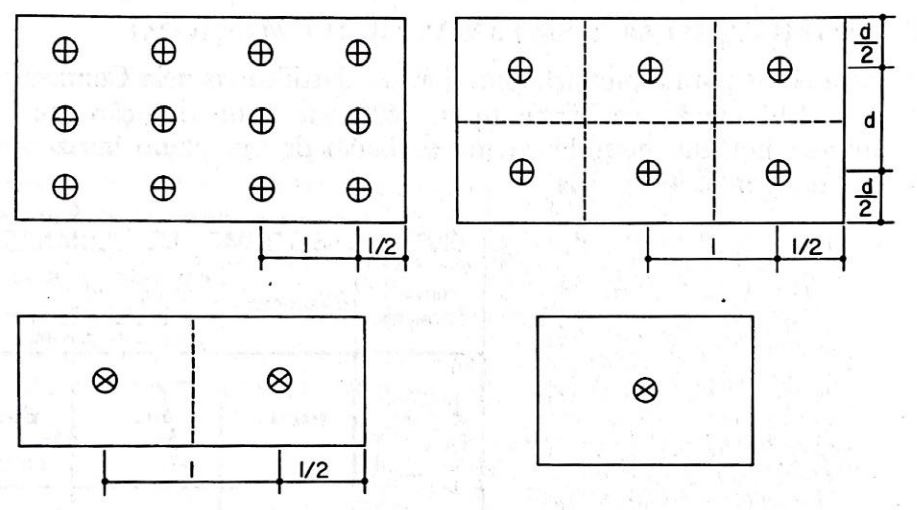
\includegraphics[width=\textwidth]{Figures/3. Lighting/light-disposicao.jpg}
			\hfill
			\caption{Disposição típicas de montagem para luminárias de iluminação de interior}  Referência \cite{de1987iluminação} p.112
			\label{fig: disposicao}
		\end{figure}
		
		\item Em instalações embutidas deverá ser utilizada a linha "PIALPLUS" da Legrand como referência técnica para interruptores e tampas
		
		\item Em instalações aparentes deverá ser utilizada a linha "Condulete TOP" da Tigre ou as linhas disponíveis da Wetzel como referência técnica para interruptores e tampas montados em conduletes de PVC
		
		\item Em instalações aparentes deverá ser utilizada as linhas disponíveis da Wetzel como referência técnica para interruptores e tampas montados em conduletes de alumínio
		
		\item\label{light:wc1}Em circuito de iluminação de banheiros e lavábulos será permitido conectar tomadas de uso geral (até 2 tomadas de 200W) ao referido circuito.
		
		\item\label{light:wc2}Em circuito de iluminação de banheiros e lavábulos será permitido conectar renovadores de ar do tipo "ventokit".
		
		\item Tomadas de uso geral não podem ser conectadas a circuitos de iluminação, a exceção das preconizadas nos itens \ref*{light:wc1} e \ref*{light:wc2}
		
		\item Em biotérios a contratada deverá prever um sistema de iluminação totalmente dimerizável
		
		\item Em Laboratórios NB3 ou NBA3 as luminárias dimensionadas serão do tipo herméricas
		\begin{enumerate}
			\item Laboratórios NB3 ou NBA3 com pavimento técnico a contratada deverá prever a remoção ou substituição dos equipamentos pelo referido pavimento, indicando em detalhe de projeto e notas
			\item Laboratórios NB3 ou NBA3 sem pavimento técnico e com forro de gesso, a contratada deverá prever em projeto que a face que possui o difusor da luminária irá facear o gesso e garantir a estanqueidade da área por sobre o gesso quando for necessário efetuar a manutenção da mesma.
			\item Demais casos deverão ser analisados pela contratada e discutidos com a Engenharia da COGIC.
		\end{enumerate}

		\item\label{light:encaixe10A}Nos caso dos encaixes rápidos utilizarem o conjunto tomada/plugue, deverá ser utilizada uma tomada de 10A
		
		\item As luminárias deverão ser projetadas tendo-se em mente a utilização de engate-rápido através de plugues e tomadas, ou dispositivos equivalentes, devendo a mesma ser indicada em nota e detalhada em projeto. Dois exemplos a seguir.
		
		\begin{figure}[H]
			\centering
			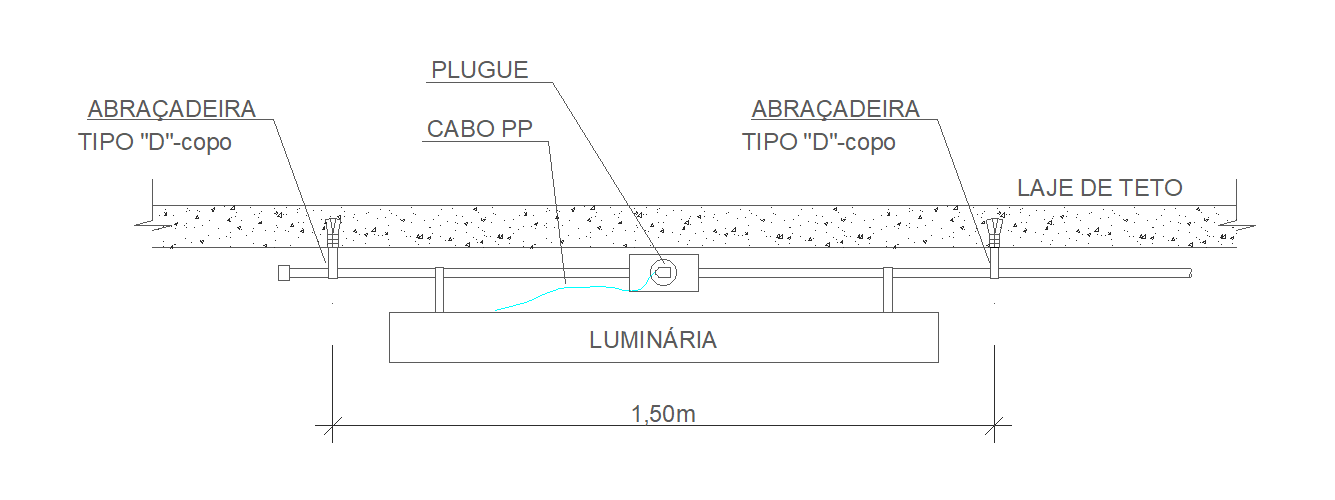
\includegraphics[width=\textwidth]{Figures/3. Lighting/light-engate rapido1.png}
			\hfill
			\caption{Encaixe rápido usando condulete e plugue de tomada ex.1}
			\label{fig: engate-rapido1}
		\end{figure}
		\begin{figure}[H]
			\centering
			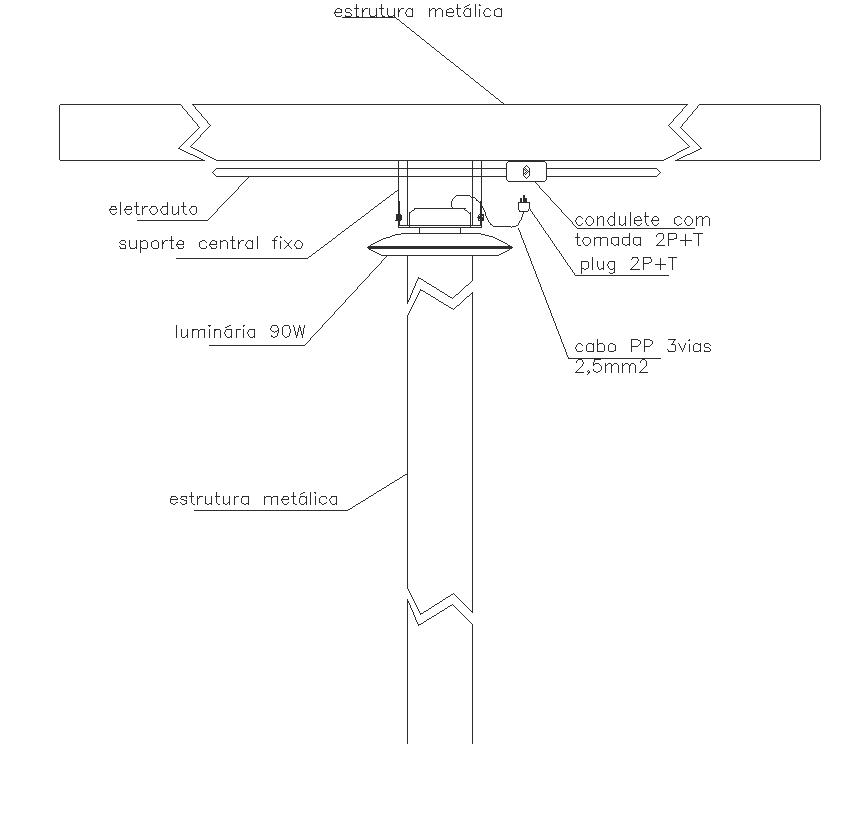
\includegraphics[scale=0.25]{Figures/3. Lighting/light-engate rapido2.png}
			\hfill
			\caption{Encaixe rápido usando condulete e plugue de tomada ex. 2}
			\label{fig: engate-rapido2}
		\end{figure}


		\item Luminárias instaladas em corredores deverão ser instaladas no sentido longitudinal a fim de obter um melhor rendimento no brilho e evitar ofuscamento. Melhores referências e explicações pode ser obtidas em \cite{simons2008lighting} p.74-75 e \cite{van2019interior} p.413.
		
		\item Luminárias em corredores só poderão ser instaladas no sentido transversal caso alguma exceção impossibilite a montagem no sentido longitudinal
	
	\end{enumerate}

% Copy this to add more chapters
\subsubsection{Iluminação de emergência e sinalização de obstáculos}


	\paragraph*{Locais de instalação}
	
	Os locais específicos onde se fazem necessária a instalação de sinalização de emergência são:
	
	\begin{figure}[H]
		\centering
		\begin{subfigure}[b]{0.3\textwidth}
			\centering
			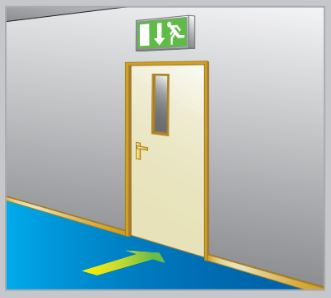
\includegraphics[width=\textwidth]{Figures/3. Lighting/light-safety1.jpg}
			\caption{A cada porta de emergência}
			\label{fig: style 1 image a}
		\end{subfigure}
		\hfill
		\begin{subfigure}[b]{0.3\textwidth}
			\centering
			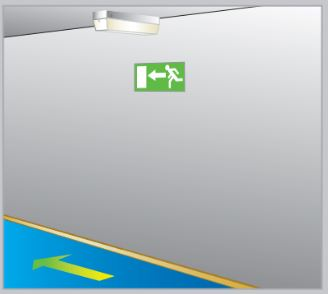
\includegraphics[width=\textwidth]{Figures/3. Lighting/light-safety2.jpg}
			\caption{Todas as sinalizações de saída}
			\label{fig: style 1 image b}
		\end{subfigure}
		\hfill
		\begin{subfigure}[b]{0.3\textwidth}
			\centering
			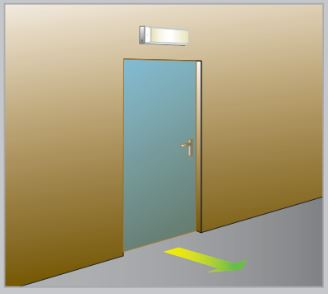
\includegraphics[width=\textwidth]{Figures/3. Lighting/light-safety3.jpg}
			\caption{Nas saídas de emergência}
			\label{fig: style 1 image c}
		\end{subfigure}
	\end{figure}

	\begin{figure}[H]
		\centering
		\begin{subfigure}[b]{0.3\textwidth}
			\centering
			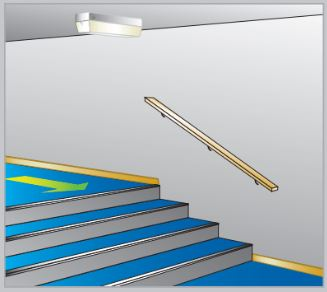
\includegraphics[width=\textwidth]{Figures/3. Lighting/light-safety4.jpg}
			\caption{Próximo escadas}
			\label{fig: style 1 image d}
		\end{subfigure}
		\hfill
		\begin{subfigure}[b]{0.3\textwidth}
			\centering
			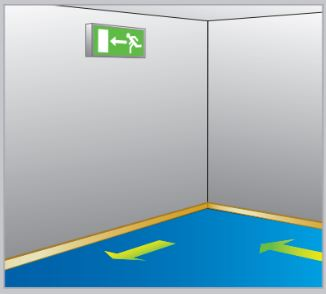
\includegraphics[width=\textwidth]{Figures/3. Lighting/light-safety5.jpg}
			\caption{Nas mudanças de direção}
			\label{fig: style 1 image e}
		\end{subfigure}
		\hfill
		\begin{subfigure}[b]{0.3\textwidth}
			\centering
			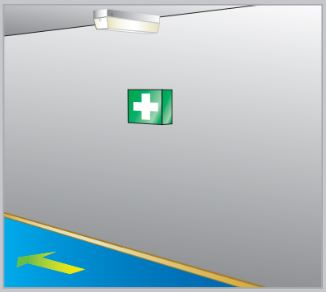
\includegraphics[width=\textwidth]{Figures/3. Lighting/light-safety6.jpg}
			\caption{Nos pontos de primeiro socorros}
			\label{fig: style 1 image f}
		\end{subfigure}
	\end{figure}

	\begin{figure}[H]
		\centering
		\begin{subfigure}[b]{0.3\textwidth}
			\centering
			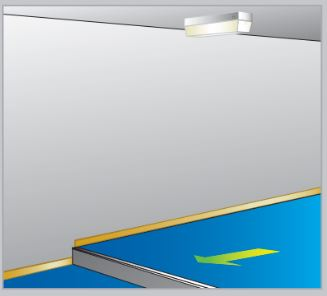
\includegraphics[width=\textwidth]{Figures/3. Lighting/light-safety7.jpg}
			\caption{A cada mudança de nível}
			\label{fig: style 1 image g}
		\end{subfigure}
		\hfill
		\begin{subfigure}[b]{0.3\textwidth}
			\centering
			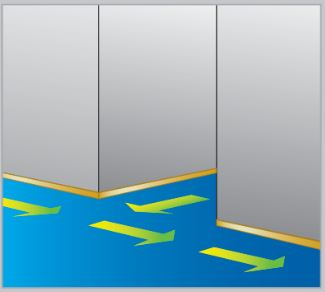
\includegraphics[width=\textwidth]{Figures/3. Lighting/light-safety8.jpg}
			\caption{Nas intersecções dos corredores}
			\label{fig: style 1 image h}
		\end{subfigure}
		\hfill
		\begin{subfigure}[b]{0.3\textwidth}
			\centering
			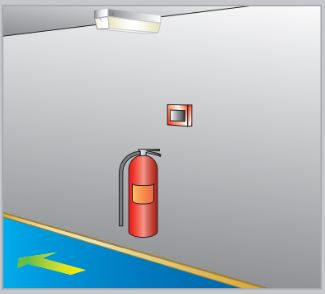
\includegraphics[width=\textwidth]{Figures/3. Lighting/light-safety9.jpg}
			\caption{Próximo a equipamentos de extinção de incêndio}
			\label{fig: style 1 image y}
		\end{subfigure}
		\caption{Localização das luminárias de emergência} fonte das imagens \cite{eaton2013} 
		\label{fig: safety-luminarires-places}
	\end{figure}

\newpage

\newpage

% Copy this to add more chapters
\subsection{Tomadas} \label{section: socket}

Sendo uma tomada um ponto de conexão que fornece energia elétrica para um plugue que será conectado, as tomadas são amplamente empregadas para ligar os mais distintos e diversos aparelhos elétricos e eletrônicos.

% Copy this to add more chapters
\subsubsection{Tomadas - Generalidades}\label{section: socket-general}

\begin{enumerate}
		
	\item Em caso de \textit{retrofit} de ambientes, pavimentos ou edificações, o número de tomadas a serem projetadas \textbf{não} podem ser dimensionadas em quantidade inferior as quantidades levantadas em campo.
	
	\item \label{socket: bitola minima} Para circuitos de tomadas, será adotado a bitola mínima de 4,0mm\textsuperscript{2}.
	
	\item \label{socket: bitola minima ar} Em circuitos de tomadas de ar-condicionado e estufas, será adotado a bitola mínima de 6,0mm\textsuperscript{2}.
	
	\item Não serão admitidas tomadas de 10A a exceção das tomadas preconizadas na seção \ref*{section: iluminacao_interiores} item \ref*{light:encaixe10A}
	
	\item Devem ser projetadas em todos os ambientes, tomadas 2P + T de 20A.
	
	\item Em postos de trabalho individualizado, devem ser previstas no mínimo 2(duas) tomadas 127V para cada posto de trabalho.
	
	\item Em laboratórios e salas de freezers deverá ser considerada a utilização de tomadas 127 e 220V.
	
	\item Em ambientes administrativos ou de ensino deverá ser considerada no mínimo a proporção de 1 tomada 220V para cada 3 ou 4 tomadas 127V (a critério do projetista e de acordo com as potências dos equipamentos)
	
	\item Não será aceita a utilização de eletrodutos de bitola menor que 1” de diâmetro para circuitos de tomadas.
	
	\item Poderá ser considerada a instalação como previsão de reserva, eletrodutos com bitolas superiores às necessárias para as bitolas iniciais dos condutores ou eletrodutos vazios.
	
	\item As tomadas de uso geral não poderão ser conectadas a circuitos de iluminação, à exceção das preconizadas nos itens \ref*{light:wc1} e \ref*{light:wc2}
	 
	\item Tomadas de uso específico deverão ser alimentadas através de circuitos individuais
	
	\item O projetista deverá dispor da forma mais uniforme possível, as tomadas nas paredes, nos rodapés ou no piso, observadas as eventuais particularidades decorrentes das condições construtivas do local e da ocupação a que se destinam.

	\item Tomadas para conectar geladeiras/freezers comuns poderão ser dispostas em até 4(tomadas) num mesmo circuito desde que as potências individuais não exceda 300W;
	
	\item Tomadas para conectar freezers com características especiais (temperaturas inferiores a 30 graus negativos) deverão ser alocados em circuitos individualizados;

	\item Para as tomadas, deverá ser adotada a bitola mínima de 4,0mm2 observando, entretanto, a diferenciação de cores nas respectivas fiações, inclusive nas redes estabilizadas e não-estabilizadas.

	\item Na especificação e cadernos de encargos ao ser confeccionado, distinguir tomadas 127V, 220V e 380V(se for o caso) e estabilizadas e não estabilizadas através do uso de cores das tampas de acabamento (quando avaliável).
	
	\item Caso existam no projeto, tomadas com tensão de 380V indicar graficamente 380V, sendo necessário constar em nota que as mesmas devem ser etiquetadas com "380V" quando executadas.
	
	\item Deve ser evitada utilização de tomadas de piso em todo o projeto, em casos excepcionais a contratante deverá ser consultada;
	
	\item Devido as características do padrão de tomadas brasileiro, indicar em projeto e na lista de materiais que as caixas conduletes / caixas de luz deverão ser adequadas para diâmetros de eletrodutos de 1”, e que as mesmas deverão ser acomodas com relativa folga;
	
	\item As tomadas deverão ser montadas em caixas conduletes(aparente) ou caixas de luz(embutidas) que permitam a instalação de eletrodutos de diâmetro mínimo de1”;
	
	\item As tomadas 127V deverão ser projetadas preferencialmente na cor branca ou bege
	
	\item As tomadas 220V deverão ser projetadas na cor vermelha;
	
		\begin{figure}[H]
			\centering
			\begin{subfigure}[b]{0.23\textwidth}
				\centering
				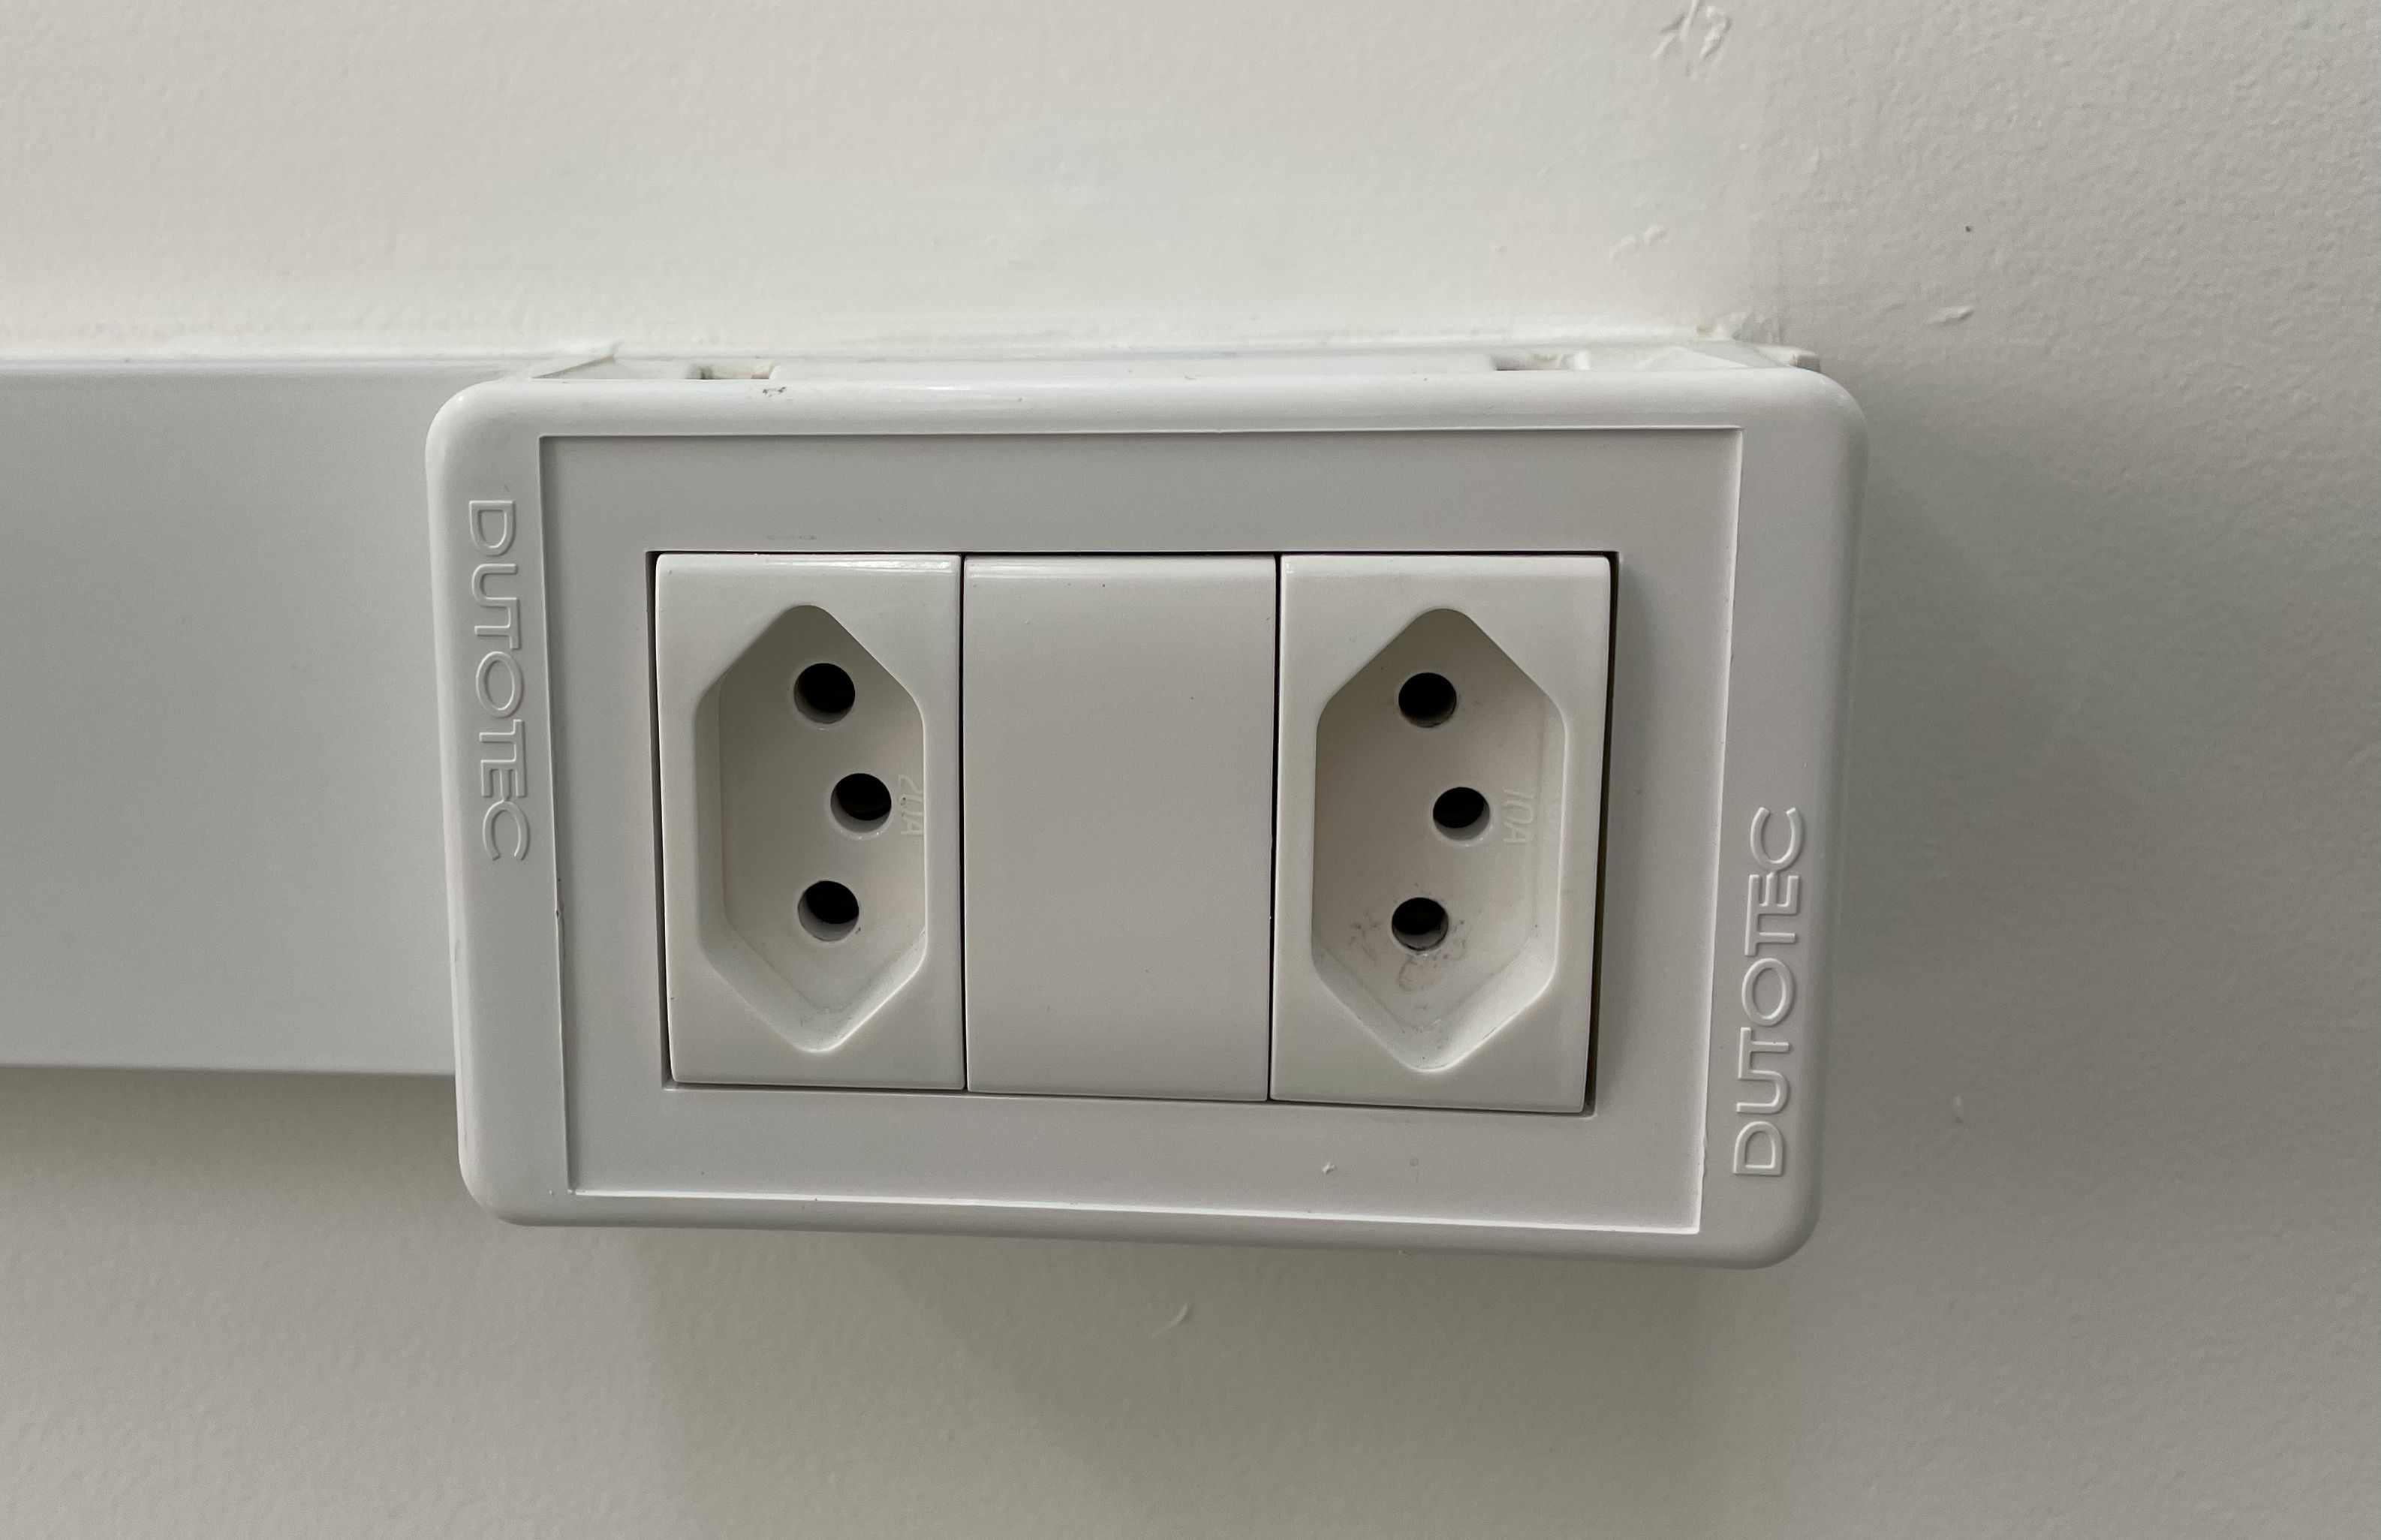
\includegraphics[width=\textwidth]{Figures/4. Socket/tomada2.jpg}
				\caption{Duas tomadas aparentes 127V (ainda não identificadas)}
				\label{fig: style 2 image a}
			\end{subfigure}
			\hfill
			\centering
			\begin{subfigure}[b]{0.23\textwidth}
				\centering
				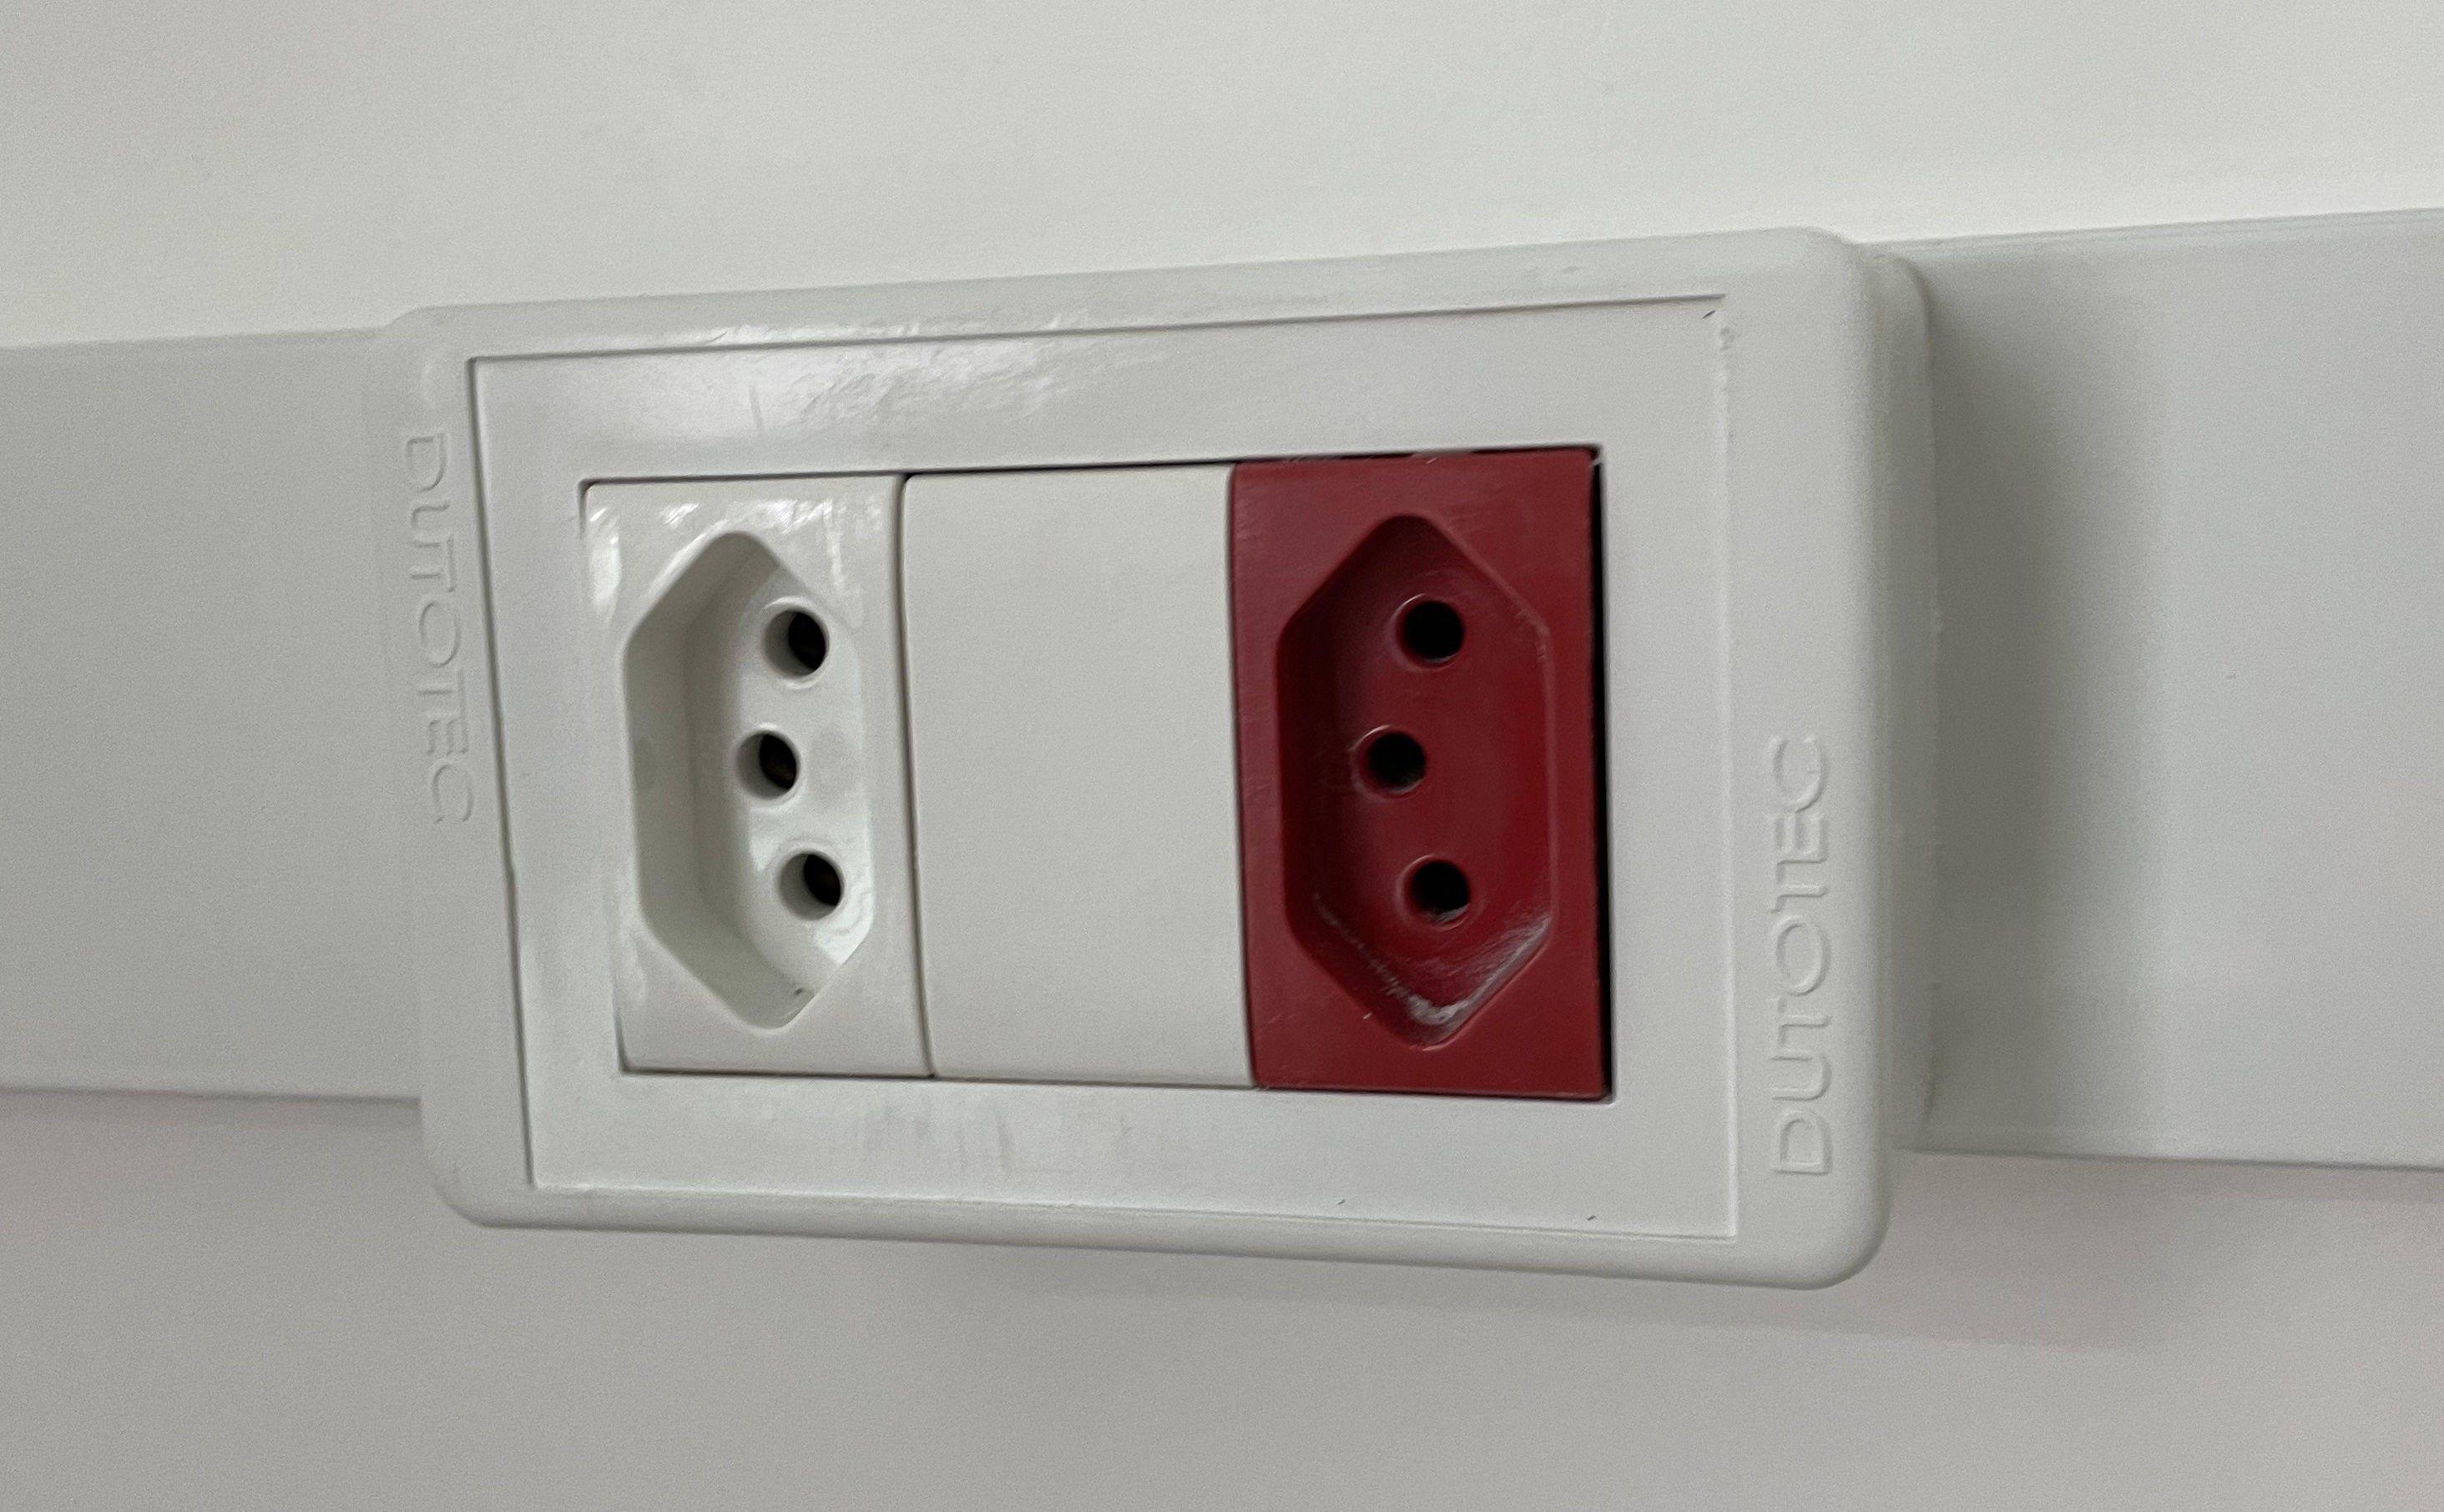
\includegraphics[width=\textwidth]{Figures/4. Socket/tomada3.jpg}
				\caption{Tomadas aparentes 127V e 220V (ainda não identificadas)}
				\label{fig: style 2 image b}
			\end{subfigure}
			\hfill
			\begin{subfigure}[b]{0.23\textwidth}
				\centering
				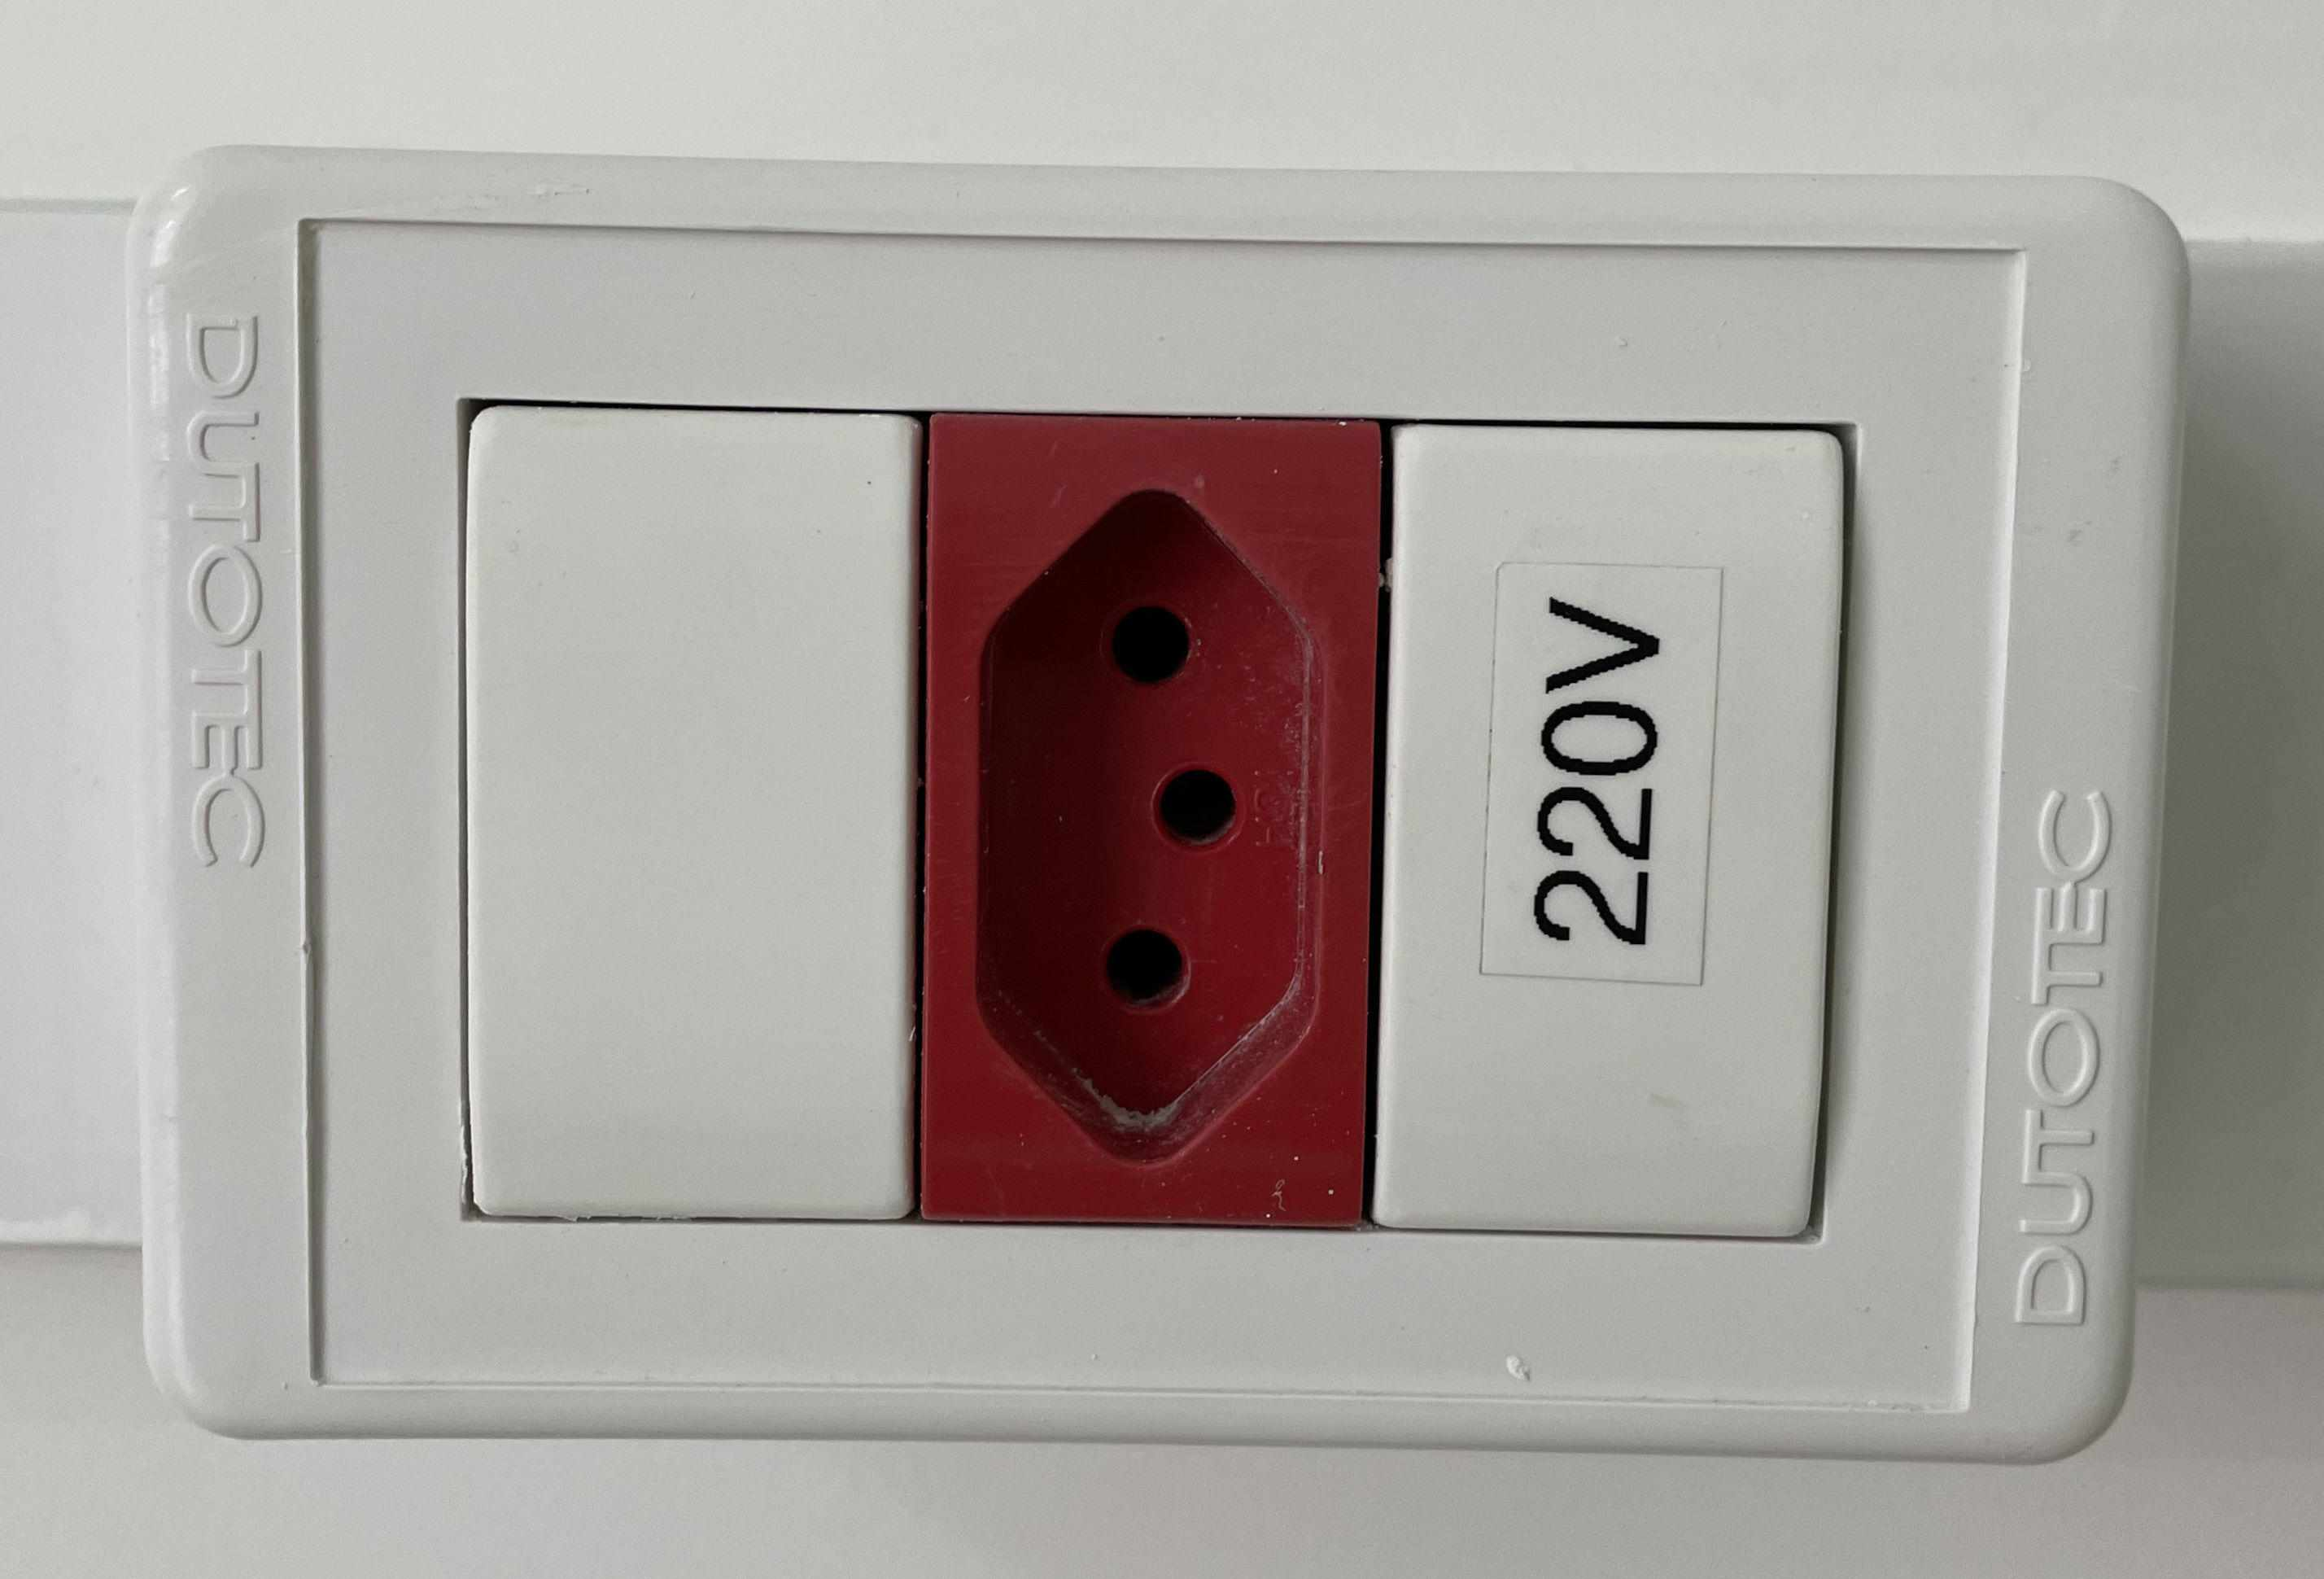
\includegraphics[width=\textwidth]{Figures/4. Socket/tomada4.jpg}
				\caption{Tomada aparente 220V já identificada}
				\label{fig: style 2 image c}
			\end{subfigure}
			\hfill
			\begin{subfigure}[b]{0.23\textwidth}
				\centering
				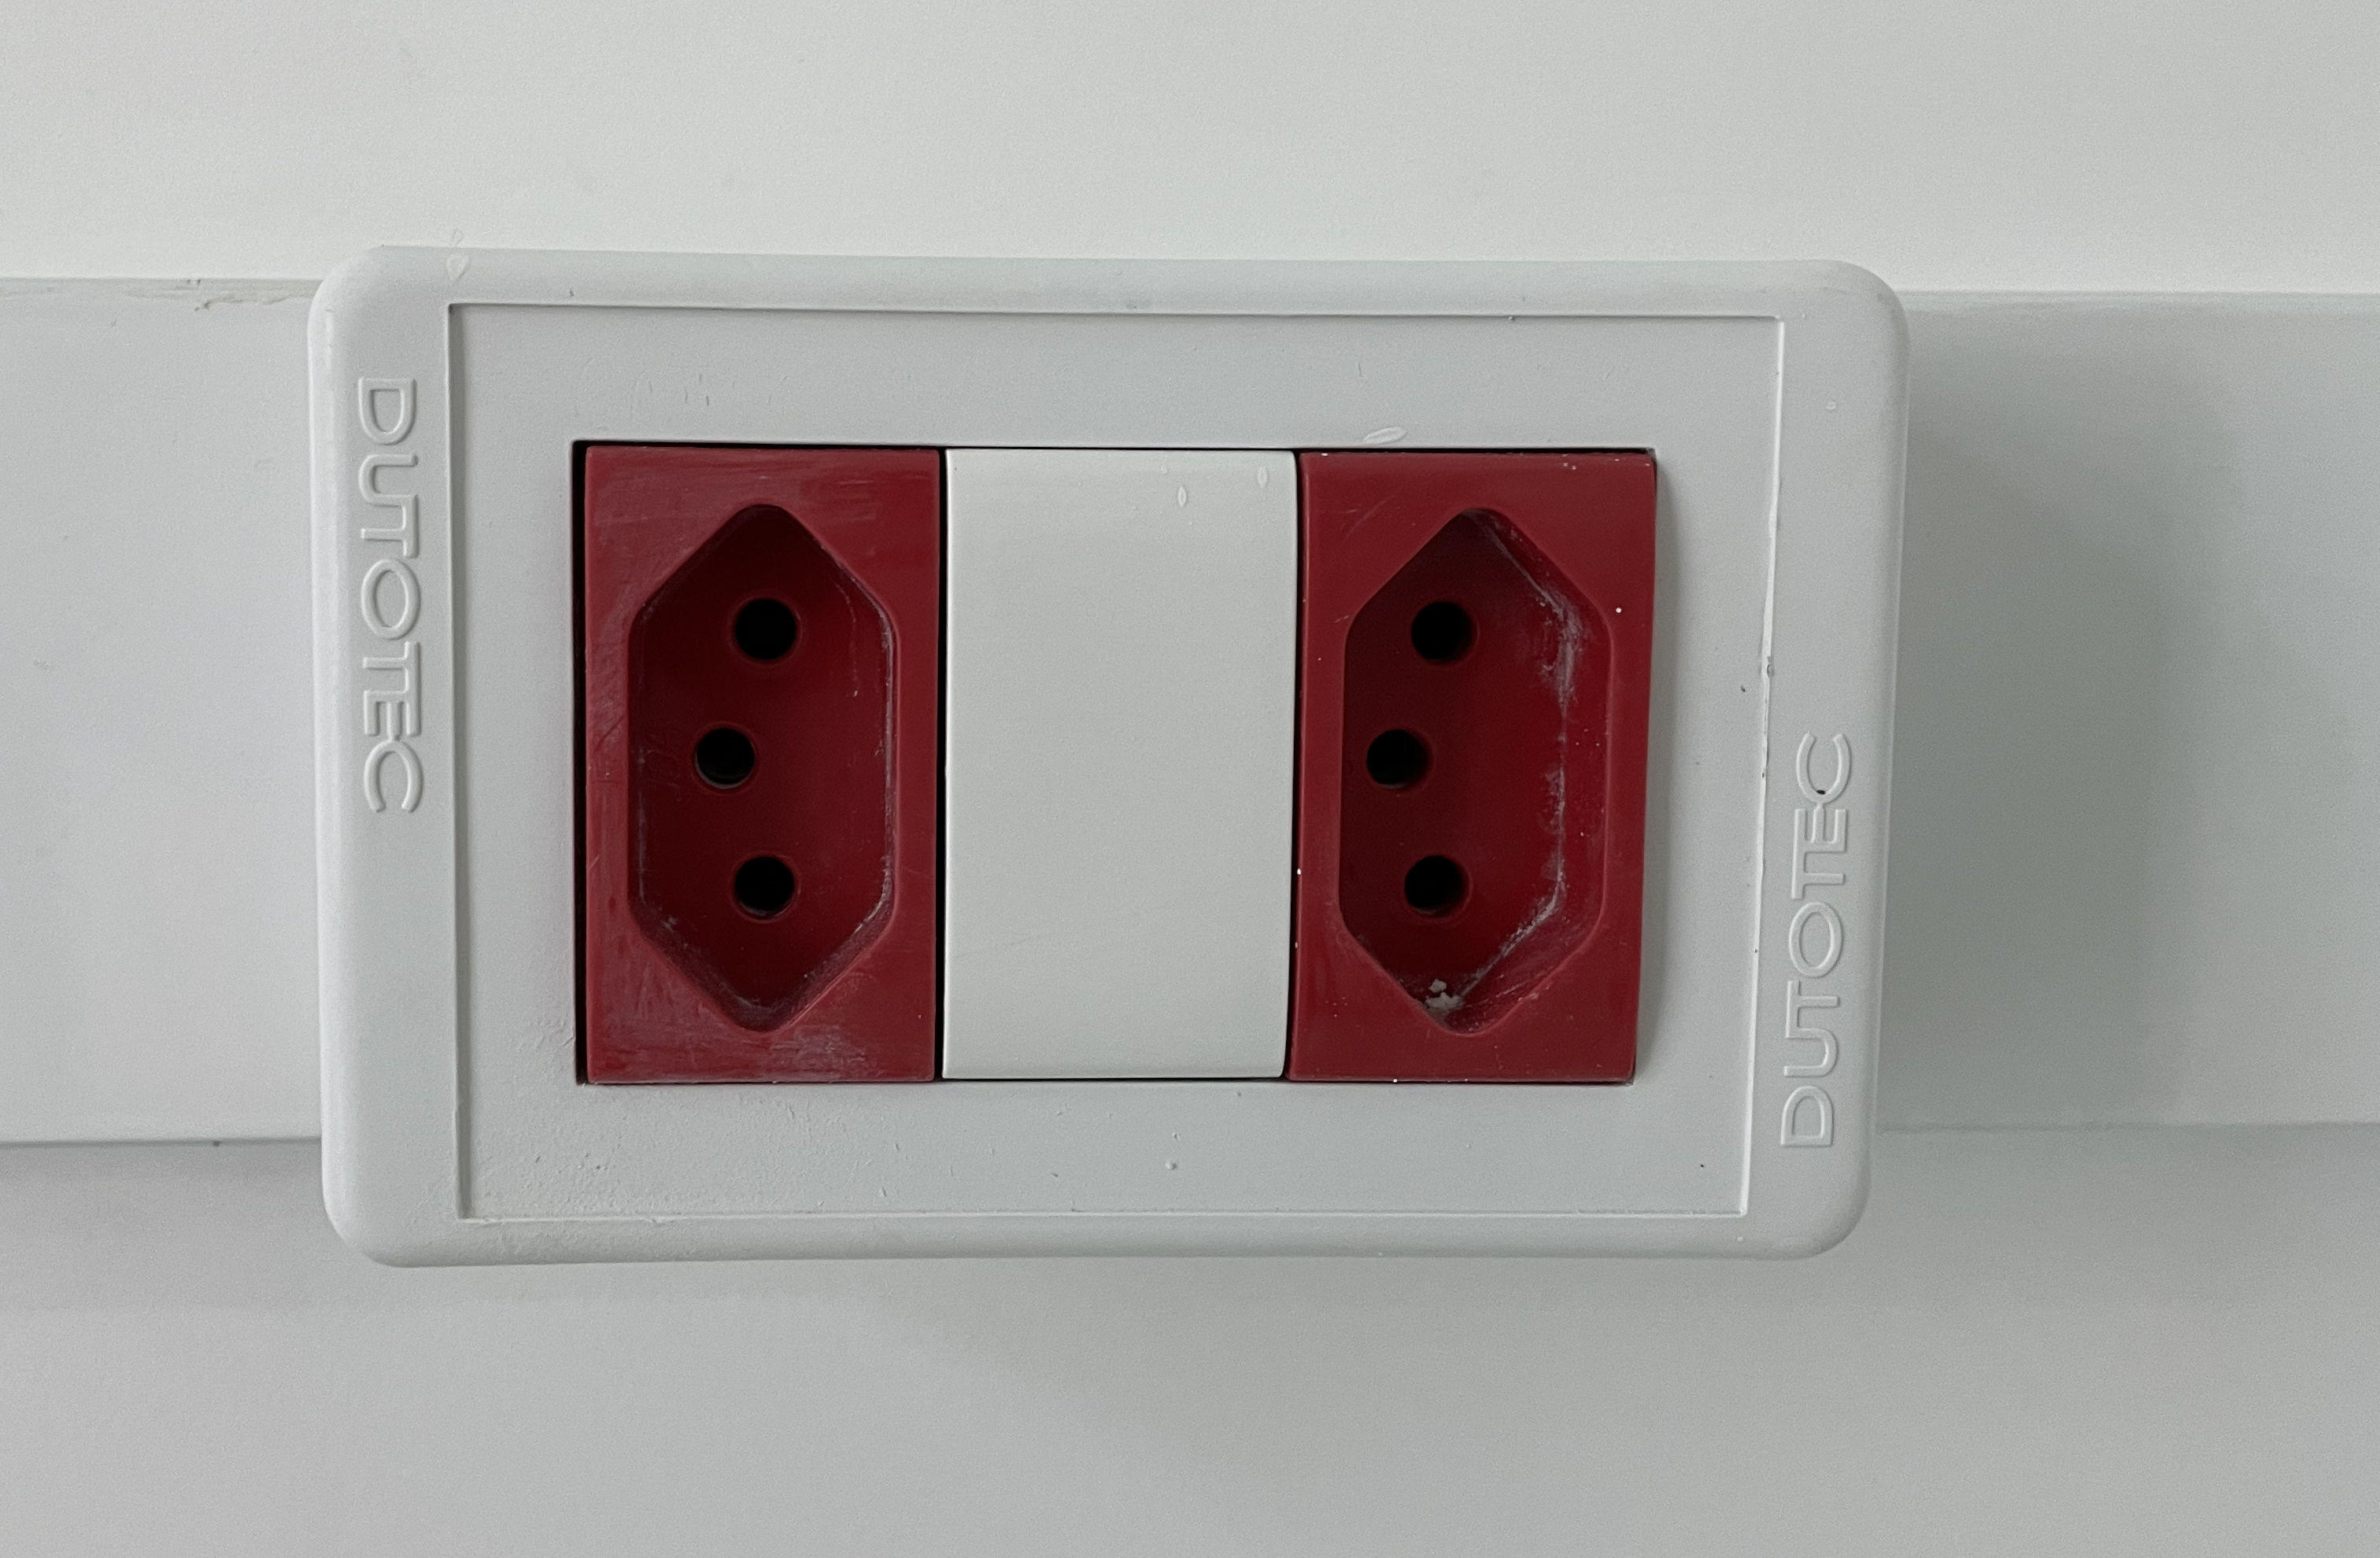
\includegraphics[width=\textwidth]{Figures/4. Socket/tomada5.jpg}
				\caption{Duas tomadas 220V (ainda não identificadas)}
				\label{fig: style 2 image d}
			\end{subfigure}
		\caption{Exemplo de tomadas em roda-meio}
		\label{fig: exemplo-rodameio}
	\end{figure}
	
	\item Existindo um projeto de sistema de segurança e alarme, a alimentação deste sistema deverá originar-se do sistema de energia ininterrupta e, o sistema deverá permanecer em funcionamento mesmo no caso de falta de energia na edificação, ou seja, deverão possuir sistemas de reserva de marcha para até 12 horas de falta total de energia.
	
	\item Ao dimensionar os eletrodutos de tomadas, os mesmos deverão ser dimensionados com diâmetro mínimo de 1"
	
	\item Potências a serem consideradas durante o desenvolvimento do projeto:
		\begin{table}[ht]
			\rowcolors{2}{Tue-red!10}{white}
			\centering
			\caption{Potências usualmente encontradas}
			\begin{tabular}[t]{ccc}
				\toprule
				\color{Tue-red}\textbf{Equipamento}&\color{Tue-red}\textbf{Pot. mínima}&\color{Tue-red}\textbf{Pot. máxima}\\
				\midrule
				Capelas&600W&600W\\
				Cabine de segurança biológica&1200W&1200W\\
				Geladeiras "comuns"&150W&300W\\
				Freezers "comuns"&150W&300W\\
				Freezers $<$ -20$^{\circ}$ C&1500W&2400W\\
				Tomadas sem carga específica(administrativo)&200W&200W\\
				Tomadas sem carga específica(laboratório)&200W&300W\\
				\bottomrule
			\end{tabular}
			\label{table: potencias}
		\end{table}

	\begin{figure}
		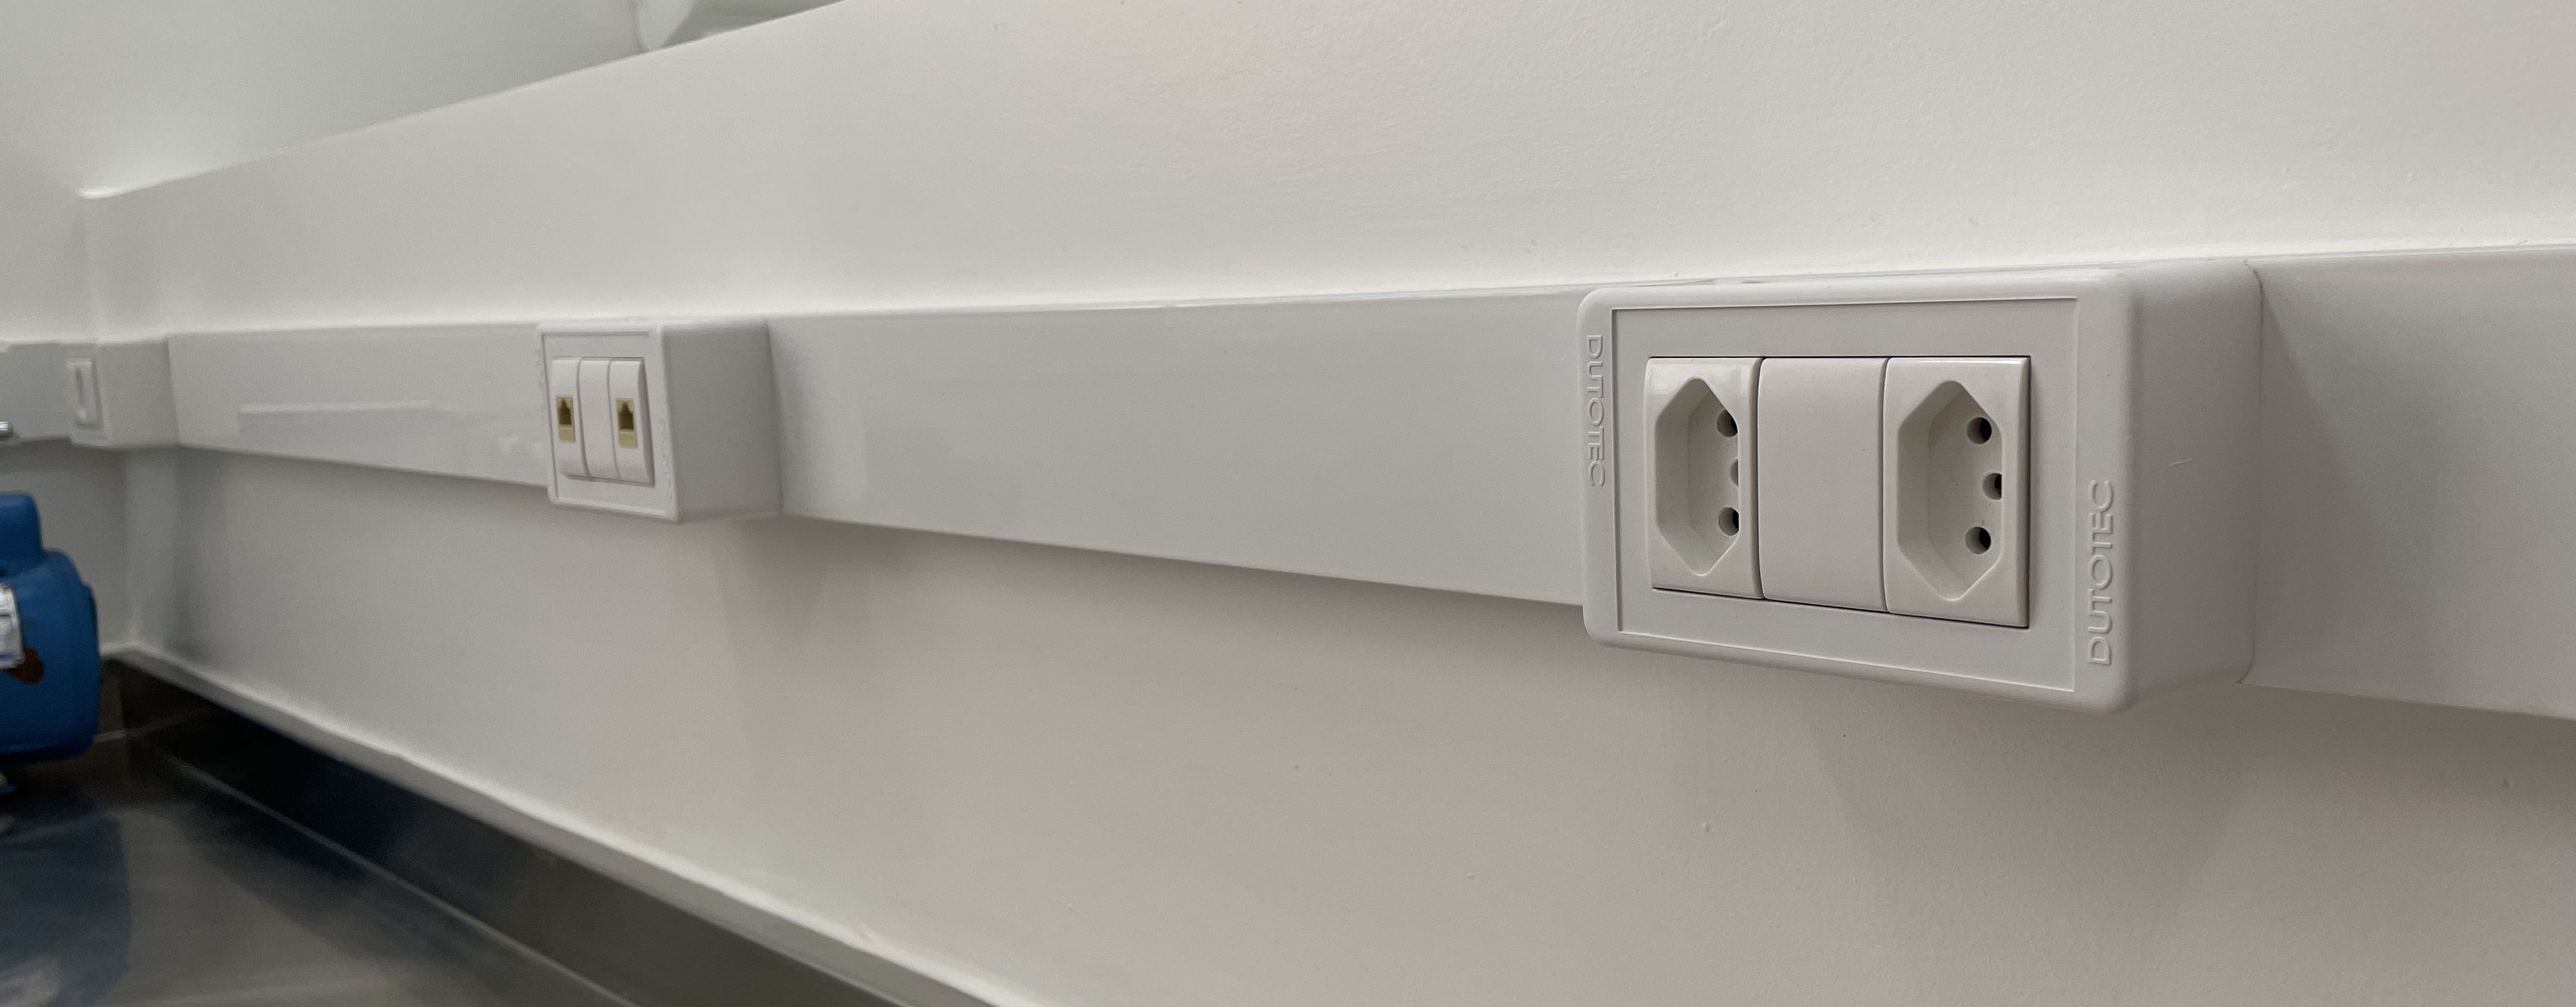
\includegraphics[width=\linewidth]{Figures/4. Socket/tomada1.jpg}
		\caption{Duas tomada 127V montada em roda-meio}
		\label{fig: tomada rodameio}
	\end{figure}
	\end{enumerate}




\newpage

% Copy this to add more chapters
\subsection{Quadros e painéis elétricos} \label{section: switchboard}
TEXTO A SER ESCRITO NESTA SECAO

% Copy this to add more chapters
\subsubsection{Generalidades}

Os itens listados nesta seção referem-se a todos os itens subsequentes de quadros apresentados a seguir.

\begin{enumerate}
	\item Deverá ser instalado em local de fácil acesso e manutenção
	\item Devem sempre que possível serem instalados nos pavimentos técnicos
\end{enumerate}

% Copy this to add more chapters
\subsubsection{Quadro geral de baixa tensão de entrada}

\begin{enumerate}
	\item O Quadro Geral de Baixa Tensão (QGBT) deverá ficar localizado na subestação quando a mesma estiver localizada dentro da edificação e o mesmo deverá prever um crescimento de até 40\% para futuras ampliações do sistema;
	\item Quando a subestação estiver localizada distante da edificação, o quadro geral de baixa tensão deverá ser instalado no interior da edificação;
	\item O QGBT deverá prever medições de tensão e de corrente individuais por fase;

\end{enumerate}

% Copy this to add more chapters
\subsubsection{Quadro de distribuição} \label{switchboard: distribuicao}

\begin{enumerate}

	\item Instalação dos quadros de distribuição em local de fácil acesso para operação e manutenção. Localizar o quadro de distribuição, sempre que possível no pavimento técnico e próximo ao centro das cargas e de tal modo que a extensão dos circuitos a ele associados não ultrapasse 40m.
	
	\item No caso da inexistência ou impossibilidade de instalação no pavimento técnico, os quadros de distribuição deverão ser instalados preferencialmente nas áreas técnicas ou próximos aos \textit{shafts}, sempre próximos ao centro das cargas.
	
	\item Devem ser projetados disjuntores de acordo com a norma IEC 947-2, como dispositivos de proteção dos circuitos.;
	
	\item Prever disjuntores de reserva (20\%), deixando espaços vazios para futuras adições de disjuntores na proporção de um para cada cinco disjuntores ativos.
	
	\item Os quadros gerais deverão sempre ser dotados de disjuntores gerais com classe de corrente e tensão projetadas a critério do projetista;
	
	\item Prever protetores de surtos em todos os quadros de distribuição gerais parciais (não se aplica aos quadros de distribuição terminais);

\end{enumerate}

% Copy this to add more chapters
\subsubsection{Quadro de iluminação e tomadas}\label{switchboard: iluminacao}

\begin{enumerate}
	
	\item Em áreas com grande número de salas e circuitos, o projetista deverá propor uma individualização de quadros elétricos parciais por sala ou grupo de salas, de maneira a minimizar a quantidade de circuitos instalados nos quadros de distribuição gerais;
	
	\item No caso de áreas laboratoriais, um quadro de baixa tensão deverá ser instalado junto à entrada de cada laboratório, em local de fácil acesso e manutenção e, o mesmo servirá para alimentação dos pontos de iluminação e tomadas propostos pelo projetista, desta forma os circuitos serão individualizados por laboratório.
	
	\item Poderá ser proposto, a critério do projetista de acordo com a carga instalada em cada laboratório, a utilização de 1(um) quadro elétrico para cada 2(dois) laboratórios;
	
	\item Nos demais casos o projetista deverá avaliar a melhor solução técnica a ser aplicada.
	
\end{enumerate}

% Copy this to add more chapters
\subsubsection{Quadro de ar-condicionado}

\begin{enumerate}
	\item Deverá ser instalado em local de fácil acesso e manutenção e, o mesmo servirá para alimentação dos pontos de condicionadores de ar a serem instalados.
	
	\item As premissas previstas para quadro de distribuição vistas na seção \ref{switchboard: distribuicao} e quadro de baixa tensão de iluminação e de tomadas vistas na seção \ref{switchboard: iluminacao} são válidas para os quadros de baixa tensão de ar-condicionado.

\end{enumerate}

% Copy this to add more chapters
\subsubsection{Quadro de baixa tensão do(s) NOBREAK(s)}

\begin{enumerate}
	\item Deverá ser instalado em local de fácil acesso e manutenção e sempre que possível instalado no pavimento técnico e, o mesmo servirá para alimentação dos pontos de energia estabilizada a serem instaladas.
	\item Sempre deverá ser previsto um sistema de by-pass, de modo que em caso de manutenção ou problemas operacionais o ramal de alimentação das cargas estará sempre em linha;
	\item As premissas previstas para quadrods de distribuição vistas na seção \ref{switchboard: distribuicao} e quadro de baixa tensão de iluminação e de tomadas vistas na seção \ref{switchboard: iluminacao} são válidas para os quadros de baixa tensão de nobreaks.
\end{enumerate}

\newpage

\newpage

% Copy this to add more chapters
\subsection{Nobreaks} \label{section: nobreak}
TEXTO A SER ESCRITO

\subsubsection{Generalidades}
\begin{enumerate}
	\item Quando o projeto de distribuição elétrica exigir, deverá ser previsto a utilização de sistema de nobreak’s que sejam compatíveis e, possibilitem serem alimentados a partir dos grupos motor geradores de emergência (GMGs) a serem instalados no sistema. 
	
	\item Os nobreak’s deverão possuir conjuntos de baterias que possibilitem uma autonomia mínima de 15 minutos para todo o sistema de energia estabilizada.
	
	\item Os nobreak’s projetados deverão possuir obrigatoriamente entrada trifásica e saída trifásica. Casos excepcionais, a contratada deverá ser consultada.
	
	\item Sempre deverá ser previsto um sistema de by-pass, de modo que em caso de manutenção ou problemas operacionais o ramal de alimentação das cargas estará sempre em linha;
	
	\item Condições específicas serão vistas posteriormente.
	
	\item Nos casos que se faça necessário o uso de redundância de \textit{nobreaks} e o contratante não estabeleça o tipo de redundância(\textit{BACKUP}) a ser empregado, caberá ao projetista propor o tipo de redundância a ser empregado (de acordo com o item \ref{nobreak: tipo de redundancia}) e obter aprovação do contratante.
	
	\item Possíveis redundâncias de nobreak's caso seja necessária.
	\begin{enumerate}\label{nobreak: tipo de redundancia}
		\item Redundância em cascata/\textit{by-pass}, figura \ref{fig: redundancia1}
		
		\item Paralelismo redundante, figura  \ref{fig: redundancia2}
		
		\item Paralelismo N + 1, figura  \ref{fig: redundancia3}
		
		\item Paralelismo modular, figura  \ref{fig: redundancia4}
		
		\item Outras indicadas pela contratada
		
	\end{enumerate}

	\begin{figure}[H]
		\centering
		\begin{minipage}{0.45\textwidth}
			\centering
			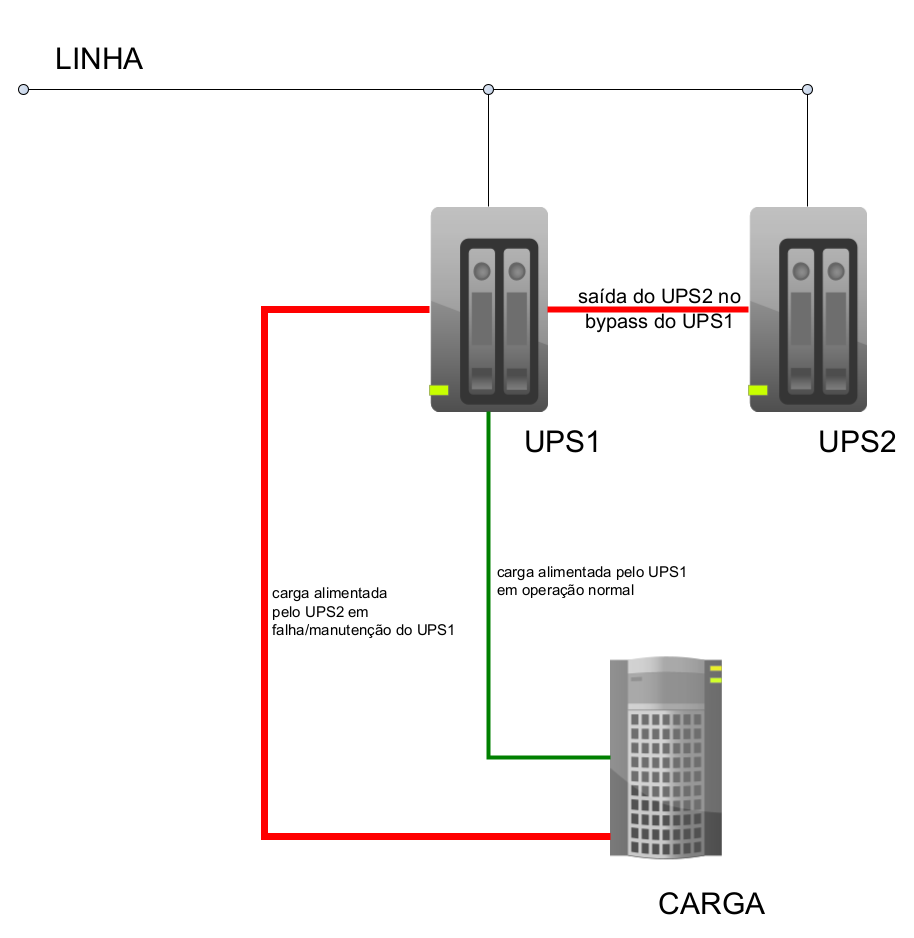
\includegraphics[width=\textwidth]{Figures/7. nobreak/redundancia1.png}
			\captionof{figure}{Redundância em cascata/by-pass}
			\label{fig: redundancia1}
		\end{minipage}
		\hfill
		\begin{minipage}{0.45\textwidth}
			\centering
			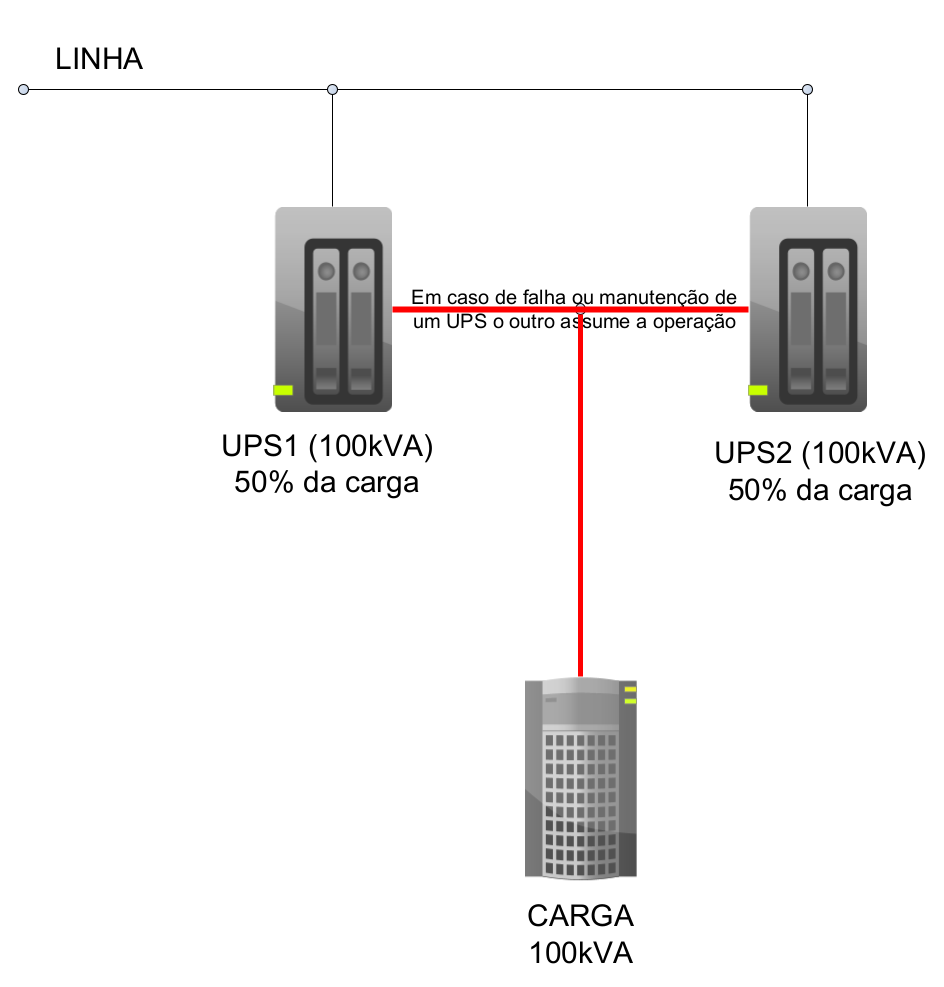
\includegraphics[width=\textwidth]{Figures/7. nobreak/redundancia2.png}
			\captionof{figure}{Paralelismo redundante}
			\label{fig: redundancia2}
		\end{minipage}
	\end{figure}
	\begin{figure}[H]
	\centering
		\begin{minipage}{0.45\textwidth}
			\centering
			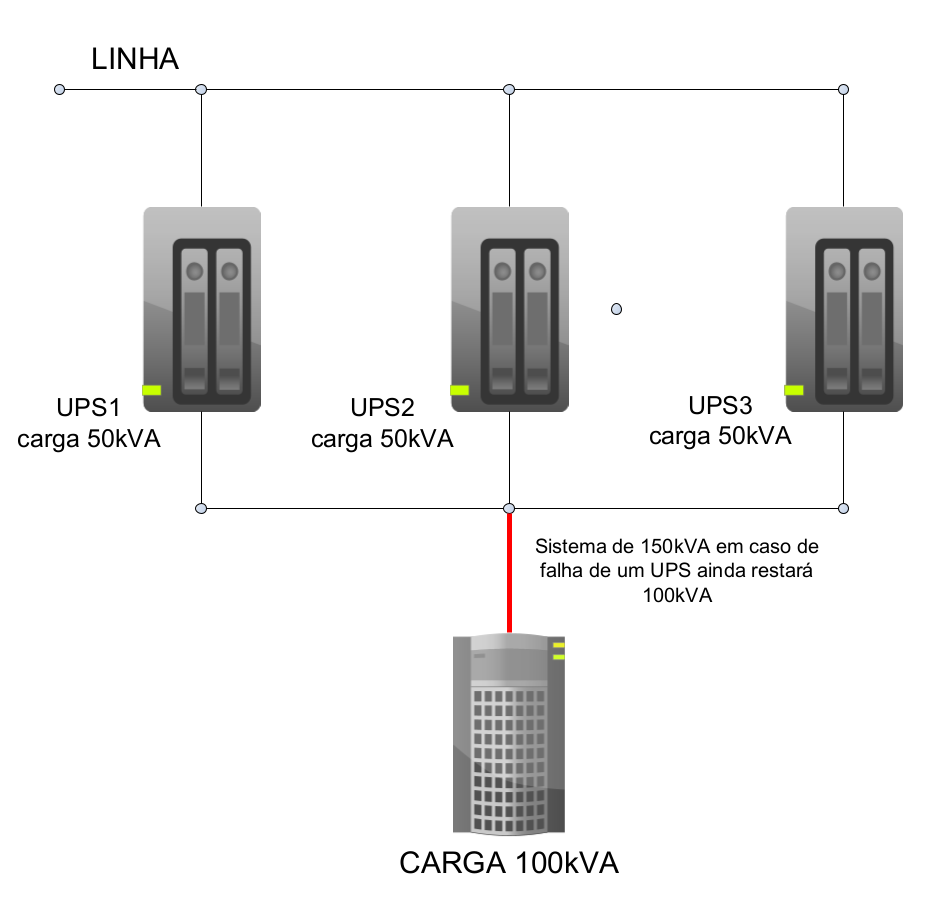
\includegraphics[width=\textwidth]{Figures/7. nobreak/redundancia3.png}
			\captionof{figure}{Paralelismo N + 1}
			\label{fig: redundancia3}
		\end{minipage}
		\begin{minipage}{0.45\textwidth}
			\centering
			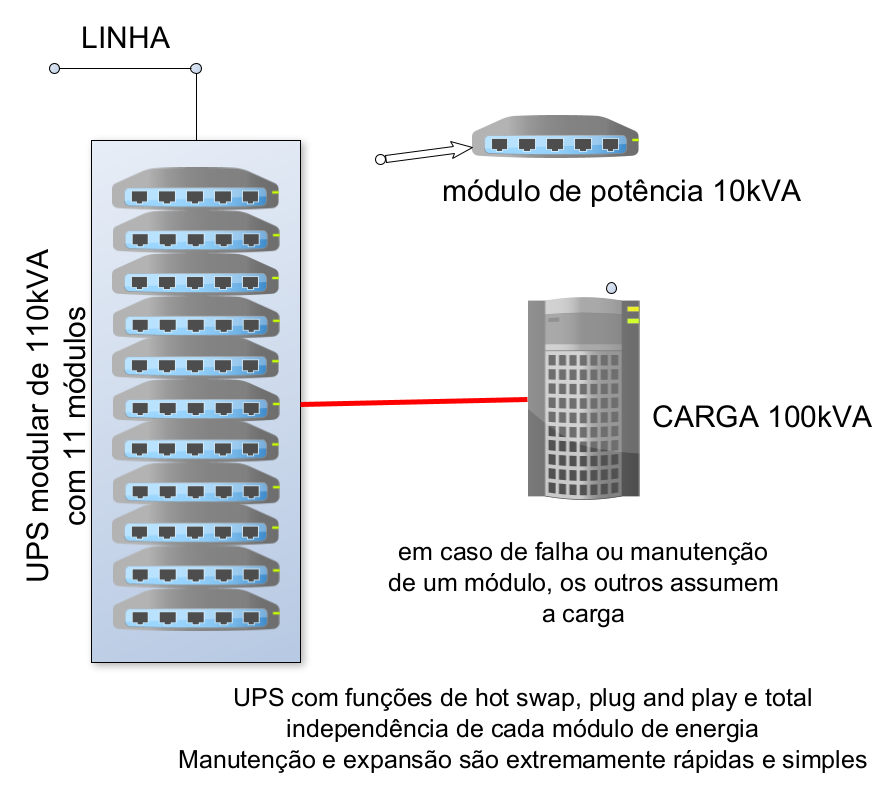
\includegraphics[width=\textwidth]{Figures/7. nobreak/redundancia4.png}
			\captionof{figure}{Paralelismo modular}
			\label{fig: redundancia4}
		\end{minipage}
	\end{figure}

\end{enumerate}
\newpage

% Copy this to add more chapters
\subsection{Encaminhamento e ramal de alimentação} \label{section: encaminhamento}
TEXTO A SER ESCRITO EM VERSAO FUTURA

% Copy this to add more chapters
\subsubsection{Generalidades}

\begin{enumerate}
	\item O projeto de distribuição elétrica das áreas que passarão pelas intervenções necessárias à implantação das instalações do projeto deverá prever, dentro do possível, uma flexibilidade que possibilite futuras ampliações com o mínimo de obras e paralisações. 
	
	\item Sempre que possível projetar preferencialmente leitos de cabos ou eletrocalhas, instaladas no pavimento técnico;
	
	\item Quando o projeto não houver previsão de pavimento técnico, o caminhamento preferencialmente dar-se-á através de leitos ou eletrocalhas por sobre áreas de circulação comum devendo o projetista evitar ao máximo passar o encaminhamento principal por sobre salas, laboratórios e dentre outras áreas que não são de uso coletivo;
	
	\item Os encaminhamentos secundários podem ser dimensionados através de eletrodutos ou eletrocalhas; 
	
	\begin{figure}[H]
		\centering
		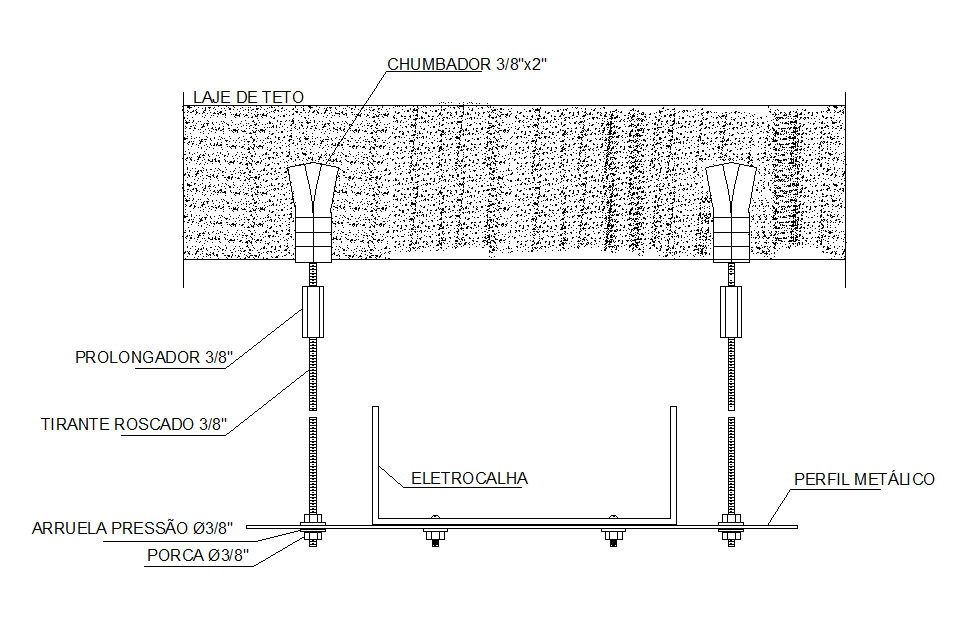
\includegraphics[scale=.30]{Figures/5. Hardware/eletrocalha-fixacao1.png}
		\caption{Eletrocalha fixada através de tirantes}
		\label{fig: eletrocalha fixacao1}
	\end{figure}
	
\end{enumerate}

% Copy this to add more chapters
\subsubsection{Ramal de alimentação dos pavimentos}

\begin{enumerate}
	\item Cada pavimento deverá contar com uma alimentação individual normal, emergência e ininterrupta (estas duas últimas quando aplicáveis a depender do projeto a ser desenvolvido), sendo previsto um crescimento de 40\% da carga ao longo de 5 anos. Deverá ser considerada a necessidade de um detalhamento no projeto do encaminhamento e interligação do Quadro de Geral de Baixa Tensão ao ponto de entrega do andar;
	
	\item A circulação destes circuitos de alimentação sempre que possível devem ser projetados preferencialmente em leitos de cabos e/ou eletrocalhas nos pavimentos técnicos (se estes existirem no projeto)
	
	\item Em caso de inexistência de pavimento técnicos, o caminhamento de leitos ou eletrocalhas deverá seguir preferencialmente em áreas de circulação comuns;
	
	\item A utilização de salas ou laboratórios para passagens de eletrocalhas/leitos de que conterão ramais de alimentação gerais ou de ramais de alimentação parciais estará proibida e casos excepcionais, a contratante deverá obrigatoriamente ser consultada;
	
	\item Deverá ser considerada a necessidade de um detalhamento no projeto do encaminhamento e interligação do quadro de geral de baixa tensão ao ponto de entrega do andar;

\end{enumerate}

% Copy this to add more chapters
\subsubsection{Linhas de distribuição (condutores)}

\begin{enumerate}
	\item A bitola mínima dos circuitos terminais deverá ser de acordo as estabelecidas na seção \ref{lighting - generalidades} item \ref{lighting: bitola minima} e seção \ref{section: socket-general} itens \ref{socket: bitola minima} e \ref{socket: bitola minima ar} ;
	\item Dimensionar a bitola do condutor conforme a capacidade de condução de corrente e a queda de tensão admissível, considerando os fatores de correção de temperatura de agrupamento de cabos. 
	\item Limitar a queda de tensão, entre a origem da instalação e qualquer ponto de utilização, a valores compatíveis com a norma NBR 5410. 
	\item Dimensionar os alimentadores de modo a transmitir potência suficiente aos circuitos alimentadores, bem como para atender a futuros aumentos de carga. 
	\item Dimensionar, especificar e identificar os circuitos de acordo com a NBR-5410.

	
\end{enumerate}

\newpage

% Copy this to add more chapters
\section{Referências técnicas - média tensão} \label{section: tech references medium}
TEXTO A SER ESCRITO NESTA SECAO

TODOS OS TEXTOS DESTA SECAO PRECISAM SER COMPLEMENTADOS

% Copy this to add more chapters
\subsection{Subestação} \label{section: power plant}

Para controlar e transformar um fornecimento de energia em média tensão para baixa tensão, é necessário um ou mais subestações. Elas devem ser projetadas para atender aos requisitos que se aplicam a localidade as quais elas serão implantadas.

As regulamentações abrangem questões como proteção contra choques, tensão de passo, incêndio, segurança, rotas de fuga, dentre outros. Para garantir o cumprimento destes requisitos é aconselhável empregar um consultor experiente (engenheiro pleno ou sênior).

\subsubsection{Generalidades}

\begin{enumerate}
	\item A subestação principal de entrada deverá ser projetada segundo as características padronizadas da concessionária local de energia elétrica; (se aplicável)
	
	\item O dimensionamento e a inserção no sistema de suprimento de energia elétrica do prédio dos grupos moto-geradores de emergência com capacidade necessário e suficiente a alimentação de todas as cargas a eles previstas (iluminação, tomadas e ar-condicionado); (se aplicável)
	
	\item Os grupos moto-geradores deverão ser providos de Regulador Eletrônico de Tensão (REV), assim como, possuir características construtivas que possibilitem a alimentação de cargas não deformantes, equipamentos de informática. (se aplicável)
	
	\item Os Grupos Motor Geradores deverão ser providos de Sistema de Transferência Ininterrupta de Carga em Rampa (STR) para Grupos Geradores com operação em paralelo com a rede (se aplicável);	
	
\end{enumerate}


% Copy this to add more chapters
\subsection{Ramal de entrada de energia elétrica e medição} \label{section: entrance}

\begin{enumerate}
	\item O dimensionamento do ramal de entrada e da medição de energia elétrica deverá seguir os padrões propostos pela concessionária local de energia elétrica a época do desenvolvimento do projeto;

	\item Deverá ser descrito, dimensionado e detalhado conforme as normativas técnicas da concessionária local de energia elétrica;
		
	
\end{enumerate}


\newpage

% Copy this to add more chapters
\section{Etapas básicas para elaboração de projeto de elétrica} \label{section: referencias}

(PRECISA SER ESCRITA UMA INTRODUCAO)
\begin{enumerate}
	\item Levantamentos
	\item Estudo preliminar 
	\item Anteprojeto
	\item Projeto Executivo 
\end{enumerate}

% Copy this to add more chapters
\subsection{Levantamento} \label{subsection: etapa-LV}
[ TEXTO A SER ESCRITO EM VERSÃO FUTURA]

\subsubsection{Generalidades}
	\begin{enumerate}

		\item XXXXXXXXXXXXXXXXXXXXXXXXXX
			\begin{enumerate}
				
				\item XXXXXXXXXXXXXXXXXXXXXXXXXXXXXXXXXXXXXXXXXXXXXXXXXXXXXXXXXX
			
			\end{enumerate}
		
		\item XXXXXXXXXXXXXXXXXXXXXXXXXXXXXXXXXXXXXXX
	\end{enumerate}



% Copy this to add more chapters
\subsection{Estudo preliminar} \label{subsection: estudo preliminar}

TEXTO A SER ESCRITO EM VERSÃO FUTURA

\subsubsection{Generalidades}

\paragraph{Visita técnica ao local de implantação dos projetos}

	\begin{enumerate}
	
		\item Apresentar documento de visita técnica validado por funcionários do setor de manutenção da Fiocruz.
		\item Deverá ser preparado e entregue um documento indicando as áreas visitadas, dias, pessoas contatadas e atas de reuniões com as informações obtidas nessa visita.
		\item Um profissional da CONTRATANTE deverá acompanhar a visita técnica, devendo ser agendada a data e horário de visita. Esse documento deverá ser assinado pelo responsável técnico pelo projeto e pelos funcionários da Fiocruz, lotados nos setores anteriormente citados, que acompanharam a visita do profissional responsável.
	\end{enumerate}

\paragraph{Levantamento das informações básicas sobre o local de implantação do projeto}
	\begin{enumerate}
		\item Relatório com fotos e pareceres técnicos sobre as instalações e ambientes físicos existentes no local, incluindo análises relativizando as informações recolhidas nesta Etapa, com o estudo conceitual fornecido pela Fiocruz e com os requisitos técnicos e legais exigidos.
		
		\item Levantar as redes externas de elétrica existentes no local e analisar o impacto causado a elas pela implantação do projeto. 
		
		\item Programa básico das instalações de elétrica com justificativa e descrição dos sistemas propostos.
		
		\item Elaboração do estudo comparativo técnico e econômico das alternativas técnicas para os sistemas, aliando preço, facilidade e tempo de execução.
		
		\item Complementação da planilha de máquinas e equipamentos para a edificação com a descrição das informações e características dos aparelhos indicando os dados informados pelo usuário. 
		
		\item Apresentação em arquivo eletrônico (.doc e .pdf) e 01 impressão em formato A4 encadernada e assinada pelo responsável técnico.
	\end{enumerate}

\paragraph{Relatório preliminar}
		\begin{enumerate}
			\item Estudo preliminar desenvolvido segundo as normas(??????).
			
			\item Vistoria do entorno e do terreno onde será erguida a edificação.

			\item Levantamento dos serviços públicos existentes.
			
			\item Consulta à legislação pertinente e órgãos públicos envolvidos na aprovação do projeto.
			
			\item Deverão ser apresentados nesta etapa, sob forma de memorial descritivo, os seguintes documentos:
			
			\item Plantas de situação, indicando o terreno e seu entorno imediato onde ocorrerão as intervenções junto à concessionária local.
			
			\item Plantas baixas de localização das edificações, subestação (se aplicável) e demais edículas.
			
			\item Definição dos índices de iluminação a serem adotados.
			
			\item Levantamento de quantidades e potências dos pontos de consumo.
			
			\item Levantamento das cargas.
			
			\item Localização e pré-dimensionamento dos equipamentos sugeridos pelo autor do projeto (transformadores, geradores, bombas, etc.).
			
			\item Definição do sistema de alarme, pontos a serem protegidos e tipos de sensores.
			
			\item Apresentação em arquivo eletrônico (.dwg e .pdf) e 01 impressão em formato apropriado assinada pelos profissionais responsáveis.
		\end{enumerate}

\subsubsection{Produtos a serem entregues}

\begin{enumerate}
	\item Relatório de vistoria do local de implantação atestado por um funcionário da FIOCRUZ.
	\item Relatório das análises das visitas aos órgãos públicos e concessionárias(se aplicável)
	\item Relatório com fotos e pareceres técnicos sobre as instalações e ambientes físicos existentes no local, incluindo análises relativizando as informações recolhidas nesta Etapa, com o estudo preliminar fornecido pela FIOCRUZ e com os requisitos técnicos e legais exigidos. 
	\item Descritivo básico com indicação das alternativas e recomendações de ordem técnica para adequação ao projeto de arquitetura e documentos gráficos para elucidar as proposições técnicas, incluindo, entre outros de ordem legal: Dados da consulta prévia a concessionárias de energia elétrica; (se aplicável)
	\item Programa de necessidades arquitetônicas por ambiente (necessária consulta aos projetos de arquitetura, ar-condicionado, telecomunicações e CFTV).
	\item Programa básico das instalações elétricas incluindo memória de cálculo preliminar, com justificativa dos sistemas propostos além da determinação dos requisitos e materiais acústicos para atenuação do ruído provocado pelo gerador a ser instalado em ambiente específico. (se aplicável)
	\item Localização e características da rede pública de fornecimento de energia elétrica; (se aplicável)
	\item Identificação da tensão local de fornecimento de energia elétrica (primária e secundária); 
	\item Descrição básica do sistema de fornecimento de energia elétrica: entrada, transformação, medição e distribuição - da área de intervenções, distribuição em baixa tensão, iluminação e tomadas, sistema de distribuição de pontos de força, sistema de alarme de segurança, fontes de emergência e pontos de alimentação emergenciais; 
	\item Descrição das informações e características dos aparelhos elétricos vinculados às plantas de layout e com os dados informados pelo usuário; 
	\item Descrição básica do sistema de aterramento e/ou proteção contra descargas atmosféricas, caso necessário;
	\item Determinação básica dos espaços necessários para as centrais de energia;
	\item Determinação básica das áreas destinadas ao encaminhamento horizontal e vertical do sistema elétrico (prumadas);
	\item Previsão de consumo de energia elétrica;
	\item Elaboração do estudo comparativo técnico e econômico das alternativas técnicas para o sistema;
	\item Pré-localização do sistema de distribuição, prumadas dos leitos/eletrocalhas/eletrodutos e redes em unifilares da alternativa proposta.
	\item Planta de locação de iluminação interna na escala 1:50,  indicando: 
	\item localização e especificação dos aparelhos de iluminação, seus comandos; localização dos quadros de distribuição; localização dos pontos de iluminação; e, legenda das convenções usadas.
	\item Planta de locação de iluminação externa na escala 1:50,  indicando: 
	\item localização e especificação dos aparelhos de iluminação, seus comandos; localização dos quadros de distribuição; localização dos pontos de iluminação; e, legenda das convenções usadas.
	\item Planta de locação de iluminação pública na escala 1:50,  indicando: 
	\item localização e especificação dos aparelhos de iluminação, seus comandos; localização dos quadros de distribuição; localização dos pontos de iluminação; e, legenda das convenções usadas.
	\item Planta de locação de tomadas e pontos de força na escala 1:50, indicando: 
	\item localização dos pontos de consumo com as respectivas cargas; localização dos quadros de distribuição e suas respectivas identificações; e, legenda das convenções usadas.
	\item Planta de locação de pontos elétricos de ar-condicionado na escala 1:50, indicando: 
	\item localização dos pontos de consumo com as respectivas cargas, seus comandos; localização dos quadros de distribuição e suas respectivas identificações; e, legenda das convenções usadas.
	\item Definição do sistema e método construtivo das estruturas mais adequadas a todos os projetos aliando preço, facilidade e tempo de execução
	\item Relação quantitativa e qualitativa dos materiais e equipamentos a serem utilizados nos diversos sistemas, contendo: Tipo e qualidade. Características para sua identificação; Unidade de comercialização; Respectivas quantidades. 
\end{enumerate}


% Copy this to add more chapters
\subsection{Anteprojeto} \label{subsection: anteprojeto}

Consiste na solução definitiva do estudo preliminar, depois de absorvidas as alterações e complementações feitas durante a análise do projeto elaborado, incluindo a coordenação do início dos projetos complementares e compatibilizando-os com o projeto arquitetônico.

Corresponde à identificação das interfaces entre as diversas disciplinas mais as determinações de soluções e definição técnicas para a elétrica, ou seja, corresponde ao aprofundamento das soluções técnicas conjugadas e ao desdobramento do que foi aprovado na etapa anterior.

O anteprojeto de elétrica deve apresentar em suas representações bidimensionais (plantas e cortes) ou tridimensionais, a compatibilização com todas as demais disciplinas do projeto do empreendimento.
Consiste no dimensionamento do sistema adotado e na localização precisa de seus componentes.

\subsubsection{Generalidades}
Produtos a serem apresentados:
\paragraph{Projeto}
\begin{enumerate}
		\item Planta(s) de iluminação de todos os pavimentos, na escala 1:50, indicando:
		\begin{enumerate}
			\item Traçado e dimensionamento dos circuitos de distribuição.
			\item Localização dos quadros de distribuição.
			\item Localização dos aparelhos de iluminação com indicação das suas características.
			\item Dimensionamento e layout da subestação e sala dos geradores. (se aplicável)
			\item Localização do pára-raios.
			\item Localização e desenvolvimento dos sistemas de aterramento.
			\item Planta de alarme de todos os pavimentos indicando o traçado do sistema, dimensionamento dos eletrodutos e cabos, localização do painel de sinalização e controle.
			\item Planta(s) de pontos de força de ar-condicionado de todos os pavimentos aplicáveis, na escala 1:50, indicando:
			\item Traçado e dimensionamento dos circuitos de distribuição.
			\item Localização dos quadros de distribuição.
			\item Localização dos pontos de consumo com as respectivas cargas.
			\item Planta(s) de tomadas e pontos de força de todos os pavimentos, na escala 1:50, indicando:
				\begin{enumerate}
					\item Traçado e dimensionamento dos circuitos de distribuição.
					\item Localização dos quadros de distribuição.
					\item Localização dos pontos de consumo com as respectivas cargas.
				\end{enumerate}
		\end{enumerate}
	
		\item Apresentação em arquivo eletrônico (.dwg e .pdf) e 01 impressão em formato A0 assinada pelos profissionais responsáveis.	
\end{enumerate}

\paragraph{Caderno de especificações técnicas}
\begin{enumerate}
	\item Apresentação preliminar do Caderno de Especificações com as características básicas dos principais equipamentos a serem utilizados.
	\item Apresentação em arquivo eletrônico (.doc e .pdf) e 01 impressão em formato A4 assinada pelos profissionais responsáveis
\end{enumerate}

\paragraph{Orçamento preliminar}
\begin{enumerate}
	\item Apresentação do orçamento preliminar.
	\item Apresentação em arquivo eletrônico (.doc e .pdf) e 01 impressão em formato A4 assinada pelos profissionais responsáveis
\end{enumerate}

\subsubsection{Produtos a serem entregues}
	\begin{enumerate}
		\item Memorial de cálculo do projeto, descritivo e explicativo das instalações elétricas ou especiais, indicando fórmulas, dados e métodos utilizados nos dimensionamentos: tensão, corrente, fator de demanda, fator de potência, índice luminotécnico, etc.;
		\item Memória de cálculo para o tratamento acústico para o ambiente do gerador.
		\item Apresentação dos materiais e equipamentos à GERENCIADORA / Coordenação FIOCRUZ para aprovação, incluindo, entre outros elementos que se façam necessários: descrição dos materiais e equipamentos a serem utilizados nos diversos sistemas, contendo: Tipo e qualidade; Características para sua identificação; Unidade de comercialização; processos construtivos e de instalação e de conferências de avaliação; respectivas quantidades.
		\item Plantas, esquemas e documentos representativos do tratamento acústico para o ambiente do gerador.
		\item Planta de distribuição de iluminação interna na escala 1:50,  indicando: 
		\item traçado, dimensionamento e código de identificação dos condutores e tubulações; localização e especificação dos aparelhos de iluminação, seus comandos e indicações dos circuitos pelos quais são alimentados; localização dos quadros de distribuição; localização dos pontos de iluminação; e, legenda das convenções usadas.
		\item Planta de distribuição de iluminação externa na escala 1:50,  indicando: 
		\item traçado, dimensionamento e código de identificação dos condutores e tubulações; localização e especificação dos aparelhos de iluminação, seus comandos e indicações dos circuitos pelos quais são alimentados; localização dos quadros de distribuição; localização dos pontos de iluminação; e, legenda das convenções usadas.
		\item Planta de distribuição de iluminação pública na escala 1:50,  indicando: 
		\item traçado, dimensionamento e código de identificação dos condutores e tubulações; localização e especificação dos aparelhos de iluminação, seus comandos e indicações dos circuitos pelos quais são alimentados; localização dos quadros de distribuição; localização dos pontos de iluminação; e, legenda das convenções usadas. (se aplicável)
		\item Planta de distribuição de tomadas e pontos de força na escala 1:50, indicando: 
		\item traçado, distribuição e código de identificação dos circuitos de distribuição; localização dos pontos de consumo com as respectivas cargas, seus comandos e indicações dos circuitos pelos quais são alimentados; localização dos quadros de distribuição e suas respectivas identificações; e, legenda das convenções usadas.
		\item Planta de distribuição de pontos elétricos de ar-condicionado na escala 1:50, indicando: 
		\item traçado, distribuição e código de identificação dos circuitos de distribuição; localização dos pontos de consumo com as respectivas cargas, seus comandos e indicações dos circuitos pelos quais são alimentados; localização dos quadros de distribuição e suas respectivas identificações; e, legenda das convenções usadas.
		\item Planta de encaminhamento da distribuição elétrica de iluminação e tomadas interna e externa; escala 1:50
		\item Planta de encaminhamento da distribuição elétrica do ramal de entrada; escala 1:50
		\item Planta do quadro geral de entrada - $escala \geq 1:25$
		\item Planta do ramal de entrada $escala \geq 1:50$
		\item Planta da subestação $escala \geq 1:25 $ (se aplicável)
		\item Planta para aprovação junto a concessionária de energia elétrica do ramal de entrada(se aplicável)
		\item Quadro(s) de carga e detalhes dos quadros de distribuição e dos quadros gerais - $escala \geq 1:25$
		\item Apresentação preliminar do Caderno de Especificações com descrição e relação qualitativa dos materiais e equipamentos a serem utilizados nos diversos sistemas, contendo: Tipo e qualidade; Características para sua identificação; Unidade de comercialização e de conferências de avaliação;
	\end{enumerate}


% Copy this to add more chapters
\subsection{Projeto executivo} \label{subsection: etapa-PE}

Consiste na complementação do anteprojeto, contendo todos os detalhes dos componentes das instalações, inclusive elementos de suporte, fixação, apoio de tubulações e furos na estrutura.

Para esta etapa, devem ser apresentados os seguintes produtos:

\subsubsection{Produtos a serem entregues}

\paragraph{Média Tensão / subestação - desenhos}

	\begin{enumerate}
			\item Memória de cálculo para o tratamento acústico para o ambiente do gerador. (se aplicável)
		
		\item Planta de situação na escala 1:250.
		
		\item Planta, corte e elevação da subestação, compreendendo a parte civil e a parte elétrica, na escala 1:50, caso seja necessária sua ampliação. (se aplicável)
		
		\item Planta do ramal de entrada $escala \geq 1:50$ (se aplicável)
		
		\item Planta da subestação $escala \geq 1:25$ (se aplicável)
		
		\item Planta de detalhes construtivos da subestação $escala \geq 1:25$(se aplicável)
		
		\item Planta para aprovação junto a concessionária de energia elétrica do ramal de entrada(se aplicável)
	\end{enumerate}

\paragraph{Ramal de entrada de energia elétrica}
Se este item for aplicável, entregar:
\begin{enumerate}
	\item Conjunto de plantas e especificações técnicas no padrão da concessionária local para obtenção de aprovação legal e concessão da instalação.
	
	\item Abertura do processo de aprovação na concessionária de energia elétrica local com comprovante
	
	\item Entrega do projeto aprovado pela concessionária local
	
	\item Entrega da documentação de aprovação pela concessionária local
\end{enumerate}

\paragraph{Baixa tensão - desenhos}
	\begin{enumerate}

		\item Planta de iluminação interna de todas as edificações divididas por pavimentos / áreas em questão, na escala 1:50, indicando:
			\begin{enumerate}
				\item Traçado, dimensionamento e código de identificação dos condutores e tubulações.

				\item Localização e especificação dos aparelhos de iluminação, seus comandos e indicações dos circuitos pelos quais são alimentados.

				\item Localização dos quadros de distribuição.

				\item Localização dos pontos de iluminação de emergência, iluminação e luz de obstáculos. (se aplicável)

				\item Legenda das convenções usadas.

			\end{enumerate}
		
		\item Planta de iluminação externa de todas as edificações em questão (quando aplicável), na escala 1:50, indicando:
		\begin{enumerate}
			\item Traçado, dimensionamento e código de identificação dos condutores e tubulações.
			
			\item Localização e especificação dos aparelhos de iluminação, seus comandos e indicações dos circuitos pelos quais são alimentados.
			
			\item Localização dos quadros de distribuição.
			
			\item Localização dos pontos de iluminação.
			
			\item Legenda das convenções usadas.
		\end{enumerate}
	
		\item Planta de iluminação pública da área em questão (quando aplicável), na escala 1:100, indicando:
		\begin{enumerate}
			\item Traçado, dimensionamento e código de identificação dos condutores e tubulações.
			
			\item Localização e especificação dos aparelhos de iluminação, seus comandos e indicações dos circuitos pelos quais são alimentados.
			
			\item Localização dos quadros de distribuição.
			
			\item Localização dos pontos de iluminação.
			
			\item Legenda das convenções usadas.
		\end{enumerate}
	
		\item Planta de iluminação cênica (quando aplicável), na escala 1:50, indicando:
			\begin{enumerate}
				\item Traçado, dimensionamento e código de identificação dos condutores e tubulações.
			
				\item Localização e especificação dos aparelhos de iluminação, seus comandos e indicações dos circuitos pelos quais são alimentados.
			
				\item Localização dos quadros de distribuição.
			
				\item Localização dos pontos de iluminação.
			
				\item Legenda das convenções usadas.
			\end{enumerate}
		
		\item Planta de tomadas e pontos de força de todas as edificações divididas por pavimentos, na escala 1:50, indicando:
		\begin{enumerate}

			\item Traçado, distribuição e código de identificação dos circuitos de distribuição, indicando claramente os circuitos de emergência e energia ininterrupta.

			\item Localização dos pontos de consumo com as respectivas cargas, seus comandos e indicações dos circuitos pelos quais são alimentados.

			\item Localização dos quadros de distribuição e suas respectivas identificações.

			\item Identificação dos pontos conectados aos circuitos de emergência. (quando aplicável)
			
			\item Identificação dos pontos conectados aos circuitos de energia ininterrupta. (quando aplicável)
			
			\item Legenda das convenções usadas.
		\end{enumerate}


		\item Planta de pontos de força de ar-condicionados nos pavimentos aplicáveis, na escala 1:50, indicando:
		\begin{enumerate}
			\item Traçado, distribuição e código de identificação dos circuitos de distribuição, indicando claramente os circuitos de emergência.
			
			\item Localização dos pontos de consumo com as respectivas cargas, seus comandos e indicações dos circuitos pelos quais são alimentados.
			
			\item Localização dos quadros de distribuição e suas respectivas identificações.
			
			\item Identificação dos pontos conectados aos circuitos de emergência. (se aplicável)
			
			\item Identificação dos pontos conectados aos circuitos de energia ininterrupta. (se aplicável)
			
			\item Legenda das convenções usadas.
		\end{enumerate}

		\item Planta de encaminhamento dos ramais de alimentação dos quadros elétricos - $escala \geq 1:100$

		\item Planta de encaminhamento da distribuição elétrica do ramal de entrada - $escala \geq 1:50$

		\item Planta do sistema de proteção contra descargas atmosféricas e seus detalhes construtivos - $escala \geq 1:50$.

		\item Plantas dos sistemas de aterramento e seus detalhes construtivos - $escala \geq 1:50$.
		
		\item Esquemas verticais das instalações - prumadas esquemáticas - sem escala

		\item Quadro(s) de carga(s) e detalhes dos quadros de distribuição e dos quadros gerais - $escala \geq 1:25$

		\item Diagramas unifilares gerais .
		
		\item Diagramas trifilares e detalhes dos quadros de distribuição e dos quadros gerais.

		\item Detalhes de interligações, circuitos de comando, suportações, fixações e outros.

		\item Detalhes de execução, montagem e instalações de componentes do sistema, inclusive elementos de suporte, fixação, apoio de tubulações e todos os furos novos necessários nos elementos de estrutura para passagem da instalação, caso necessário.

		\item Memória de cálculo do projeto.

		\item Lista de cabos de força com a identificação de cada circuito, sua origem e destino.

		\item Apresentação em arquivo eletrônico dos desenhos no formato Autocad(.DWG) e Acrobat (pdf) e 01 impressão em formato A4 assinada pelos profissionais responsáveis.
		
		\item Apresentação em arquivo eletrônico dos relatórios, planilhas, dentre outros em formato EXCEL(.xlsx) ou WORD(.docx) e Acrobat (pdf) e 01 impressões em formato A4 assinada pelos profissionais responsáveis.

	\end{enumerate}

\paragraph{Caderno de especificações}
	\begin{enumerate}

		\item Caderno de Especificações completo (Anexo 4) com descrição detalhada dos materiais e características básicas dos principais equipamentos a serem utilizados, incluindo outros elementos que se façam necessários: descrição detalhada e relação qualitativa dos materiais e equipamentos a serem utilizados nos diversos sistemas, contendo: Tipo e qualidade; Características para sua identificação; Unidade de comercialização; processos construtivos e de instalação e de conferências de avaliação; respectivas quantidades.

		\item Caderno de Especificações compatibilizado com todas as disciplinas do projeto do complexo, revisado, atualizado e completo.

		\item Atenção especial deverá ser dada a elaboração da especificação que deverá ser elaborada de acordo com a construção em das etapas apresentadas de acordo com o projeto de arquitetura;

		\item Apresentação em arquivo eletrônico (.doc e .pdf) e 01 impressões em formato A4 assinada pelos profissionais responsáveis.
	\end{enumerate}

\paragraph{Outros itens necessários a aprovação do projeto}
\begin{enumerate}
	\item Memorial de cálculo do projeto, descritivo e explicativo das instalações elétricas ou especiais, indicando fórmulas, dados e métodos utilizados nos dimensionamentos: tensão, corrente, fator de demanda, fator de potência, índice luminotécnico, etc.;

	\item Apresentação dos materiais e equipamentos indicados para aprovação, incluindo, entre outros elementos que se façam necessários: descrição dos materiais e equipamentos a serem utilizados nos diversos sistemas, contendo: Tipo e qualidade; Características para sua identificação; Unidade de comercialização; processos construtivos e de instalação e de conferências de avaliação; respectivas quantidades.

	\item Planilha resumo dos serviços

	\item Planilha de serviços e de materiais com quantitativos e respectivos custos unitários e totais discriminados e orçados (orçamento definitivo).

	\item Planilha da memória da composição dos custos por item de serviço discriminando material, mão-de-obra, encargos e fontes utilizadas.

	\item Planilha de materiais contendo os itens necessários a implementação do projeto, revisado, atualizado e completo.
	
	\item Cronograma físico-financeiro representativo de uma lógica exequível, compatibilização com os projetos e com os quantitativos versus etapas de obra, custos unitários e totais, tempo/períodos de execução mais parcelas de desempenho financeiro relacionadas
	
	\item Apresentação em arquivo eletrônico formato EXCEL(.xlsx) ou WORD(.docx) e Acrobat (pdf) e 01 impressões em formato A4 assinada pelos profissionais responsáveis.

\end{enumerate}

\newpage
\newpage

% Creates references using the Biblatex 
\bibliographystyle{plain}
\bibliography{General/References.bib}
\newpage

\appendix % Any section after this command will have a letter as an index

% Adds an appendix entry
\section{Simbologia empregada} \label{section: appendix A simbologia}

	\begin{figure}[H]
		\centering
		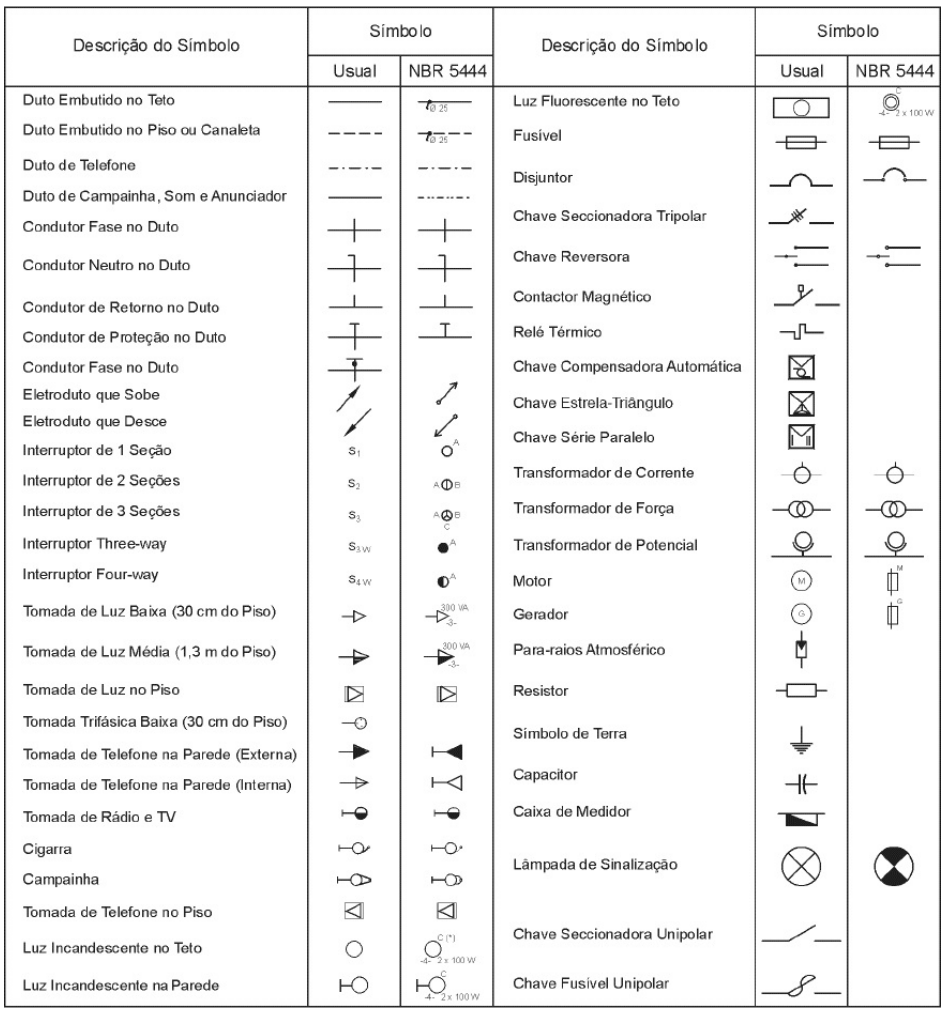
\includegraphics[width=\textwidth]{Figures/5. Symbology/NBR 5444.png}
		\caption{Algumas das simbologias gráficas para projetos da NBR 5444 - referência \cite{filho2017instalacoes}}
		\label{fig: simbologia nbr5444}
	\end{figure}
\newpage

% Adds an appendix entry
\section{Appendix B detalhes} \label{appendix: appendix B detalhes}

\tikz[remember picture,overlay]\node[anchor=south,inner sep=0pt] at (current page.south) {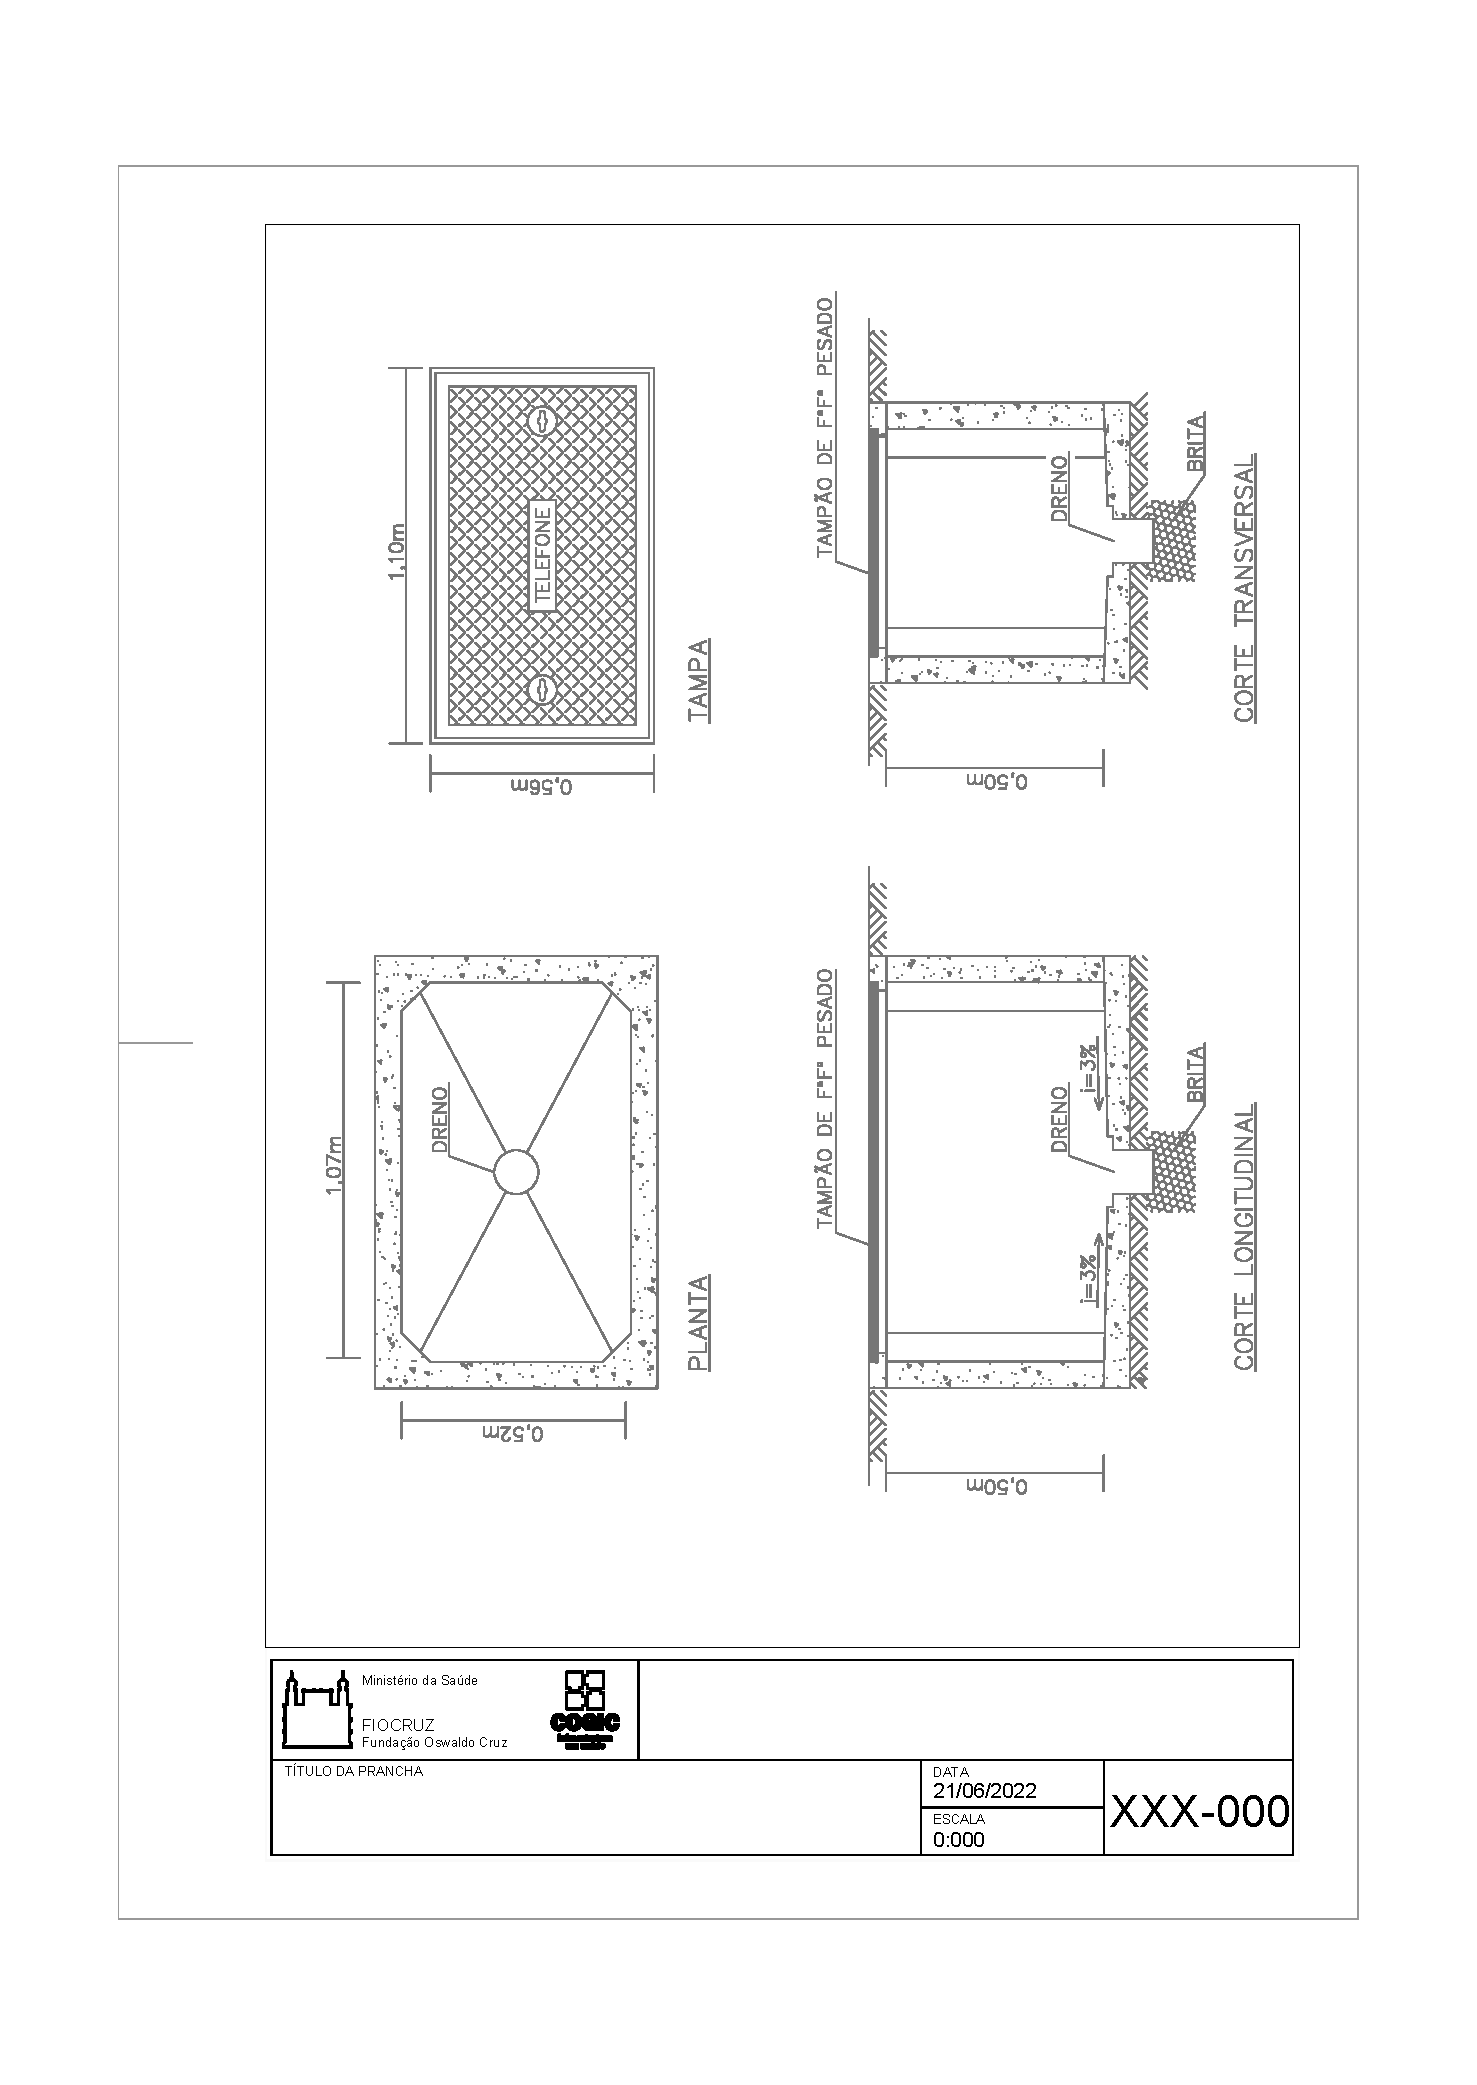
\includegraphics[width=\paperwidth]{Appendix/DET-1.pdf}};

\mbox{}
\vfill
\sffamily \Large \textcolor{white}{\placeanddate}

\newpage

\tikz[remember picture,overlay]\node[anchor=south,inner sep=0pt] at (current page.south) {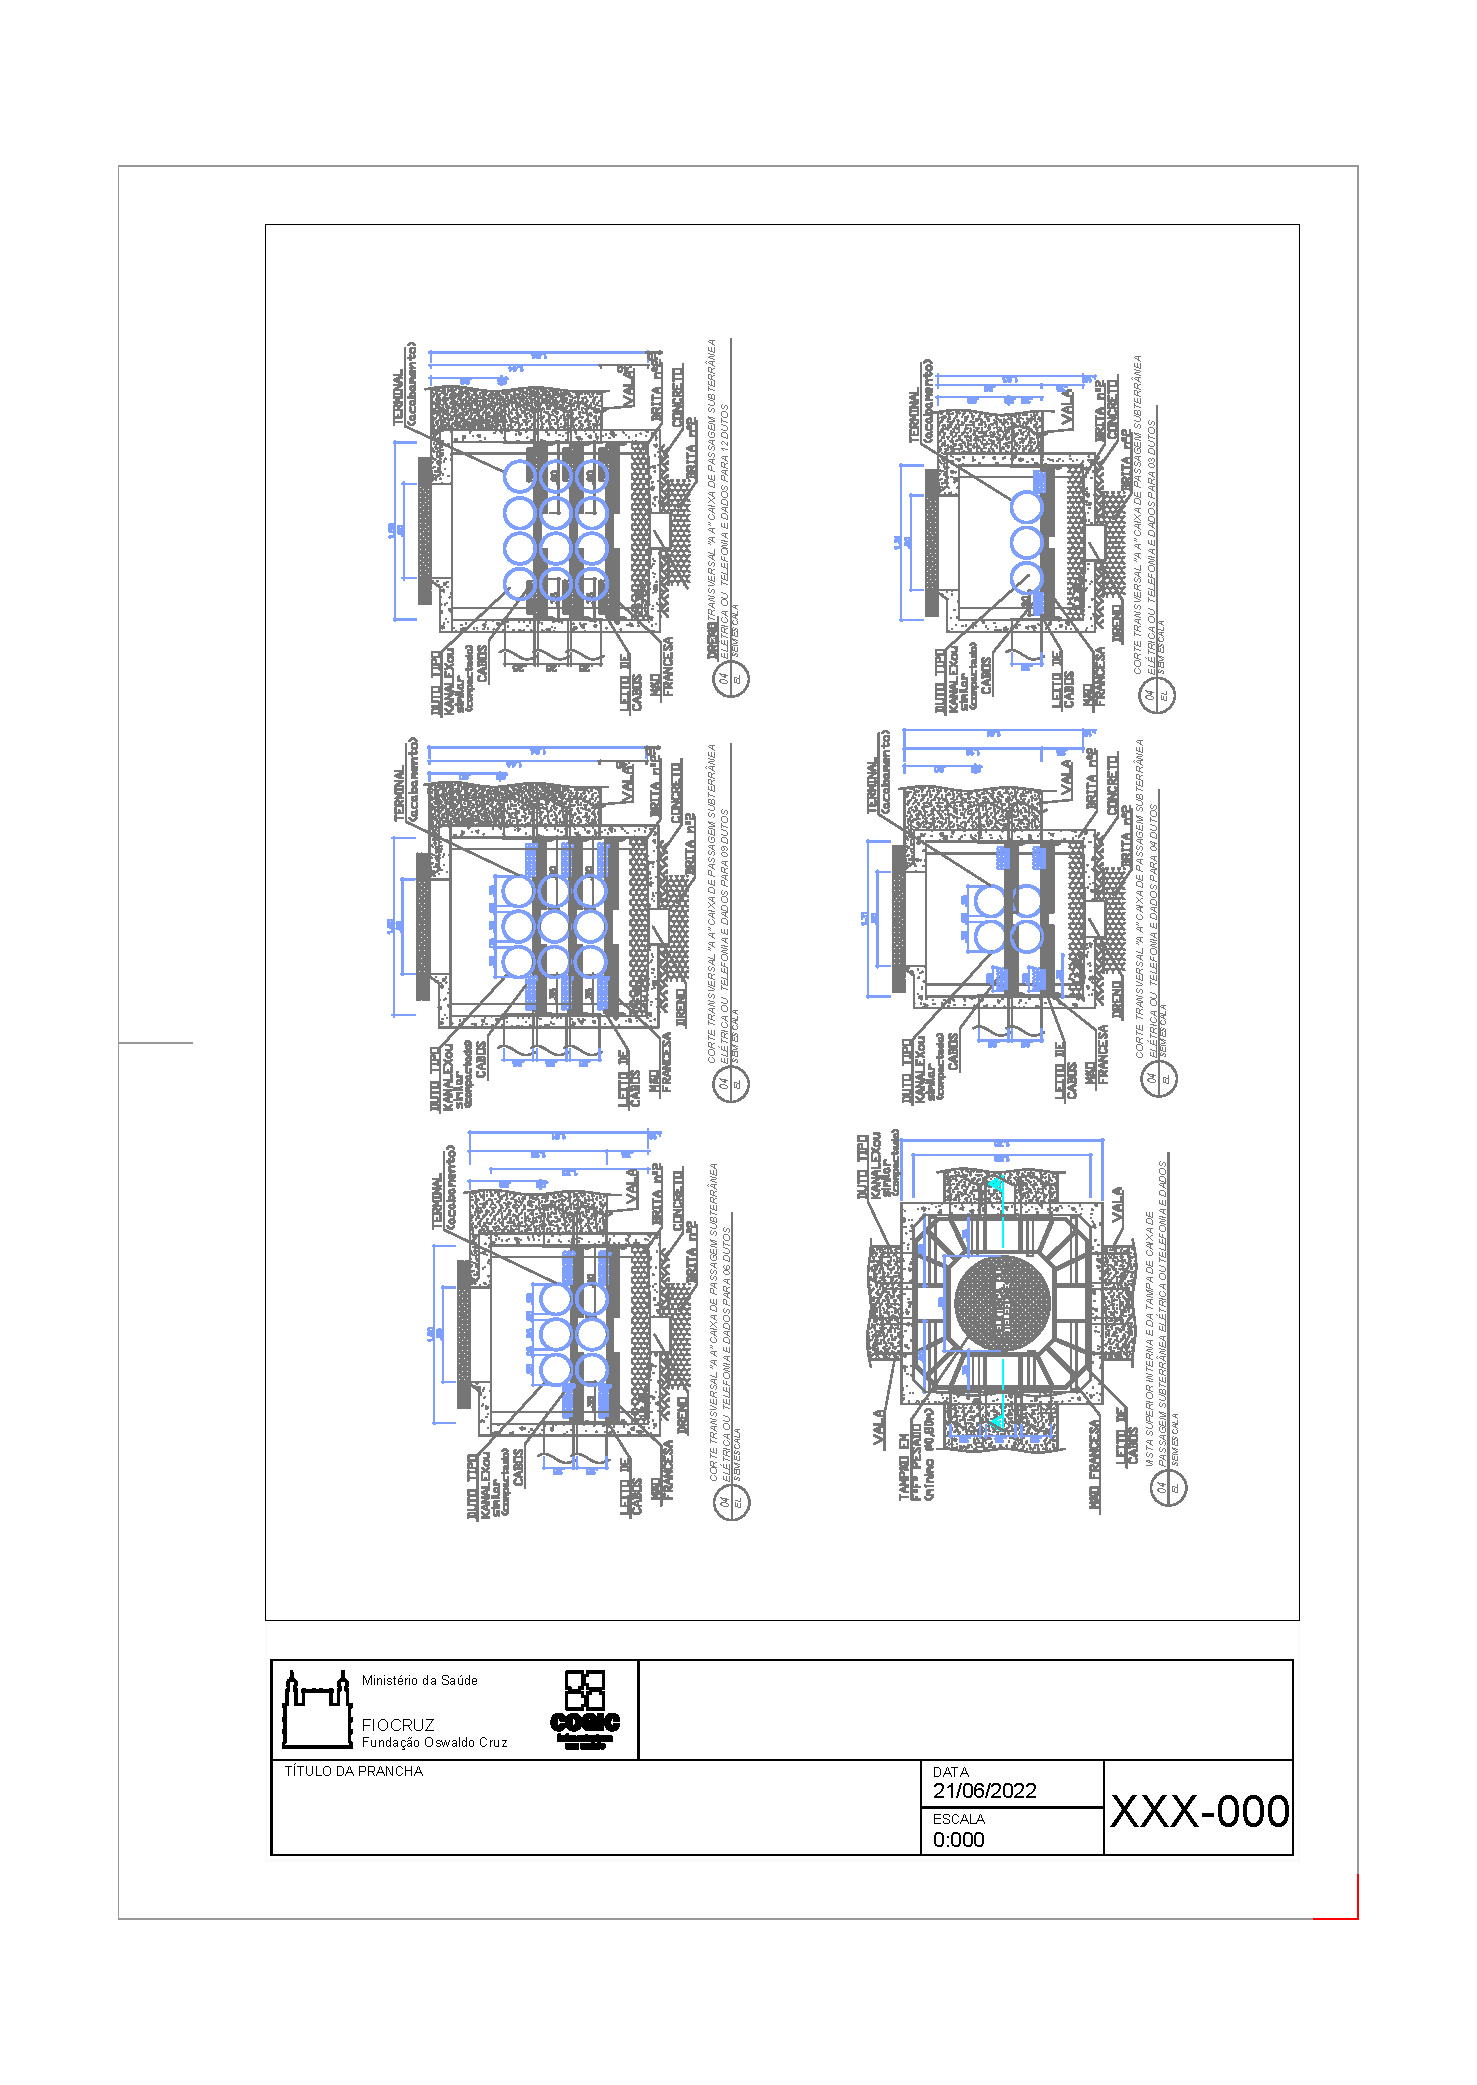
\includegraphics[width=\paperwidth]{Appendix/DET-2.pdf}};

\mbox{}
\vfill
\sffamily \Large \textcolor{white}{\placeanddate}

\newpage

\tikz[remember picture,overlay]\node[anchor=south,inner sep=0pt] at (current page.south) {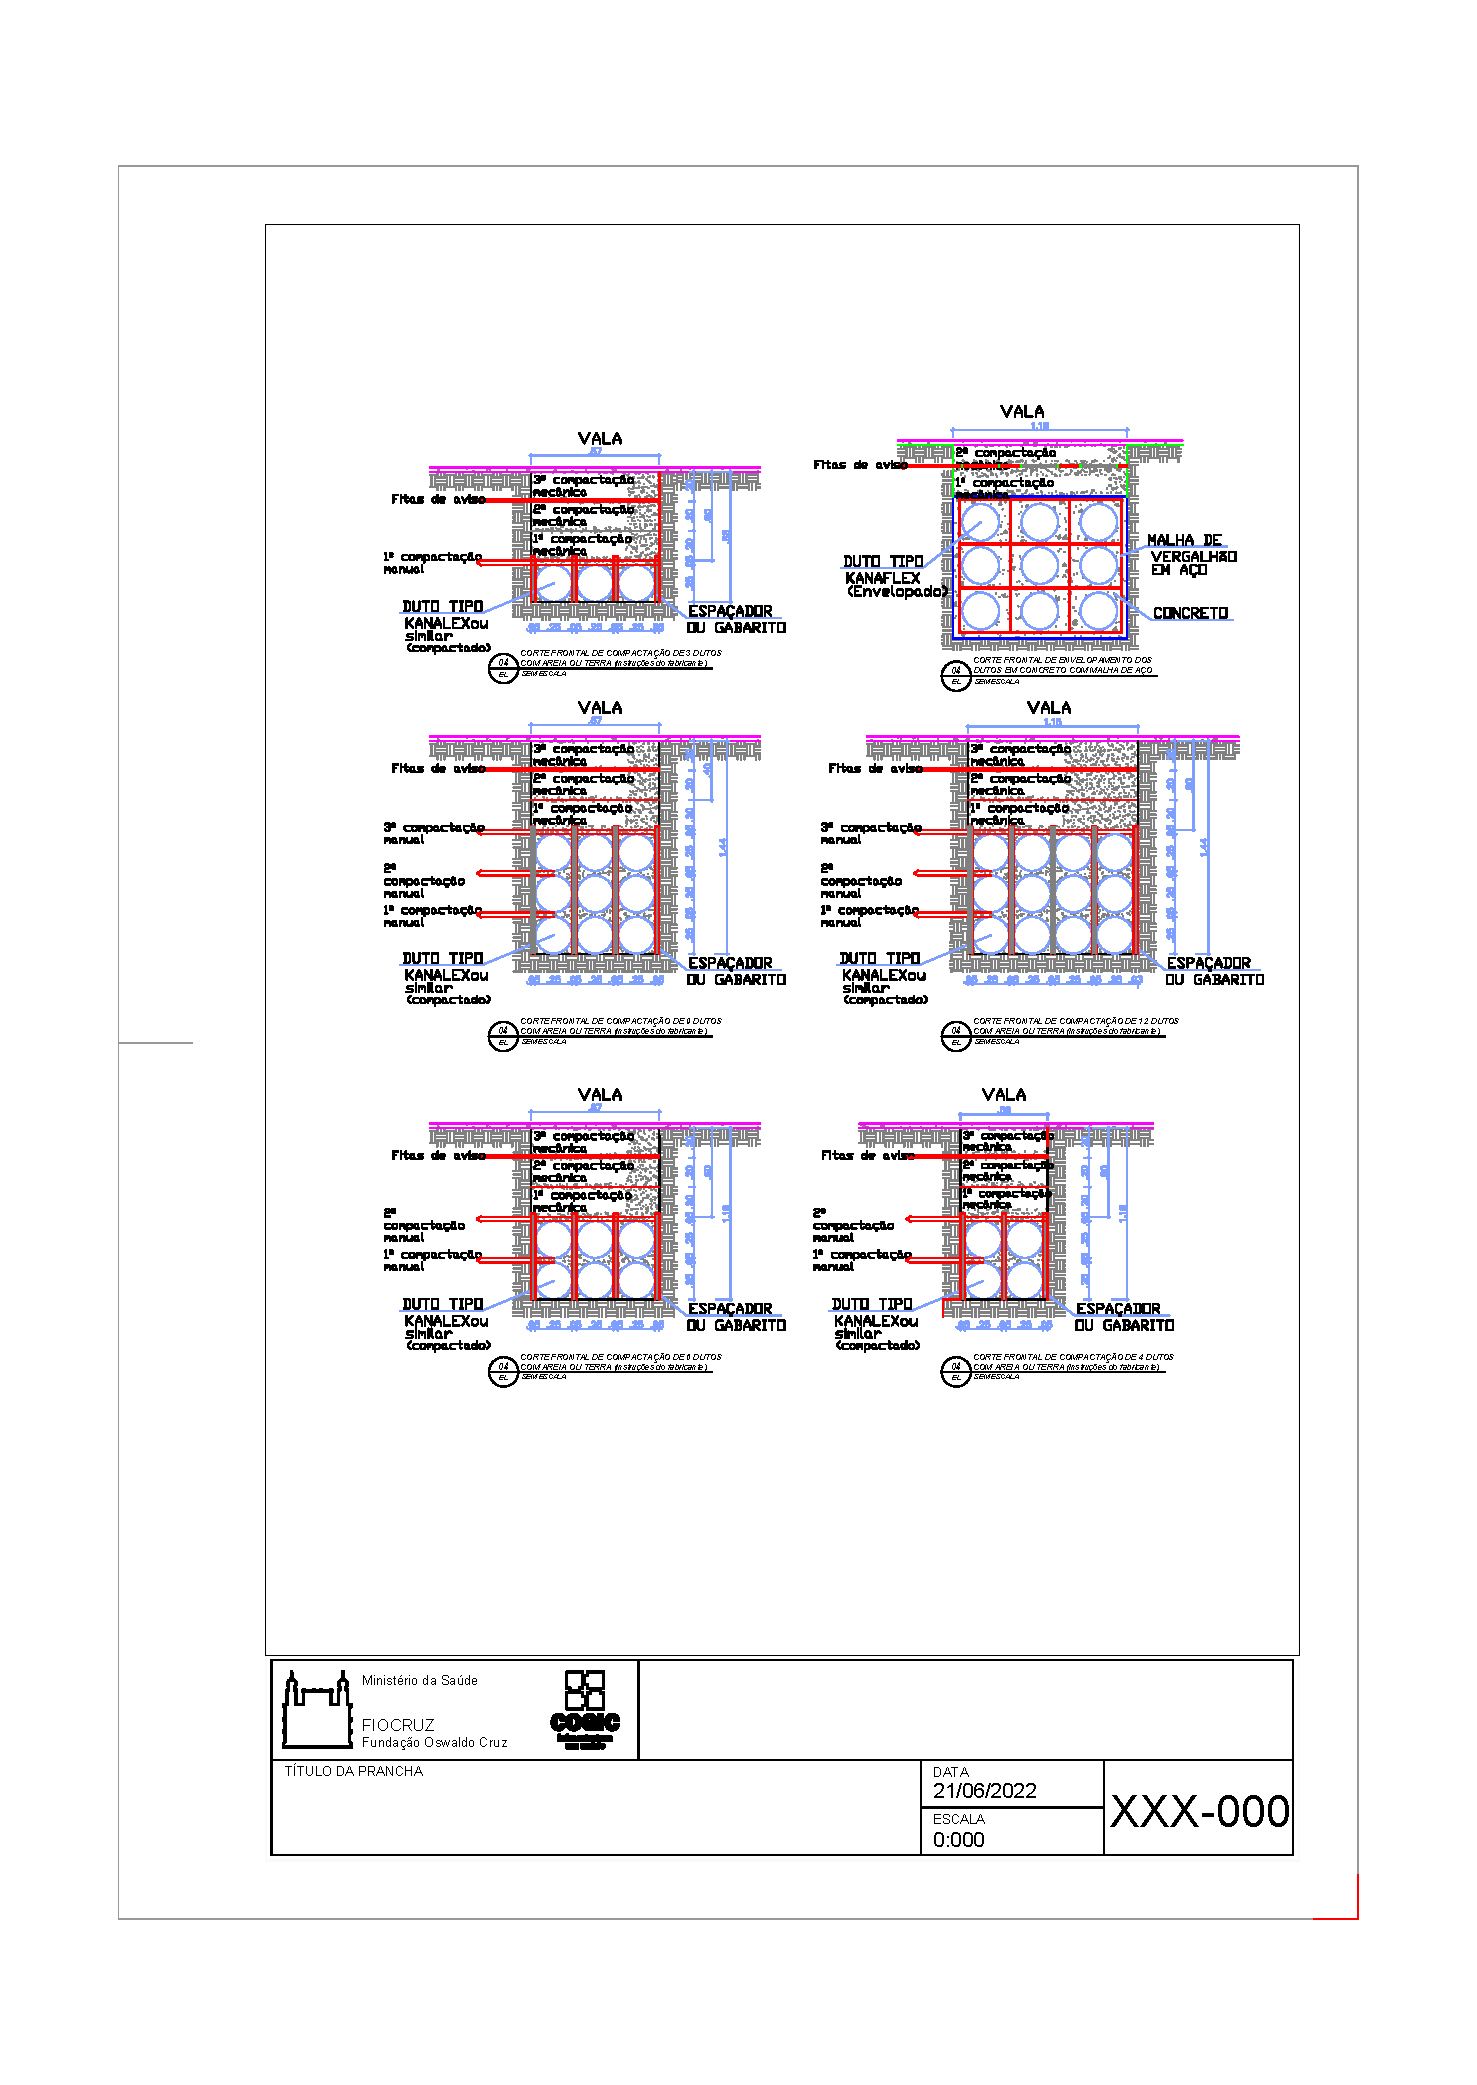
\includegraphics[width=\paperwidth]{Appendix/DET-3.pdf}};

\mbox{}
\vfill
\sffamily \Large \textcolor{white}{\placeanddate}

\newpage

\tikz[remember picture,overlay]\node[anchor=south,inner sep=0pt] at (current page.south) {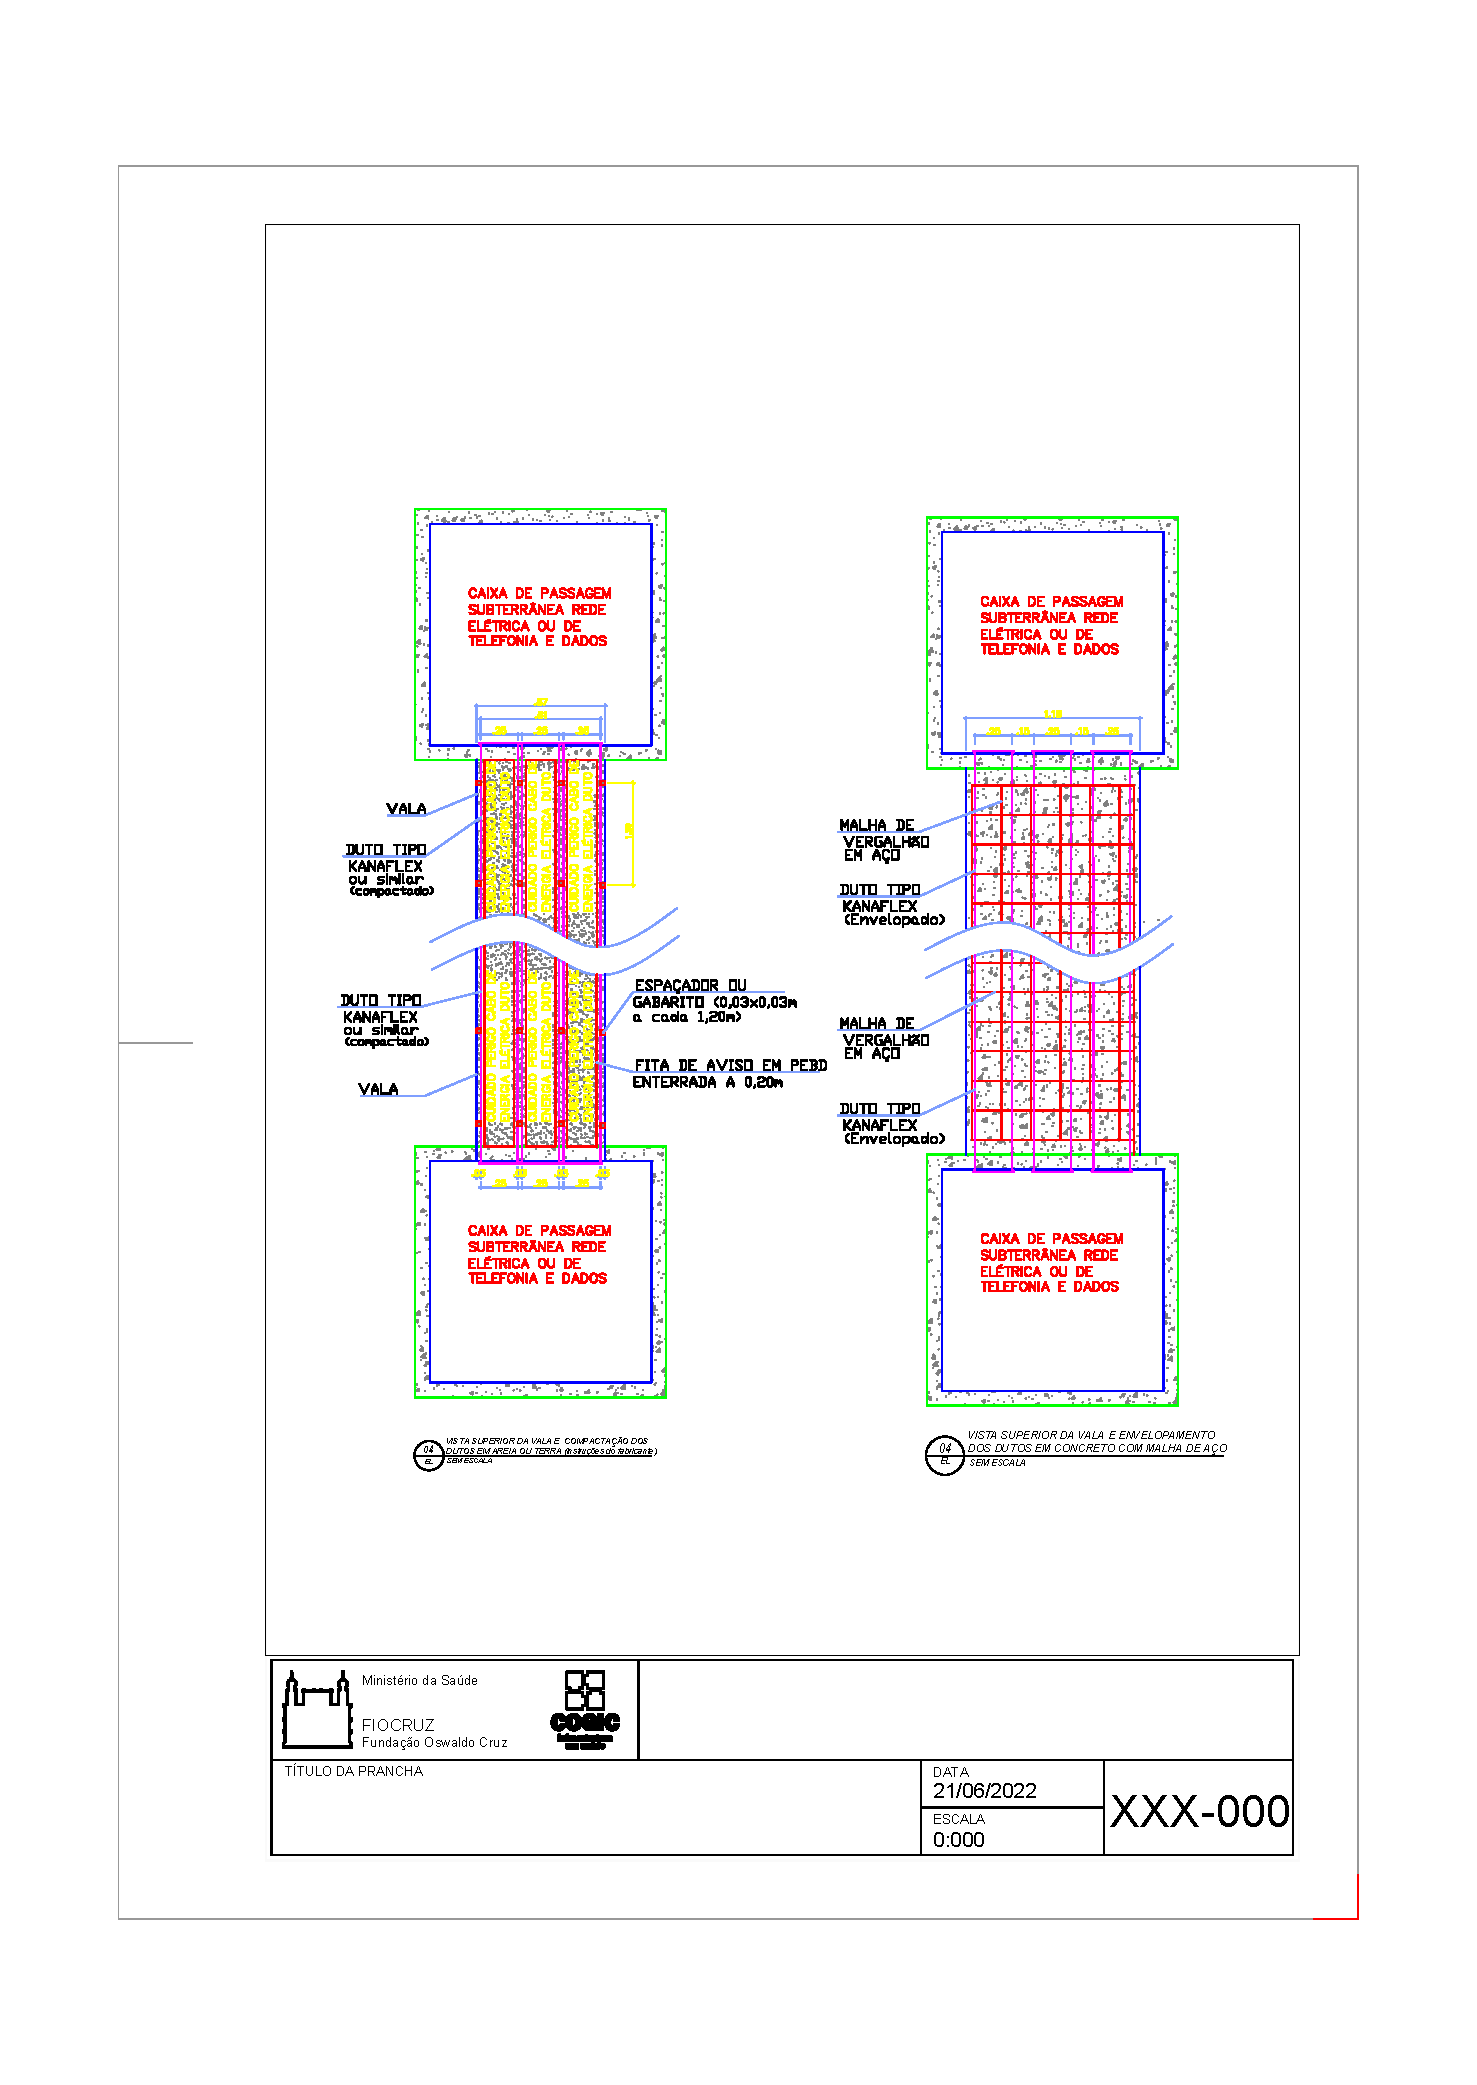
\includegraphics[width=\paperwidth]{Appendix/DET-4.pdf}};

\mbox{}
\vfill
\sffamily \Large \textcolor{white}{\placeanddate}

\newpage

\tikz[remember picture,overlay]\node[anchor=south,inner sep=0pt] at (current page.south) {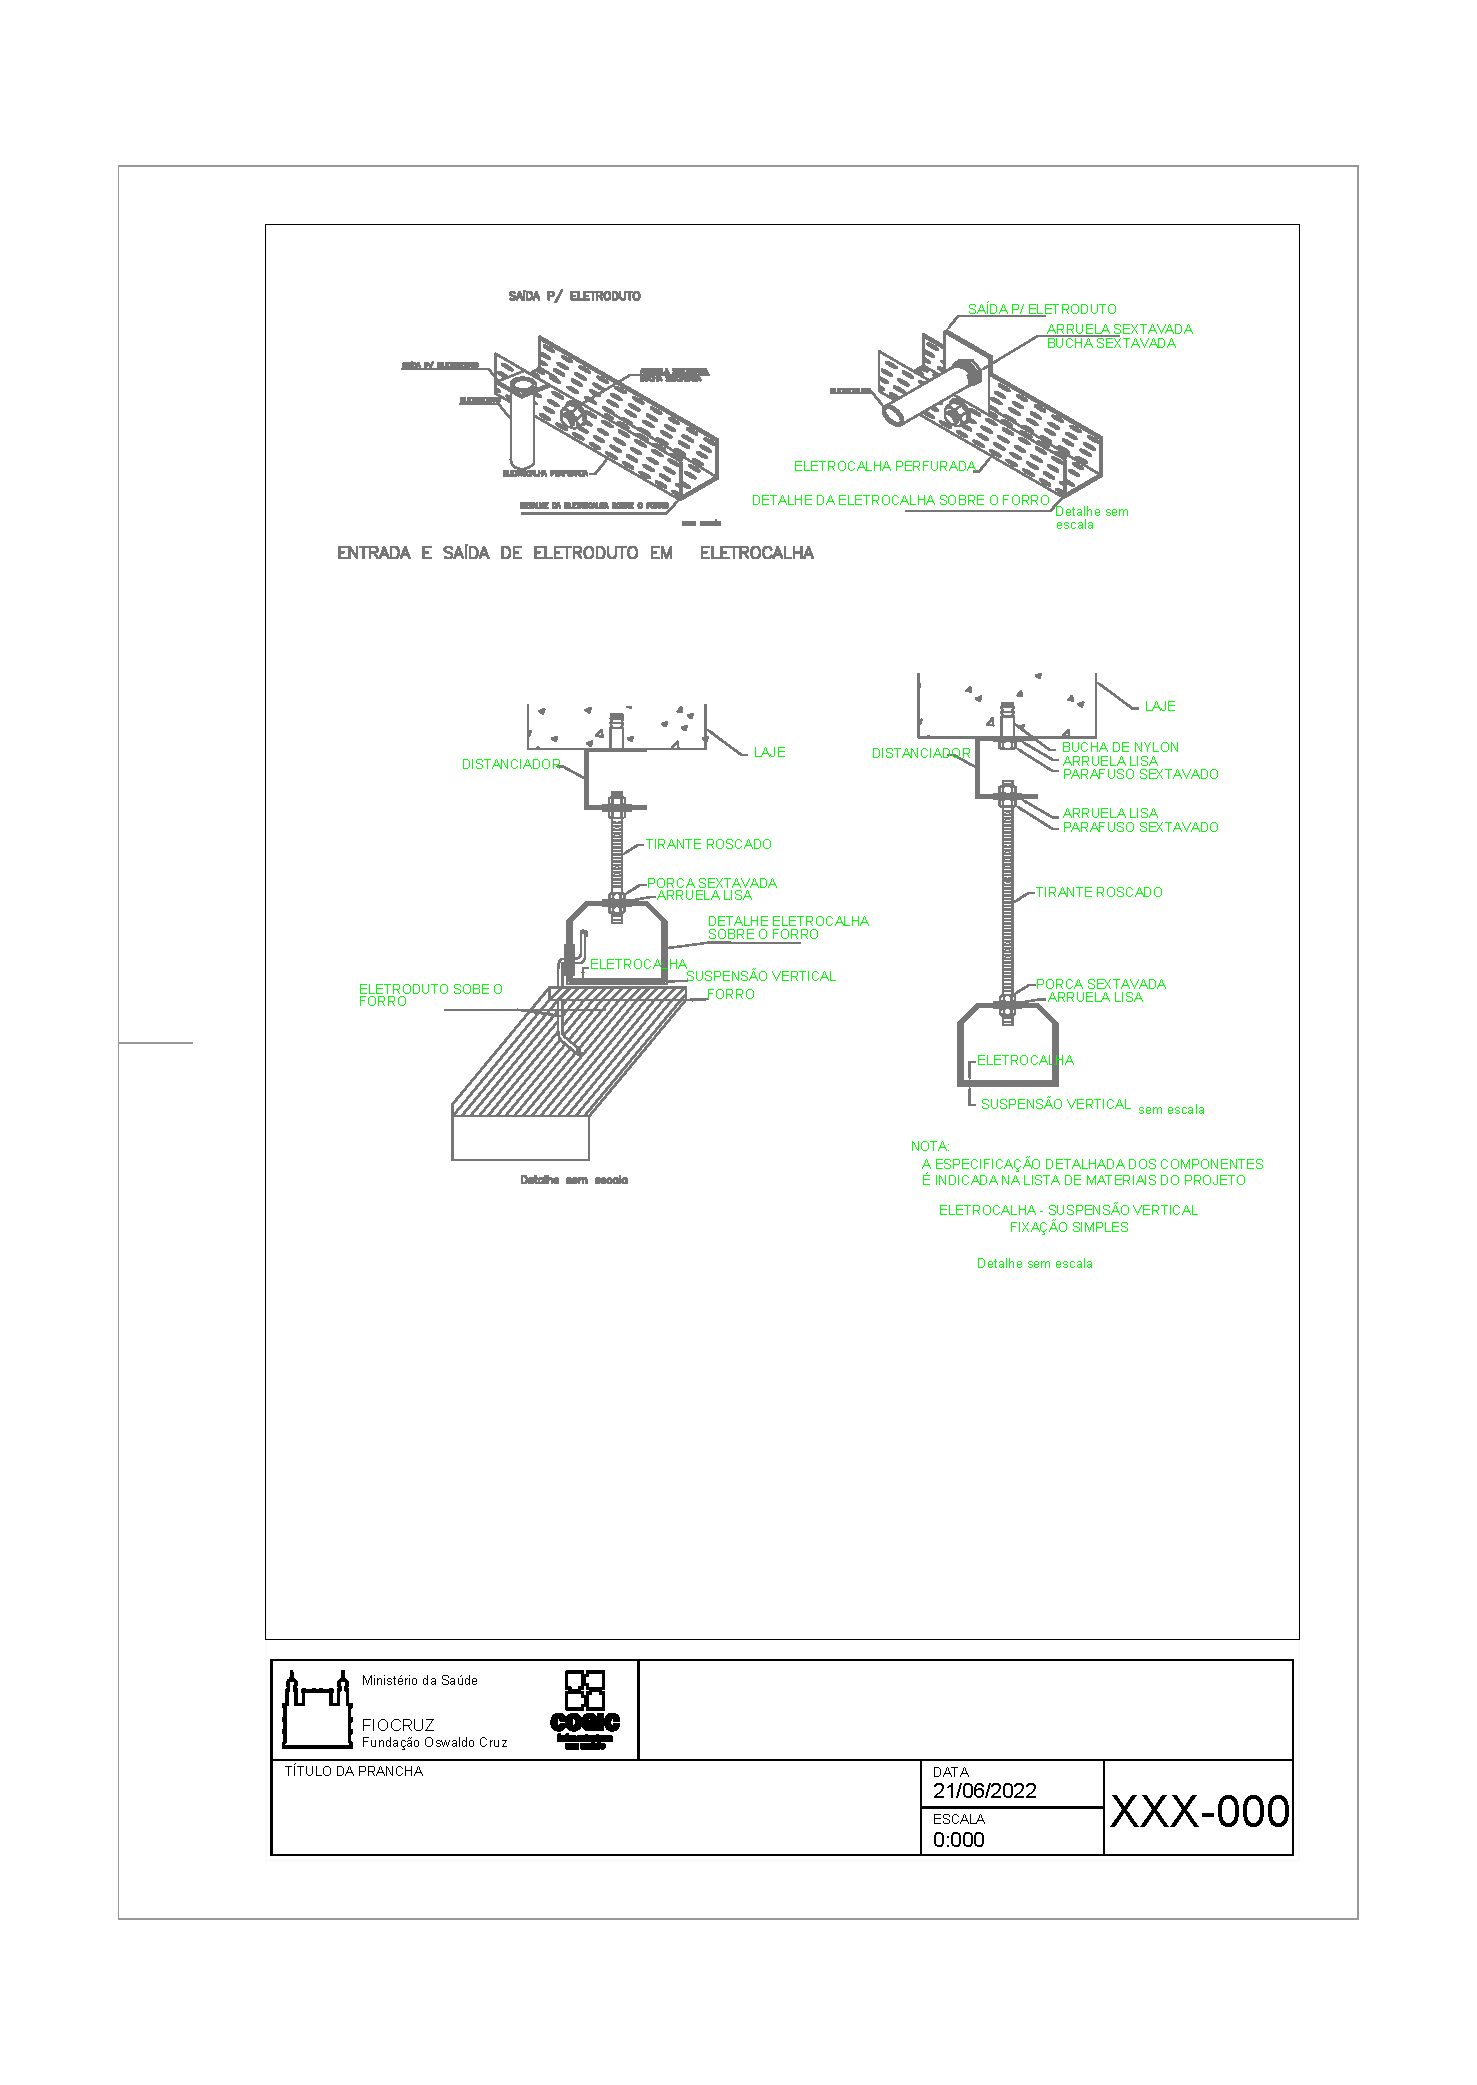
\includegraphics[width=\paperwidth]{Appendix/DET-5.pdf}};
\mbox{}
\vfill
\sffamily \Large \textcolor{white}{\placeanddate}

\newpage

\tikz[remember picture,overlay]\node[anchor=south,inner sep=0pt] at (current page.south) {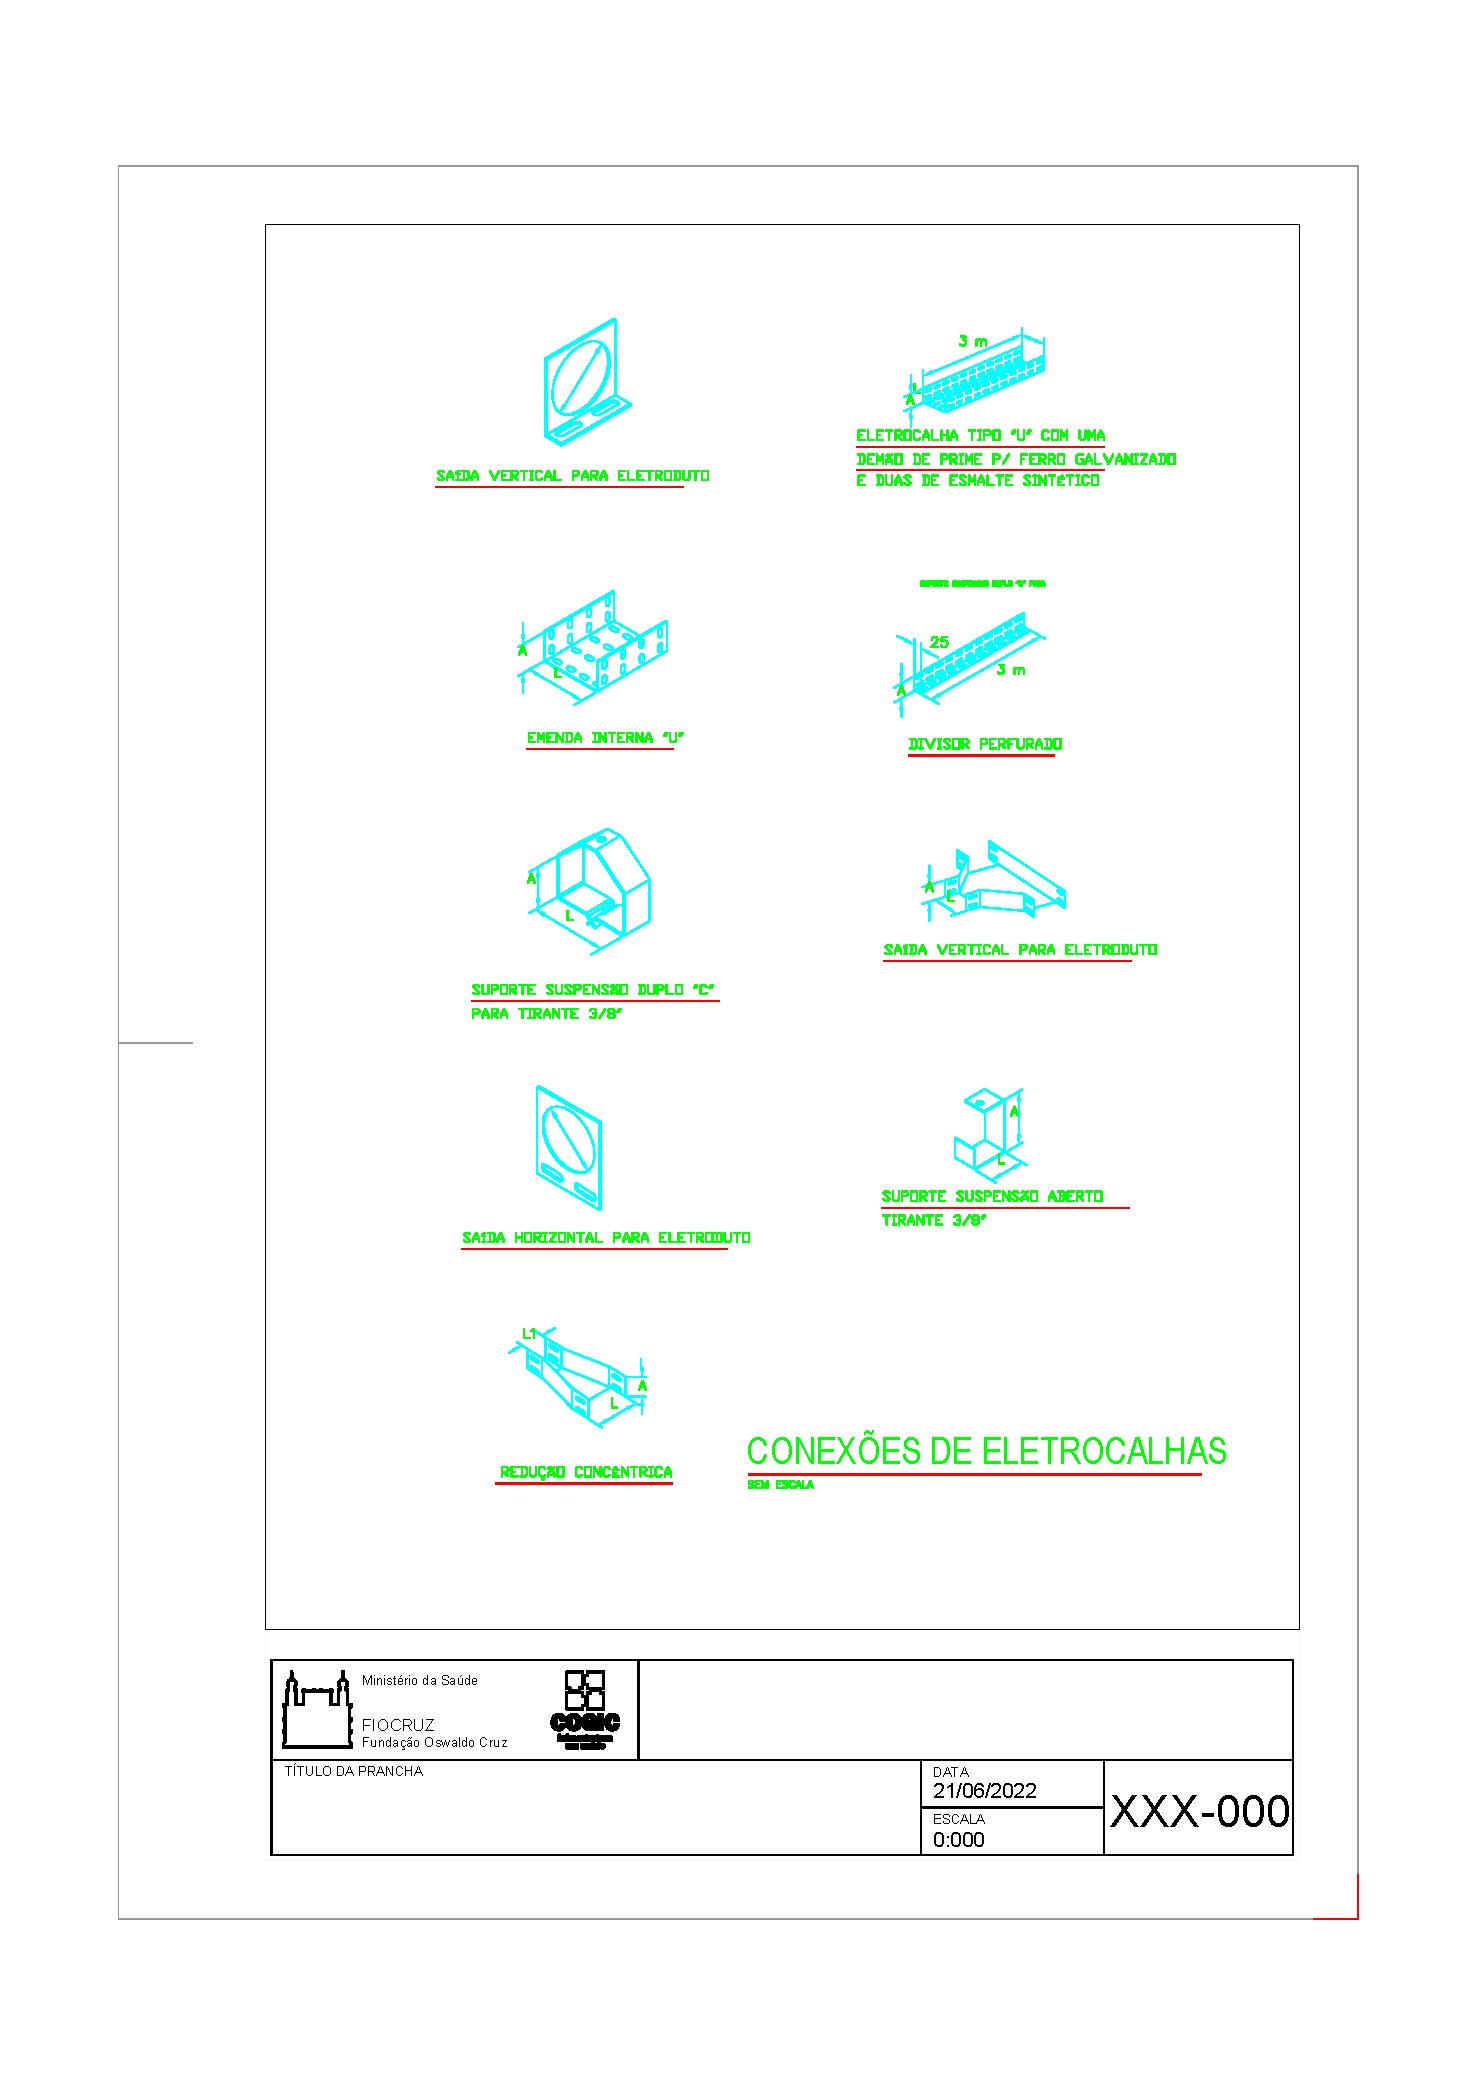
\includegraphics[width=\paperwidth]{Appendix/DET-6.pdf}};

\mbox{}
\vfill
\sffamily \Large \textcolor{white}{\placeanddate}

\newpage

\newpage

\end{document}
